\documentclass[12pt,a4paper]{report}
\usepackage[top=2.5cm, bottom=2.5cm, left=2.5cm, right=2.5cm]{geometry}

% Différentes options pour la classe :
% - taille de la fonte    : 10pt, 11pt, 12pt
% - recto ou recto-verso    : oneside, twoside
% - stade de développement    : draft, final


\usepackage[francais]{babel}
\usepackage[utf8]{inputenc} 
\usepackage[latin1]{inputenc}    % Pour utiliser les lettres accentuées
\usepackage{babel,blindtext}
\usepackage{float}
\usepackage[T1]{fontenc}
%\usepackage[francais,english]{babel}%          gestion du français
\usepackage{textcomp}%                 caractères additionnels
\usepackage{multirow}
\usepackage{supertabular}
\usepackage[pdftex]{graphicx}
\usepackage{setspace}
\usepackage{hyperref}
\usepackage[french]{varioref}
\usepackage{fancyhdr}
\usepackage{color}
\usepackage{colortbl}
\usepackage{amsmath}
\usepackage{ifpdf} % part of the hyperref bundle
\usepackage{array}
\usepackage{wrapfig}
\usepackage[table,xcdraw]{xcolor}

%\usepackage{abstract}


 % set fonts for nicer pdf view
 \IfFileExists{lmodern.sty}{\usepackage{lmodern}}{}


\pagestyle{fancy}
\fancyhead[L]{\nouppercase\leftmark} %pour afficher le nom du chapitre à gauche
\fancyhead[C]{}
\fancyhead[R]{\nouppercase\rightmark} %pour afficher le nom de la section à droite


\fancyfoot[L]{}
\fancyfoot[C]{}
\fancyfoot[R]{\textbf{\thepage}}

% Début du document
\begin{document}

%%%%%%%%%%%%%%%%%%%%%%%%%%%%%%%%%%%%%%%%%
% University Assignment Title Page 
% LaTeX Template
% Version 1.0 (27/12/12)
%
% This template has been downloaded from:
% http://www.LaTeXTemplates.com
%
% Original author:
% WikiBooks (http://en.wikibooks.org/wiki/LaTeX/Title_Creation)
%
% License:
% CC BY-NC-SA 3.0 (http://creativecommons.org/licenses/by-nc-sa/3.0/)
% 
% Instructions for using this template:
% This title page is capable of being compiled as is. This is not useful for 
% including it in another document. To do this, you have two options: 
%
% 1) Copy/paste everything between \begin{document} and \end{document} 
% starting at \begin{titlepage} and paste this into another LaTeX file where you 
% want your title page.
% OR
% 2) Remove everything outside the \begin{titlepage} and \end{titlepage} and 
% move this file to the same directory as the LaTeX file you wish to add it to. 
% Then add \input{./title_page_1.tex} to your LaTeX file where you want your
% title page.
%
%%%%%%%%%%%%%%%%%%%%%%%%%%%%%%%%%%%%%%%%%



\begin{titlepage}

\newcommand{\HRule}{\rule{\linewidth}{0.5mm}} % Defines a new command for the horizontal lines, change thickness here

\center % Center everything on the page
 
%----------------------------------------------------------------------------------------
%	HEADING SECTIONS
%----------------------------------------------------------------------------------------


\begin{minipage}[l]{0.2\columnwidth}

\includegraphics[width=3cm,height=2cm]{logo_istic.jpg}\\
\end{minipage}
\hfill
\begin{minipage}[l]{0.5\columnwidth}
\centering
\footnotesize
\textbf{\textsc{République Tunisienne}}\\
\textbf{\textsc{Ministère de l'Enseignement Supérieur\\
et de la Recherche Scientifique}}\\
\medskip 
\textbf{\textsc{Université de Carthage}}\\
\medskip 
\textbf{\textsc{Institut Supérieur des Technologies de l'Information et de la Communication}}
\end{minipage}
\hfill
\begin{minipage}[l]{0.2\columnwidth}

\includegraphics[width=3cm,height=3cm]{universite-carthage.jpg}\\
\end{minipage}

\vskip1cm
\textsc{\large Rapport de Projet de Fin d'Etudes}\\[0.5cm] % Minor heading such as course title\\

\textbf{Présenté en vue de l'obtention de la}

\textsc{\large Licence Fondamentale en Sciences et Technologies}\\[0.5cm] % Minor heading such as course title\\

\textbf{Mention: Sciences de l'Informatique}

\textbf{Spécialité : Sciences de l'Informatique}

\vskip1cm%

%----------------------------------------------------------------------------------------
%	TITLE SECTION
%----------------------------------------------------------------------------------------

\HRule \\[0.4cm]
\textcolor{blue}{ \LARGE \bfseries Intitulé du projet}\\[0.4cm] % Title of your document
\HRule \\[1cm]

\vskip0.5cm%
\textit{Par}\\
\textsc{\large Prénom NOM}\\[0.5cm] % Minor heading
\vskip0.5cm%

%\vspace{0.5cm}
%\begin{center}
{Réalisé au sein de Tunisie Télécom}\\
%\smallskip

\includegraphics[width=0.2\columnwidth]{tt-logo.jpg}\\
%\end{center}

\vskip1cm
 
%----------------------------------------------------------------------------------------
%	Supervisor SECTION
%----------------------------------------------------------------------------------------
 \begin{flushleft}
Soutenu publiquement le ? mai 2019 devant le jury composé de :
\smallskip

\begin{minipage}[c]{0.3\columnwidth}
Président:\\
Rapporteur:\\
Examinateur:\\
Encadrant professionnel:\\
Encadrant académique:
\end{minipage}
%\hfill
\begin{minipage}[c]{0.6\columnwidth}
Prénom NOM, University Relations Leader, IBM\\
Prénom NOM, Enseignant, ISTIC\\
Prénom NOM, Enseignant, ISTIC\\
Prénom NOM, Ingénieur, VERMEG\\
Prénom NOM, Enseignant, ISTIC
\end{minipage}
%\begin{minipage}[c]{0.4\columnwidth}
%{\small Maitre-Assistant en Informatique}\\
%{\small Maitre-Assistant en Informatique}\\
%{\small Maitre-Assistant en Télécommunications}\\
%{\small Ingénieur}\\
%{\small Assistant en Informatique}
%\end{minipage}
 \end{flushleft}

%----------------------------------------------------------------------------------------
%	DATE SECTION
%----------------------------------------------------------------------------------------
\vskip2cm

{\large Année Universitaire: 2018-2019}\\[3cm] 



\vfill % Fill the rest of the page with whitespace

\end{titlepage}
%\end{document}
%%%%%%%%%%%%%%%%%%%%%%%%%%%%%%%%%%%%%%%%%
% University Assignment Title Page 
% LaTeX Template
% Version 1.0 (27/12/12)
%
% This template has been downloaded from:
% http://www.LaTeXTemplates.com
%
% Original author:
% WikiBooks (http://en.wikibooks.org/wiki/LaTeX/Title_Creation)
%
% License:
% CC BY-NC-SA 3.0 (http://creativecommons.org/licenses/by-nc-sa/3.0/)
% 
% Instructions for using this template:
% This title page is capable of being compiled as is. This is not useful for 
% including it in another document. To do this, you have two options: 
%
% 1) Copy/paste everything between \begin{document} and \end{document} 
% starting at \begin{titlepage} and paste this into another LaTeX file where you 
% want your title page.
% OR
% 2) Remove everything outside the \begin{titlepage} and \end{titlepage} and 
% move this file to the same directory as the LaTeX file you wish to add it to. 
% Then add \input{./title_page_1.tex} to your LaTeX file where you want your
% title page.
%
%%%%%%%%%%%%%%%%%%%%%%%%%%%%%%%%%%%%%%%%%



\begin{titlepage}

\newcommand{\HRule}{\rule{\linewidth}{0.5mm}} % Defines a new command for the horizontal lines, change thickness here

\center % Center everything on the page
 
%----------------------------------------------------------------------------------------
%	HEADING SECTIONS
%----------------------------------------------------------------------------------------


\begin{minipage}[l]{0.2\columnwidth}

\includegraphics[width=3cm,height=2cm]{logo_istic.jpg}\\
\end{minipage}
\hfill
\begin{minipage}[l]{0.5\columnwidth}
\centering
\footnotesize
\textbf{\textsc{République Tunisienne}}\\
\textbf{\textsc{Ministère de l'Enseignement Supérieur\\
et de la Recherche Scientifique}}\\
\medskip 
\textbf{\textsc{Université de Carthage}}\\
\medskip 
\textbf{\textsc{Institut Supérieur des Technologies de l'Information et de la Communication}}
\end{minipage}
\hfill
\begin{minipage}[l]{0.2\columnwidth}

\includegraphics[width=3cm,height=3cm]{universite-carthage.jpg}\\
\end{minipage}

\vskip1cm
\textsc{\large Rapport de Projet de Fin d'Etudes}\\[0.5cm] % Minor heading such as course title\\

\textbf{Présenté en vue de l'obtention de la}

\textsc{\large Licence Fondamentale en Sciences et Technologies}\\[0.5cm] % Minor heading such as course title\\

\textbf{Mention: Sciences de l'Informatique}

\textbf{Spécialité : Sciences de l'Informatique}

\vskip1cm%

%----------------------------------------------------------------------------------------
%	TITLE SECTION
%----------------------------------------------------------------------------------------

\HRule \\[0.4cm]
\textcolor{blue}{ \LARGE \bfseries Intitulé du projet}\\[0.4cm] % Title of your document
\HRule \\[1cm]

\vskip0.5cm%
\textit{Par}\\
\textsc{\large Prénom NOM}\\[0.5cm] % Minor heading
\vskip0.5cm%

%\vskip1cm%
%\begin{center}
{Réalisé au sein de Tunisie Télécom}\\
%\smallskip

\includegraphics[width=0.2\columnwidth]{tt-logo.jpg}\\
%\end{center}

\vskip1cm
 
%----------------------------------------------------------------------------------------
%	Supervisor SECTION
%----------------------------------------------------------------------------------------


 \begin{flushleft}
\textbf{\textsc{Autorisation de dépôt du rapport de Projet de Fin d'Etudes:}}\\[0.5cm] % Minor heading
\vskip0.5cm
\begin{minipage}[c]{0.3\columnwidth}
Encadrant professionnel:\\
\vskip0.5cm
Le:\\
\vskip0.5cm
Signature:\\

\end{minipage}
\hfill
\begin{minipage}[c]{0.4\columnwidth}
Encadrant académique:\\
\vskip0.5cm
Le:\\
\vskip0.5cm
Signature:\\
\end{minipage}

 \end{flushleft}

%----------------------------------------------------------------------------------------
%	DATE SECTION
%----------------------------------------------------------------------------------------
%\vskip1cm
%{\large Année Universitaire: 2016-2017}\\[3cm] 



\vfill % Fill the rest of the page with whitespace

\end{titlepage}
%\end{document}
\newpage
\pagenumbering{roman}
\chapter*{Dédicaces}
\addcontentsline{toc}{chapter}{Dédicaces}

\noindent A mes parents,
\\
A mes frères et s\oe urs,
\\
A mes amis 


\chapter*{Remerciements}
\addcontentsline{toc}{chapter}{Remerciements}

Je tiens à remercier 


\tableofcontents    % Table des matières
\listoffigures        % Liste des figures
\listoftables        % Liste des tableaux
\newpage
\pagenumbering{arabic}

\chapter*{Introduction Générale}
\markboth{Introduction Générale}{} %pour afficher l'entete
\addcontentsline{toc}{chapter}{Introduction Générale}
Les solutions technologiques autour des infrastructures distribuées n'arrêtent pas de progresser, les sociétés consommatrices deviennent de plus en plus nombreux, ils sont aujourd'hui au centre
de tous ces changements.\\\\ Actuellement, une nouvelle tendance a fait son apparition dans le monde des technologies
de l'information. Il s'agit du «Cloud computing». Ce
modèle a récemment émergé comme un nouveau paradigme pour l'hébergement
et la prestation de services sur Internet. Le Cloud computing est le nouveau pas
dans l'évolution des services web et des produits informatiques à la demande.\\\\
A ce niveau, le Cloud computing se déplace comme un remède offrant une architecture distante dont la gestion est garantie par une tierce partie. Le fournisseur de cette architecture garantit par conséquent l'utilisation et le suivi des services à travers des plateformes tel que Google Cloud Plateform  pour le fournisseur Google.\\\\ Bien que  le genre de ces plateformes semble idéal pour la gestion des ressources Cloud. Cependant, ils ne peuvent pas être personnalisées au besoin de l'entreprise. C'est ainsi qu'une mauvaise utilisation des ressources  augmente les dépenses de l'entreprise. Le contrôle des ressources devient  alors impensable pour les entreprises consommatrices du Cloud.\\\\
C'est dans ce cadre que l'équipe Tritux a eu l'idée de créer une
application permettant de gèrer leurs ressources Cloud par projet et budget grâce aux nouvelles technologies de l'information.\\
Ce projet s'est déroulé selon l'esprit de la méthode agile du Scrum ainsi la répartition du rapport va simuler les différents sprints réalisés. Dans cette optique, nous introduisons le plan de ce rapport :\\\\
Nous introduisons dans le premier chapitre le contexte, les notions théoriques liées au projet et ses objectifs à
savoir les fonctionnalités envisagées, Nous présentons de même l'entreprise d'accueil,
ses domaines et la solution actuelle.\\
Le deuxième chapitre sera dédié à l'analyse et les spécifications fonctionnelles et non
fonctionnelles pour la réalisation de notre application.\\
Ensuite, nous entamerons la classification des chapitres selon la méthode Scrum c'est
à dire en sprint et chaque sprint abordera une ou plusieurs fonctionnalités de notre application de l'analyse jusqu'à la réalisation en passant par la conception.\\
Enfin nous terminerons par une conclusion qui établit le bilan du travail effectué et ouvre des
nouvelles perspectives pour améliorer l'application.


\chapter{Cadre général du projet}
    %\addcontentsline{toc}{chapter}{}

\section{Introduction}

Dans ce premier chapitre, nous présenterons le cadre général du projet. D'abord, nous
Commencerons  par  la présentation de  l'organisme  d'accueil.  Ensuite, nous  discuterons  la  problématique. Nous développerons
une étude de  l'existant.   Enfin,  nous  proposerons  une  solution  
à  cette  problématique  en  exposant  la  méthodologie  de  travail  que  nous  avons  suivi. 
\section{Présentation de l'organisme d'accueil }
Dans la partie qui suit, nous allons présenter l'organisme d'accueil, ses domaines, ses compétences ainsi que ses certifications.
\subsection{Présentation de l'organisme d'accueil}
TriTUX est une société internationale spécialisée dans l'ingénierie logicielle, le développement des systèmes d'informations, le conseil en informatique et l'externalisation.
Avec plus de 13 ans d'expérience, elle est l'un des principaux fournisseurs de solutions
informatiques et de télécommunication. Grâce à une infrastructure solide et à des multiples
certifications dans les nouvelles technologies, TriTUX fournit des services d'ingénierie et
de conseil en innovation et en agilité commerciale. Elle perçoit l'environnement commercial et la rentabilité de ses clients en proposant des solutions adaptées et personnalisées
avec un ensemble complet de services, de la conception à la mise en ?uvre.

\subsection{Solutions}
TriTUX est un partenaire stratégique dans :
\begin{itemize}
	\item \textbf{IoT}: Une large gamme de solutions IoT puissantes répondant aux besoins spécifiques des entreprises
\item \textbf{VAS}: Une large gamme de solutions à valeur ajoutée allant au-delà des normes
vocales, de messagerie et de télécopie.
\item \textbf{Roaming}: Des outils multifonctions gérant les défis opérationnels et commerciaux.
\item \textbf{Solutions informatiques}: Des solutions d'itinérance innovantes pour renforcer
l'image de marque de ses clients et maximiser leurs revenus.
\end{itemize}
\subsection{Domaines et compétences }
Tritux propose un large éventail de services de conseil, d'ingénierie et d'analyse.Ces
services s'adressent à la chaîne de valeur complète d'ingénierie couvrant divers secteurs :
\begin{itemize}
	\item Consulting et administration Unix et Base des données.
	\item Datawarehousing et business intelligence.
	\item Messagerie multimédia SMS/MMS/FAX/WAP/WEB.
	\item Conception de solutions critiques et à fortes charges.
	\item Systèmes d'information et services spécialisés dans l'architecture SOA.
\end{itemize}

\subsection{Collaborateurs}
TriTUX a su se hisser dans la cour des grands en se positionnant sur le marché et
en fidélisant de nombreux clients importants en Europe et en Afrique. Parmi celles-ci,
figurent notamment :
\begin{figure}[ht]
	\centering
	
\includegraphics[scale=0.5]{collaborateurs.png}
	\caption{Les collaborateurs de TRITUX}
	\label{Les collaborateurs de TRITUX}
\end{figure}

\subsection{Certifications}
TRITUX a déployé une infrastructure solide et des certifications reconnues dans le
domaine des nouvelles technologies répondant à toutes les exigences, en appliquant les
meilleures pratiques des secteurs public et privé du monde entier et en exploitant la technologie innovante.

Parmi les certificats acquis par TriTUX on note :
\begin{itemize}
	\item Certification en management de la qualité ISO 9001.
	\item International Software Testing Qualifications Board ISTQB.
	\item Oracle Java Certified Professional.
	\item Linux Red Hat certified engineer.
\end{itemize}
\subsection{Organigramme}
L'organisation hiérarchique de Tritux est présentée dans l'organigramme de la figure 1.2
suivante:
\begin{figure}[ht]
	\centering
	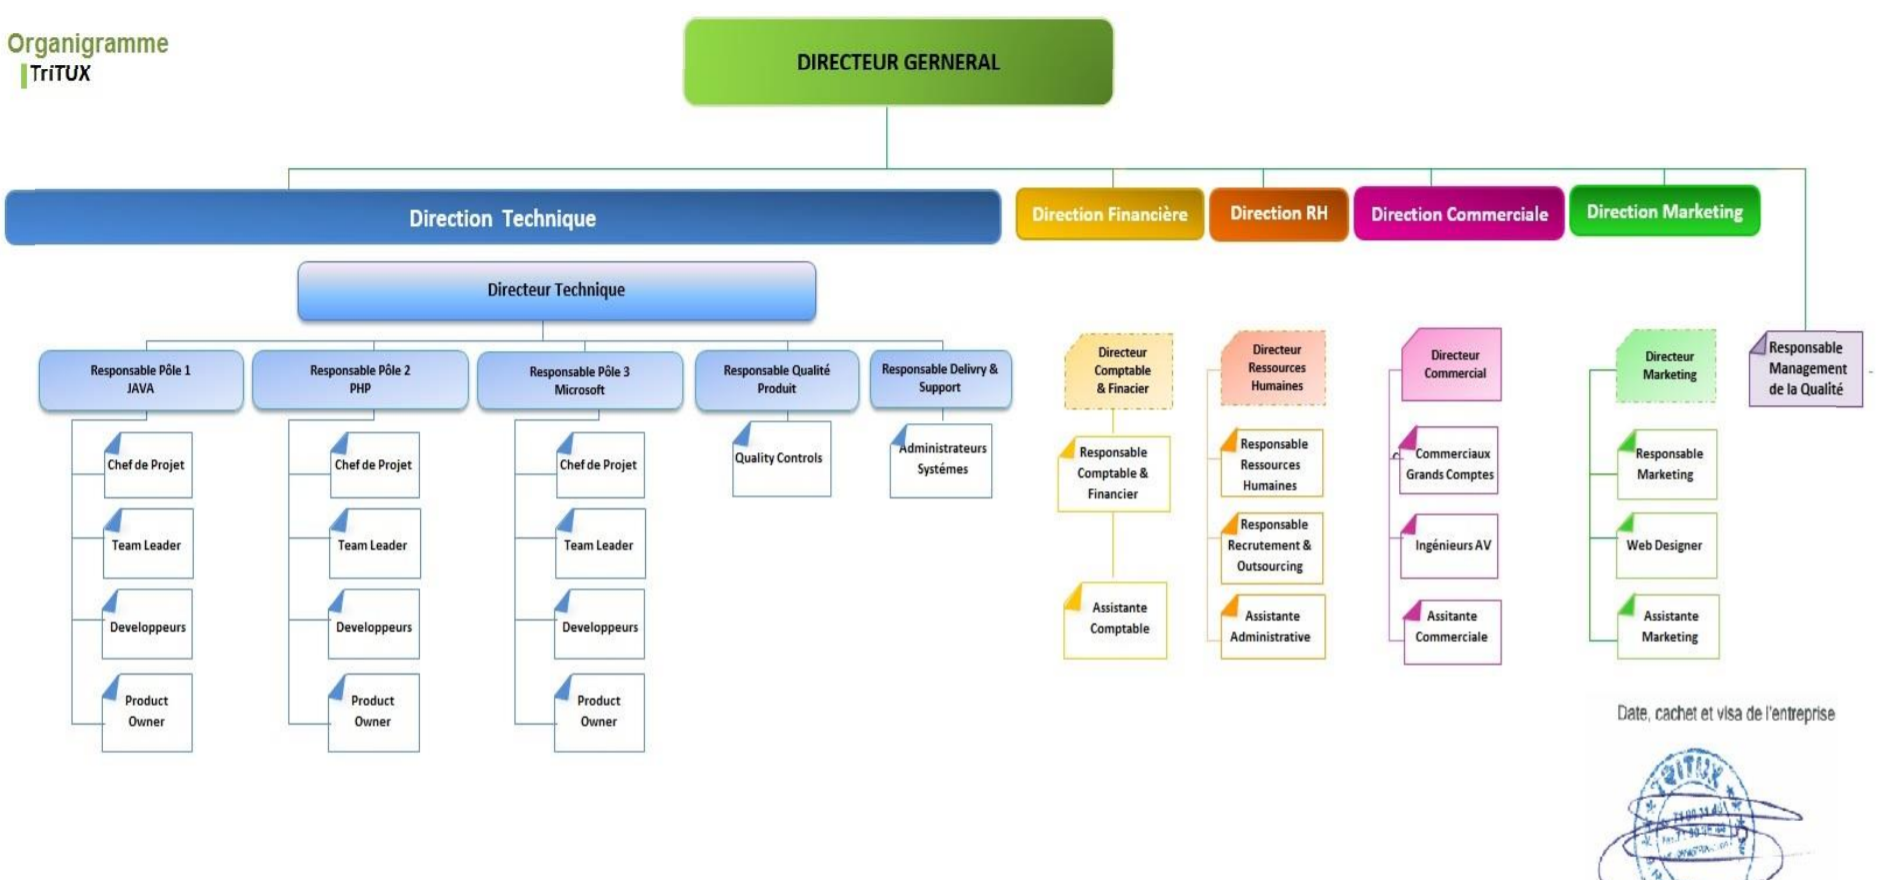
\includegraphics[width=18cm]{organigramme.PNG}
	\caption{Organigramme de TRITUX}
	\label{Organigramme de TRITUX}
\end{figure}
\newpage
\section {Cadre du projet}
\subsection{Contexte du projet}
Dans  le  cadre  de  l'optimisation  de  consommation  de  ses  ressources  et  la  diminution  de 
ses  dépenses,  Tritux  vise  à  mettre  en  place  une  plateforme  de  budgétisation  des  ressources 
Cloud.  Pour  ce  fait,  l'entreprise  d'accueil  nous  a  confié cette  tâche  de  conception  et 
développement  d'une  application  de  gestion  des  ressources  Cloud  par 
projet  et  budget. 



\subsection{Problématique}
Avant l'utilisation du Cloud les entreprises ont beaucoup souffert de la complexité de la gestion de leurs systèmes informatiques. Quelle que soit la taille de l'entreprise, elle avait toujours besoin d'investir sur le matériel, sur son installation et sa maintenance afin d'offrir un produit de qualité et de s'imposer sur le marché. Ce qui traduit la migration immense des architectures traditionnelles vers le Cloud.\\Bien que l'utilisation du Cloud renforce la scalabilité de l'entreprise à moindre coût et améliore sa rentabilité. La mauvaise utilisation des ressources provoque des coûts imprévisibles. Ceci s'explique par le fait que le Cloud suit un modèle de payement à l'usage et que
la  quantité  de  ressources  consommées est plus  onéreuse
.\\ À  cet  égard, 
Tritux  est  présenté  comme  étant  l'une  des  entreprises  qui  souffrent  du  surcoût  de consommation 
due à une utilisation  incontrôlée des machines virtuelles(VM). Elle cherche donc à planifier et restreindre l'utilisation 
des  instances  de  VMs  en se basant sur  le budget affecté à chaque  projet ainsi que le rôle et les permissions de chaque employé membre du projet récemment énuméré. 
\subsection{Etude de l'existant}
L'étude approfondie de la politique actuellement utilisée par l'entreprise d'accueil pour la gestion des ressources Cloud présente une phase indispensable pour la réussite de notre travail.
Dans cette section,  nous allons présenter  
la  solution  actuelle  adoptée  par  Tritux pour  gérer  ses  ressources Cloud . Nous allons critiquer cette solution afin d'envisager les points faibles et développer une application qui répond aux besoins de l'entreprise d'accueil.
\subsubsection{Solution actuelle}
Pour orchestrer le fonctionnement des instances de VM et minimiser leurs consommations, TRITUX a utilisé la console de la plateforme de Google Cloud en y intégrant un libellé qui permet d'introduire la durée d'allocation de la machine virtuelle. Dès qu'active, la facturation est donc à l'usage, pendant la durée sollicitée.
\subsubsection{Critiques de l'existant}
Après avoir exposé la  directive adopté par TRITUX pour la gestion de ces instances,  nous  avons  énumérer  quelques limites pour l'adoption de cette solution.Tout  d'abord,  l'utilisation  directe  de  la  console  de  la  plateforme  de  google  Cloud  n'en- 
gendre pas vraiment l'économie de l'argent. En fait , oublier une VM active hors échéance 
épuise rapidement et sans intérêt la durée sollicité. L'entreprise se trouve obligé d'étaler cette durée pour assurer l'avancement du projet. Ceci provoque  des  frais  supplémentaires .  Ensuite,  la  plateforme  de  Google  Cloud  ne  permet 
pas  de  restreindre  la gestion  des  VMs  par  privilège. En d'autre terme, elle n'a aucune vision sur les projets ni sur les rôles des membres. Elle active et désactive les instances suite à des requêtes émises par l'entreprise.  Ainsi  cette  dernière,  n'offre pas les  fonctionnalités  suivantes: 
: \begin{itemize}
	\item Authentification sécurisé et gestion d'accès ( compte employé, oublie mot de passe,etc).
	\item Affectation des  instance  de  VM  à  un  projet bien spécifique. .
	\item Contrôle de budget  du  projet  .
	\item Gestion  des  employés (profil, rôle,etc).
	\item Restriction d'accès  aux  projets  et  aux instances  de  VMs.
\end{itemize}

\subsubsection{Objectifs du projet }
Après avoir dégagé  
les  problèmes du système existant , l'entreprise d'accueil nous a proposé dans le cadre de notre projet de fin d'étude de  concevoir  et d' implémenter  une  application  de  gestion  des  ressources 
Cloud par projet et budget. Pour ce faire, la manipulation et  l'intégration des APIs  du 
fournisseur Google Cloud platform constitue la base de notre projet. Ces API  répondent aux besoins d'automatisation de fonctionnement des machines virtuelles basée  sur des critères de décisions. Parmi ces critères nous développons un planificateur  
de temps et de budget afin 
d'empêcher l'utilisation anarchique des instances.
 Nous visons aussi à intégrer d'autres modules qui facilitent l'utilisation de notre application. Nous citons: 
 \begin{itemize}
 	\item 	Module d'authentification et de gestion de compte utilisateur:
 	\item 	Module de gestion des utilisateurs.
 	\item 	Module de gestion de projet.
 	\item 	Module de création des machines virtuelles: permet de se débarrasser de l'obligation de la création des VMs à partir de l'interface du fournisseur 
 	
 \end{itemize}

\section{Etat de l'art}
Dans  cette  partie,  nous  allons  présenter  et  analyser en premier lieu les  solutions  existantes  dans  le 
marché. En second lieu, nous allons définir les notions de base indispensable à la compréhension de à notre projet notamment  la  virtualisation et le  Cloud 
Computing. Nous allons présenter en dernier lieu le  fournisseur de service Cloud avec lequel collabore l'entreprise d'acceuil  et les  services  qu'on  va  utiliser. 


\subsection{Analyse et critique des solutions existantes dans le marché}
Dans  cette  section,  nous  présentons  une  analyse  des  solutions  de  surveillance  et  de 
gestion  des  instances  de  machine  virtuelle  (VM).  Ces  applications  ont  pour  but  de 
démarrer/arrêter  les  VM,s  , de  surveiller  leurs  états  et  leurs  performances  et  de  planifier 
leurs  fonctionnements.
Nous citons : 
\begin{itemize}
	\item CloudCheckr.
	\item Skeddly.
	\item ParkMyCloud.
\end{itemize}
Le tableau 1.2 ci-dessous souligne une analyse comparative des fonctionnalités de ces solutions.
\begin{table}[H]
	
	\caption{Etude comparative des solutions existantes dans le marché}
	\label{Etude comparative des solutions existantes dans le marché}
	
	\begin{tabular}{|p{2.8cm}|p{6.2cm}|p{5.7cm}|}
		\hline
		\textbf{Applications} & \textbf{Points forts}& \textbf{Limites}\\
		\hline
		\textbf{ParkMyCloud} & \begin{itemize}
			\item Réduction du  coût de la VM par le contrôle et la planification des ressources.
			\item  Contrôle d'accès et de permissions à travers les structures d'équipes et les rôles. 
			
		\end{itemize}         
		& \begin{itemize}
			\item Manque de possibilité d'ajout de nouvelles instances Cloud directement à partir de la plateforme.
			\item Gestion des instances guidée par le temps uniquement.
		\end{itemize}\\    
		\hline
		\textbf{Skeddly} & \begin{itemize}
			\item Simplicité d'utilisation offre aux clients une gestion guidées des services Cloud.
			\item Prix abordable pour les petites  et moyennes entreprises. 
			
		\end{itemize}         
		& \begin{itemize}
			\item Dépendance aux ressources Cloud d'Amazon uniquement.
			\item Manque de l'analyse de capacité qui permet d'optimiser  la performance et l'efficacité des ressources existantes.
		\end{itemize}\\    
		\hline
		\textbf{CloudChekr} & \begin{itemize}
			\item Respect d'engagement de services par le "Service level agreement" (SLA).
			\item  Documentation automatisée des logs.
			\item  Identification proactive des risques pour gérer la sécurité du Cloud public. 
			\item Analyses de facturation détaillées avec des alertes.
			
		\end{itemize}         
		& \begin{itemize}
			\item Interface utilisateur complexe.
			\item Quelques fonctionnalités ont tendance à se rompre sans avertissement.
			\item Coût relativement cher.
		\end{itemize}\\    
		\hline
	\end{tabular}
\end{table}
Comme  l'illustre  le  tableau  1.2,  ces  applications  sont  bien  riches  en  fonctionnalités 
intéressantes.  Cependant,  Tritux  n'a  pas  adopté  l'une  de  ces  plateformes   vu  que 
certaines  fonctionnalités  ne  sont  pas  conformes  aux  besoins  de  l'entreprise. Parmi les frein de l'adoption nous citons :  

\begin{itemize}
	\item  Allocations des instances  de  VMs  non  budgétisées. 
	\item  Solution pour  Multi-cloud  Cloud  or  Tritux  coopère  avec un unique  fournisseur.
	\item  Grande  quantité  de  données  qui  rend  l'utilisation  de  plateforme  difficile et lourde. 
	\item  Inaptitude  à  créer  des  instances  du  fournisseur  Cloud  via  la  plateforme. 
	\item Une inaptitude à créer des instances du fournisseur Cloud via la plateforme.
	\item Solutions payantes.
	\item Absence de gestion des projets.
\end{itemize}


\subsection{Virtualisation}

Toute entreprise cherche à améliorer l'efficacité et la disponibilité de ses ressources.  Elle cherche à remplacer  
l'ancien  modèle  "un  serveur dédié pour une  application" par  « un serveur dédié à plusieurs applications »  grâce à la  virtualisation.
Du coup, la virtualisation a  entamé  le  monde 
de  l'informatique  avec  beaucoup  plus  d'avantages  tels  que  : 
\begin{itemize}
	\item Utilisation optimale des ressources.
	\item Allocation dynamique de la puissance de calcul en fonction des besoins.
	\item Economie sur le matériel par mutualisation.
\end{itemize}



Selon Redhat « La virtualisation est une technologie qui permet de créer plusieurs environnements simulés ou ressources dédiées à partir d'un seul système physique. Son logiciel, appelé hyperviseur, est directement relié au matériel et permet de fragmenter ce système unique en plusieurs environnements sécurisés distincts. C'est ce que l'on appelle les machines virtuelles, ou VM. Ces dernières exploitent la capacité de l'hyperviseur à séparer les ressources du matériel et à les distribuer convenablement. »[redhat]. \\
:  Il existe plusieurs  types de virtualisation parmis lesquels nous citons :
\begin{itemize}
	\item \textbf{Virtualisation matérielle}: Le type de virtualisation le plus courant L'hyperviseur crée des versions virtuelles des ordinateurs et des systèmes d'exploitation et les consolide en un seul grand serveur physique.
	\item \textbf{Virtualisation du serveur}:  Un regroupement des serveurs physiques sous-employés sur un seul hôte  qui exécute des systèmes virtuels.
	\item \textbf{Virtualisation du stockage}: Une virtualisation économique permettant de regrouper un ensemble  de périphériques de stockage afin qu'il rassemble à un seul périphérique.
	\item \textbf{Virtualisation du système d'exploitation}: Le noyau autorise l'existence de plusieurs instances d'espaces utilisateurs, cette virtualisation est utilisée principalement pour tester les applications sur différentes plateformes de système d'exploitation.
\end{itemize}
La virtualisation et le cloud computing sont deus notions complémentaires. Ceci s'explique par le fait que la délivrance des services Cloud se repose principalement sur la virtualisation.  Le Cloud Computing n'est pas donc une invention mais une évolution des technologies. Nous allons exposer dans la section suivante ce nouveau paradigme.
\subsection{Cloud Computing}
De  plus  en  plus  utilisé,  le  cloud  computing  est  jusqu'à  présent  considéré  comme  l'évolution  majeure  de  l'informatique  du  21ème  siècle.  Ce  dernier  est  devenu  la  fourniture  des 
services  informatiques,  permettant  un  accès  omni présent ,à  la  demande, à traves un réseau   
à  un  pool  de  ressources  informatiques partagé. Cet accés obéit à la règle n' importe où n'importe quand et n'importe comment. 
 Ces ressources peuvent être des applications,  puissances de calcul, espaces de stockage  ou serveurs indépendamment de leurs localisations géographiques.\\
Pour réussir à présenter une innovation et un meilleur produit à leurs clients, Les grandes entreprises du  secteur informatique sont massivement impliquées dans des activités liées au Cloud en faveur de profiter de ses services. \\
En se basant sur une couche d'abstraction  proposée par la virtualisation. Cloud Computing offre trois types de services définies par la figure 1.2. 
\begin{figure}[ht]
	\centering
	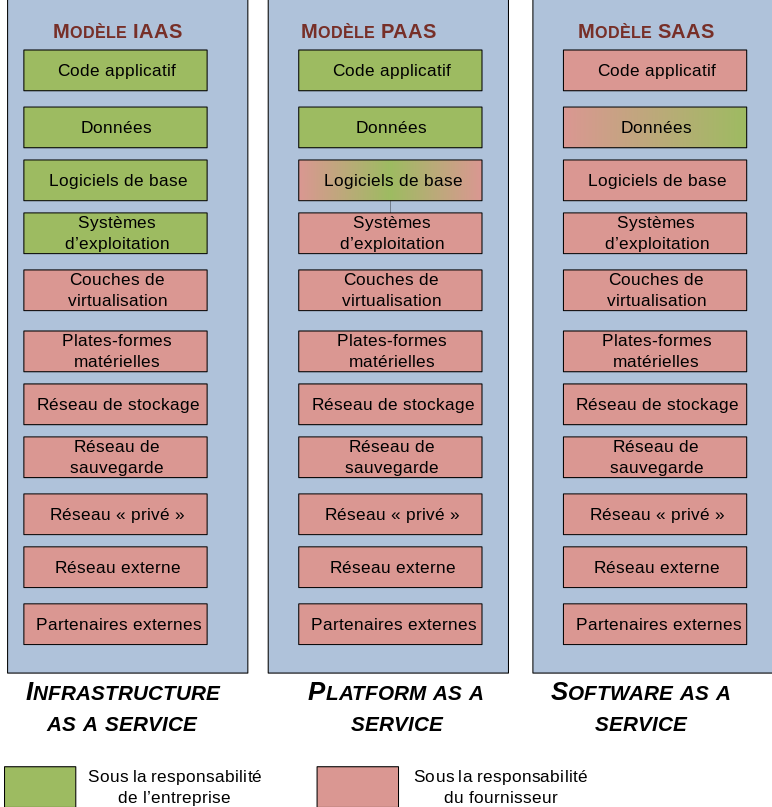
\includegraphics[scale=0.7]{servicesCloud.jpg}
	\caption{Les services du Cloud Computing}
	\label{Les services du Cloud Computing}
\end{figure}
\begin{itemize}
	\item   \textbf{Software-as-a-service} (SAAS): Des applications, aux abonnements, installées ou accessibles via un navigateur. En profitant de ce type de service les fournisseurs gèrent de manière transparente l'ensemble des aspects techniques de l'application. Quant aux clients, ils se limitent à effectuer quelques paramétrages de l'application. 
	\item \textbf{Plateform-as-a-service} (PAAS): Des plateformes de développement ou de test dont le système d'exploitation et les outils sont gérés par les fournisseurs du Cloud. Or les clients gardent la main sur l'installation des applications et leurs paramétrages.
	\item   \textbf{Infrastucture-as-a-service} (IAAS): Les fournisseurs offrent des ressources informatiques  virtualisées (stockage, réseaux, virtualisation, etc.) sur lesquelles le consommateur garde le contrôle sur le système d'exploitation, les applications déployées  et certains composants de réseau. 	Les domaines d'exploitation des infrastructures sont divers, Ils peuvent être  utilisées  comme un réseau privé virtuel dans les entreprises ou pour héberger des sites sur des serveurs virtuels ou pour l'utilisation des data centers virtuels. 
	
\end{itemize}
Ces services peuvent être déployer sur différents modes : \begin{itemize}
	\item \textbf{Cloud privé} : C'est un modèle très répandu dédié à une seule entreprise. Le déploiement de ce dernier peut se faire sous deux autres formats possibles:
	\begin{itemize}
		\item {Cloud privé internalisé}: Dans ce cas, le Cloud est interne à l'entreprise ou entièrement dédié à cette même entreprise. Il est accessible via des réseaux sécurisés et opérés par les équipes internes.
		\item {Cloud privé externalisé}: Dans ce cas, le Cloud offre des services similaires au Cloud privé internalisé. Ce dernier est entièrement dédié à l'entreprise, mais hébergé chez un tiers.
	\end{itemize}
	\item \textbf{Cloud public}: Dans ce cas, le Cloud est externe à l'entreprise et géré par un opérateur externe propriétaire des infrastructures, avec des ressources totalement partagées entre tous ses clients.
	\item \textbf{Cloud hybride}: Dans ce cas, il s'agit de l'association de deux ou plusieurs modèles de cloud pour assurer une portabilité des applications et des données.
\end{itemize}
Bien que le marché du Cloud public est plein de fournisseurs, la concurrence est toujours concentrée entre Amazaon Web Services, Microsoft Azure et Google Cloud Plateform. 
Pour des raisons d'efficacité et de disponibilité, le choix de fournisseur pour Tritux a été fixé sur Google Cloud Plateform.
\subsection{Google Cloud plateform}
La plateforme Cloud de Google (GCP) est un ensemble de ressources informatiques, mises à la disposition du grand public via des services modulaires basés sur le Cloud, sous la forme d'une offre de cloud public.\\
Celle-ci propose des services de calcul, stockage, apprentissage automatique et d'internet des objets, ainsi que des outils de gestion et de sécurité. Les principaux produits de Cloud computing de Google Cloud Platform sont répartis en trois grandes familles:
\begin{itemize}
	\item \textbf{Google App Engine}:  Un  service  Cloud  de  type  PAAS  permet  aux  développeurs 
	d'accéder  à  l'hébergement  évolutif  de  Google.  Les  développeurs  peuvent  également 
	utiliser  un  kit  de  développement  logiciel  pour  implémenter  des  produits  logiciels 
	s'exécutant  sur  App  Engine. 
	\item \textbf{Google Storage}:Une  plateforme  de  stockage   conçue  pour  stocker  des 
	Données de taille importante.
	
	\item \textbf{Google Compute Engine}: Une offre IaaS qui permet aux clients d'exécuter des charges de travail sur le matériel physique de Google.
Il fournit un nombre évolutif de machines virtuelles (VM) pouvant servir de grands clusters de calcul à cette fin.  Google Compute Engine peut être géré via une API REST, une interface de ligne de commande (CLI) ou une console Web. Compute Engine est un service à la carte avec un minimum de 10 minutes.\\
Ainsi ces ressources virtuelles devront être  instanciées, allouées et orchestrées via des plateformes d'administration et de gestion des ressources Cloud.
\end{itemize}

\section{Méthodologie de gestion de  travail }
Dans le processus de réalisation d'un projet complexe, l'utilisation d'une méthodologie de 
management  de  projet  est  indispensable  afin  d'assurer  la  réussite  de  ce  dernier.  En  e?et, 
une  bonne  méthodologie  de  projet  fournit  le  cadre,  les  procédés,  les  lignes  directrices  et 
les  techniques  pour  gérer  à  la  fois  le personnel  et  le  travail. 
.\newline
Il existe  de  nombreuses  méthodologies  de  gestion  de  projet,  assez  différente  les  unes  des 
autres  de  par  leurs  fonctionnements,  mais  ils  se  rejoignent  tous  afin  de  garantir  le  succès 
de  la  conduite  du  projet. \newline
Pour notre projet nous avons opté pour une méthode agile qui permet de se focaliser sur la valeur métier du livrable, d'améliorer constamment la qualité de ce que nous réalisons et de réagir efficacement aux changements.
De ce fait, nous allons donner tout d'abord un aperçu sur les méthodologies agiles. Puis, nous focalisons sur la méthodologie Scrum, qui a été utilisée dans le présent projet.
\subsection{Méthodes Agiles}
Les besoins, dans une équipe de développement logiciel qui travaille sur un projet interne sont parfois susceptibles d'être changés ou modifiés. De ce fait, l'équipe se trouve
en train de développer une application avec des spécifications parfois non précises, ce qui
peut entraîner des retards dans le déploiement du projet. Ces problématiques ont poussé
les ingénieurs à réinventer les méthodes de gestion de projet et de conception en introduisant ce que nous appelons la méthode Agile.
\subsection{Presentation de la méthodologie Scrum}
Scrum est la méthodologie suivie par la société TRITUX pour la gestion de ses projets. C'est une méthodologie agile itérative basée sur des itérations d'une durée de 2 à 4 semaines appelées Sprints.
Durant chacune de ces itérations, une partie du produit nommée .« Incrément » est réalisée en se basant sur les parties crées lors des itérations précédentes et livrées à la fin du Sprint.

Elle  offre les avantages suivants : \begin{itemize}
	\item Flexibilité. 
	\item Pas de distinction des rôles au sein d'une équipe « Scrum ». 
	\item Auto confiance au sein de l'équipe en l'isolant durant le Sprint et en la rendant autogérée. 
	\item Équipes soudées. 
	
\end{itemize}

Il existe différents rôles participants dans la mise en \oe{}uvre

 du projet selon la logique de Scrum: 
\begin{itemize}
	\item \textbf {Product Owner } : C'est un membre à part entière de l'équipe Scrum dont la responsabilité principale est de définir un produit qui apportera le maximum de valeur métier aux utilisateurs dans le temps et le budget. Il présente les besoins du client et propose de nouveaux objectifs. Il contrôle aussi la qualité et la date de délivrance de chaque sprint 
	\item \textbf  {Scrum Master }: Il aide  l'équipe à travailler de façon autonome et à s'améliorer constamment. Il est le garant de l'application du processus, Scrum en l'occurrence. 
	\item \textbf { Scrum Team}: L'équipe de développement 
\end{itemize}

Les artéfacts de cette méthodologie sont de deux types: \cite {ref3}

	\begin{enumerate}
		\item \textbf {Backlog produit }: liste ordonnée de tout ce qui pourrait être requis dans le produit et elle est l'unique source des besoins pour tous les changements à effectuer sur le produit sous la responsabilité du Product Owner. 
			\item \textbf {Backlog sprint }: est constitué à partir des thèmes du Backlog produit. Lors de la réunion de planification de sprint, l'équipe de développement choisit les éléments du Backlog produit qui seront réalisés. Il est sous la responsabilité de l'équipe et elle est seule à pouvoir le modifier en cours d'itération. 
	\end{enumerate}



\section{Conclusion}
 Ce chapitre nous a permis d'introduire notre projet, de présenter l'organisme d'accueil  et  la problématique qui nous suscite à la réalisation de ce projet, ainsi que la solution proposée. Notre rapport sera organisé en respectant les normes de la méthode Agile SCRUM.
En vue de mieux comprendre le métier, une description de l'environnement fera l'objet
du prochain chapitre.

\chapter{Sprint0: Analyse et conception globales }


\section{Introduction}
Ce chapitre sera dédié à l'analyse et à la spécification des besoins. 
En premier lieu, nous identifierons les acteurs principaux du projet. En second lieu, nous définirons les différents besoins fonctionnels et non fonctionnels de notre application. 
Par la suite, nous présenterons une étude conceptuelle globale. Enfin, nous clôturons par définir l'architecture utilisée.


\section{Identification des acteurs}
Un acteur présente une personne, une entité ou un système  agissant d'une façon directe sur l'application.\\
Les différents acteurs modélisant notre système sont :
\begin{itemize}
	\item  \textit{Utilisateur} : un employé de l'entreprise qui peut gérer son profil, consulter ses instances, gérer les planifications, etc.
	\item  \textit{Chef de projet}  est un membre de la société, qui peut en plus des fonctionnalités récemment citées créer de nouvelle instance cloud, gérer des membres de son projet, etc.
	\item  \textit{Administrateur}  directeur technique de l'entreprise et la personne la plus privilégiée, il possède le droit de manipuler toutes les fonctionnalités offertes par notre application.
\end{itemize}
L'ensemble de ces acteurs sont liées par une relation d'héritage. 
\section{Identification des besoins}
Dans cette section, nous allons développer les besoins fonctionnels et non fonctionnels de l'entreprise d'accueil.
\subsection{Besoins fonctionnels}
Les besoins fonctionnels expriment les principales fonctionnalités de l'application sans se
préoccuper de la façon de l'implémentation.\\
Une étude détaillée de système nous a permis de dégager les principaux exigences fonctionnelles
des différents acteurs de notre application.
\begin{itemize}
	\item Authentification et gestion de mot de passe.
	\item Consultation et modification du profil.
	\item Gestion des projets notamment création, suppression et modification.
	\item Gestion des utilisateurs qui contient le volet de consultation et de suppression.
		\item Gestion des planifications notamment création et suppression.
	\item Affectation/ retrait d'un projet à un utilisateur.
	\item Affectation/retrait d'un planning des instances de machines virtuelles.
	\item Manipulation des instances de machine virtuelle. Un utilisateur peut consulter, activer, arrêter 
	une instance.
	\item Attribution des droits d'accès différents selon l'utilisateur.
	\item Gestion des machines virtuelles.
	\item Gestion des instances de machine virtuelle qui contient le volet de création et de suppression réalisée que par le chef de projet et l'administrateur.
\end{itemize}


\subsection{Besoins non fonctionnels}
Pour garantir un bon fonctionnement de l'application, cette dernière doit assurer les besoins non fonctionnels présentés ci-dessous.
\begin{itemize}
	\item Ergonomie : Les interfaces doivent être conviviales, ergonomiques et facile à exploiter par l'utilisateur.
	\item Fiabilité : L'application doit fournir des résultats correctes.
	\item Sécurité : L'accès à l'application ainsi qu'aux données doit être sécurisé. D'une part par
	la gestion des autorisations aux différents modules de l'application grâces aux privilèges
	gérés par le module d'administration et d'une autre part par l'intégration d'un module
	d'authentification basée sur l'échange de jetons  entre le serveur et le client.
	\item Extensibilité : Le système doit être extensible et permet de s'intégrer facilement sur le réseau existant  de l'entreprise. Il doit aussi supporter l'intégration d'autres fonctionnalités
	\item  Maintenabilité : La maintenabilité et l'évolutivité sont des priorités. Le code sera lisible,
	commenté, divisé en fonction des pages (des interfaces) et en fonction des tâches abordées.

\end{itemize}
\section{Étude conceptuelle}

Nous allons exposer dans cette section le diagramme de cas d'utilisation et de classe globales modélisant notre projet.

\subsection {Diagramme de cas d'utilisation global }
Dans cette partie, nous présentons le diagramme de cas d'utilisation global qui modélise
l'interaction entre le système informatique à développer et les acteurs interagissant avec le système.
Également, il permet de recenser  les besoins des utilisateurs et les fonctionnalités du système.
\newpage
\begin{figure}[H]
	\centering
	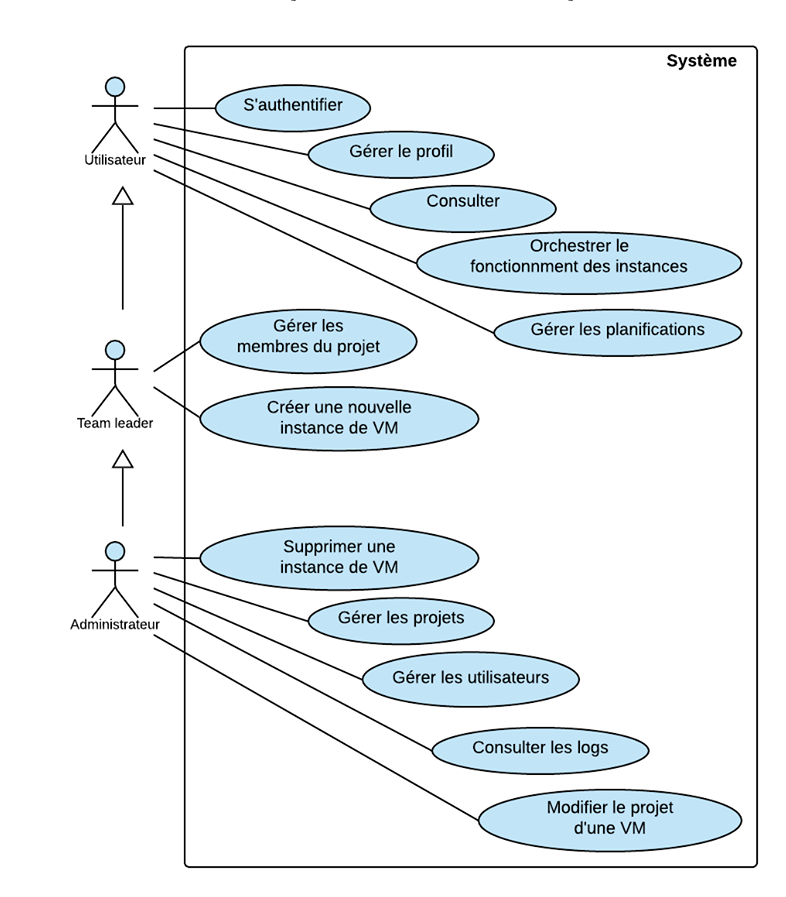
\includegraphics[scale=0.5]{DCUglobal.png}
	\caption{Diagramme de cas d'utilisation global}
	\label{Diagramme de cas d'utilisation global}
\end{figure}
 La figure 2.1 ci-dessus représente le diagramme de cas d'utilisation global de notre
projet où on y trouve les acteurs principaux et leurs rôles.\\ Ce diagramme décrit de manière globale les différentes fonctionnalités de chaque acteur. 
En effet, tout utilisateur est apte à s'authentifier, gérer son profil, consulter les projets,  gérer les planifications de fonctionnement des machines virtuelles et orchestrer leurs fonctionnements.
Notre deuxième acteur est un Team leader qui est utilisateur privilégié par la gestion des membres du projet et la création des machines virtuelles.
De plus que les fonctionnalités de Team leader et d'utilisateur, l'administrateur assure la gestion des utilisateurs et la consultation des logs.
\section{Étude conceptuelle globale}
\subsection{Diagramme de classe global}
Le diagramme de classe  est considéré parmi les diagrammes les plus importants dans la modélisation  de l'UML(Unified Modeling Language), comme présenté dans la figure 2.2, il permet de décrire la structure statique d'un système en présentant ses différents classes, attributs, méthodes et relations entre ses objets. 

\begin{figure}[H]
	\centering

	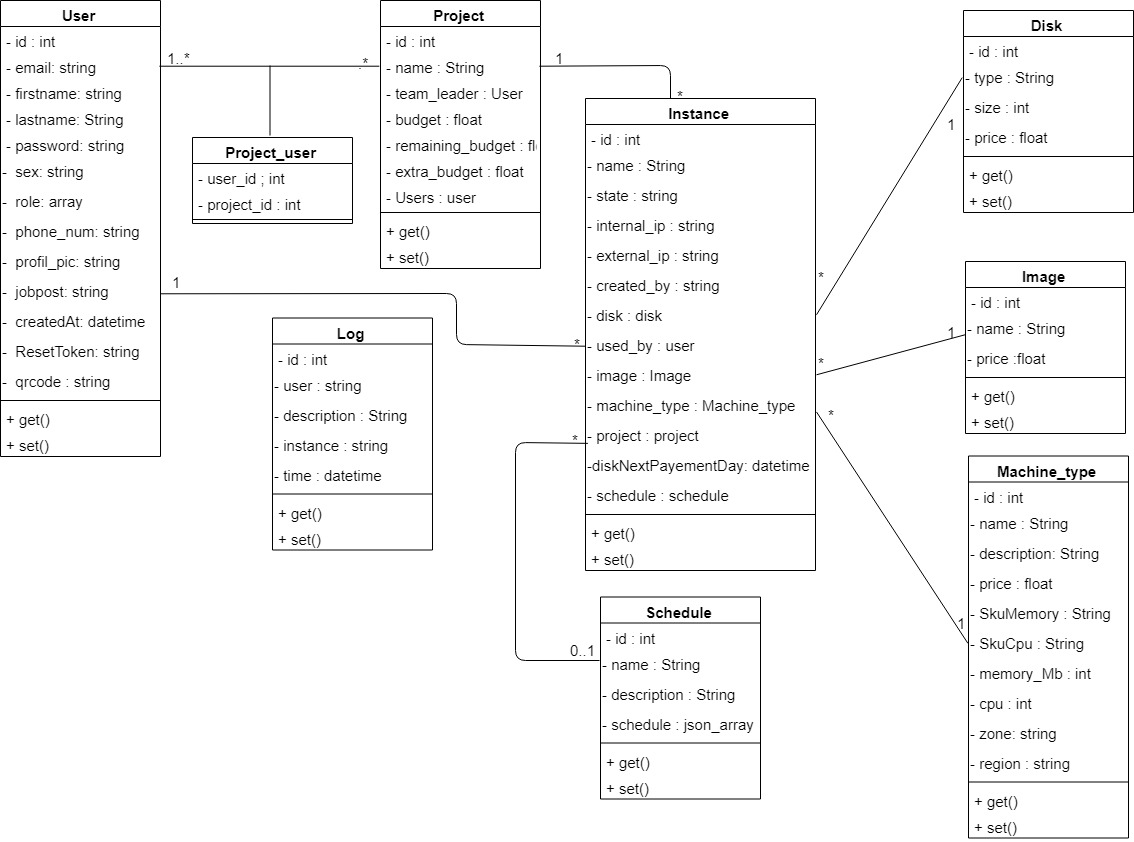
\includegraphics[ height=16cm, width=16cm]{diagdeclass.jpg}
	\caption{Diagramme de classe global}
	\label{Diagramme de classe global}
\end{figure}

\section{Spécifités techniques}
\subsection{Backlog produit}
Le Backlog est un artéfact très important dans Scrum. C'est l'ensemble des
caractéristiques fonctionnelles ou techniques qui constituent le produit souhaité.
Le tableau 2.1 résume le backlog produit de notre application où chaque user story est
caractérisé par un identifiant, un nom et une estimation.

% Please add the following required packages to your document preamble:
% \usepackage{multirow}
\begin{table}[H]
	\begin{tabular}{|l|l|l|l|}
		\hline
		\textbf{ID}        & \textbf{Tâches}                             & \textbf{User Story}                                                                                                                                       & \textbf{Esti.} \\ \hline
		\multirow{5}{*}{1} & \multirow{5}{*}{Gestion des comptes}        & \begin{tabular}[c]{@{}l@{}}1.1 En tant que utilisateur, je souhaite \\ m'inscrire à l'application.\end{tabular}                                           & 3              \\ \cline{3-4} 
		&                                             & \begin{tabular}[c]{@{}l@{}}1.2 En tant que utilisateur, je souhaite\\ m'authentifier à l'application.\end{tabular}                                        & 5              \\ \cline{3-4} 
		&                                             & \begin{tabular}[c]{@{}l@{}}1.3 En tant que utilisateur je souhaite \\ recevoir un mail de réinitialisation du mot\\ de passe en cas d'oubli.\end{tabular} & 5              \\ \cline{3-4} 
		&                                             & \begin{tabular}[c]{@{}l@{}}1.4 En tant que utilisateur, je souhaite\\ consulter mon profil.\end{tabular}                                                  & 3              \\ \cline{3-4} 
		&                                             & \begin{tabular}[c]{@{}l@{}}1.5 En tant que utilisateur, je souhaite \\ mettre à jour mes données personnelles.\end{tabular}                               & 3              \\ \hline
		\multirow{4}{*}{2} & \multirow{4}{*}{Gestion des utilisateurs}   & \begin{tabular}[c]{@{}l@{}}2.1 En tant que administrateur, je souhaite\\ consulter la liste des utilisateurs de \\ l'application\end{tabular}             & 2              \\ \cline{3-4} 
		&                                             & \begin{tabular}[c]{@{}l@{}}2.2 En tant que administrateur, je souhaite\\ supprimer un utilisateur.\end{tabular}                                           & 2              \\ \cline{3-4} 
		&                                             & \begin{tabular}[c]{@{}l@{}}2.3 En tant que administrateur, je souhaite\\ affecter un projet à un utilisateur.\end{tabular}                                & 3              \\ \cline{3-4} 
		&                                             & \begin{tabular}[c]{@{}l@{}}2.4 En tant que administrateur, je souhaite\\ retirer un projet d'un utilisateur.\end{tabular}                                 & 3              \\ \hline
		\multirow{6}{*}{3} & \multirow{6}{*}{Management des projets}     & \begin{tabular}[c]{@{}l@{}}3.1 En tant que Team leader, je souhaite\\ consulter mes projets.\end{tabular}                                                 & 2              \\ \cline{3-4} 
		&                                             & \begin{tabular}[c]{@{}l@{}}3.2 En tant que administrateur, je souhaite\\ supprimer un projet.\end{tabular}                                                & 2              \\ \cline{3-4} 
		&                                             & \begin{tabular}[c]{@{}l@{}}3.3 En tant que administrateur, je souhaite \\ créer un projet.\end{tabular}                                                   & 2              \\ \cline{3-4} 
		&                                             & \begin{tabular}[c]{@{}l@{}}3.4 En tant que administrateur, je souhaite\\ modifier un projet.\end{tabular}                                                 & 2              \\ \cline{3-4} 
		&                                             & \begin{tabular}[c]{@{}l@{}}3.5 En tant que Team leader, je souhaite \\ ajouter un membre à mon projet.\end{tabular}                                       & 3              \\ \cline{3-4} 
		&                                             & \begin{tabular}[c]{@{}l@{}}3.6 En tant que Team leader, je souhaite \\ retirer un membre de mon projet.\end{tabular}                                      & 3              \\ \hline
		\multirow{5}{*}{4} & \multirow{5}{*}{Management des VMs}         & \begin{tabular}[c]{@{}l@{}}4.1 En tant que utilisateur je souhaite \\ consulter la liste des VMs.\end{tabular}                                            & 5              \\ \cline{3-4} 
		&                                             & \begin{tabular}[c]{@{}l@{}}4.2 En tant que utilisateur je souhaite \\ orchestrer le fonctionnement des VMs.\end{tabular}                                  & 5              \\ \cline{3-4} 
		&                                             & \begin{tabular}[c]{@{}l@{}}4.3 En tant que Team leader je souhaite créer\\ de nouvelles instances de machine \\ virtuelle.\end{tabular}                   & 7              \\ \cline{3-4} 
		&                                             & \begin{tabular}[c]{@{}l@{}}4.4 En tant que administrateur, je souhaite\\ supprimer  une machine virtuelle.\end{tabular}                                   & 7              \\ \cline{3-4} 
		&                                             & \begin{tabular}[c]{@{}l@{}}4.5 En tant que administrateur, je souhaite\\ modifier le projet d'une machine virtuelle.\end{tabular}                         & 3              \\ \hline
		\end{tabular}
\end{table}

\begin{table}[H]
	\begin{tabular}{|l|l|l|l|}
		\hline
		\textbf{ID}        & \textbf{Tâches}                             & \textbf{User Story}                                                                                                                                       & \textbf{Esti.} \\ \hline
	\multirow{5}{*}{5} & \multirow{5}{*}{Gestion des planifications} & \begin{tabular}[c]{@{}l@{}}5.1 En tant que utilisateur, je souhaite \\ consulter la liste des plannings.\end{tabular}                                     & 2              \\ \cline{3-4} 
&                                             & \begin{tabular}[c]{@{}l@{}}5.2 En tant que utilisateur, je souhaite créer \\ un planning.\end{tabular}                                                    & 4              \\ \cline{3-4} 
&                                             & \begin{tabular}[c]{@{}l@{}}5.3 En tant que utilisateur,je souhaite \\ supprimer un planning.\end{tabular}                                                 & 3              \\ \cline{3-4} 
&                                             & \begin{tabular}[c]{@{}l@{}}5.4 En tant que utilisateur, je souhaite affecter\\ un planning à une VM.\end{tabular}                                         & 5              \\ \cline{3-4} 
&                                             & \begin{tabular}[c]{@{}l@{}}5.5 En tant que utilisateur, je souhaite retirer\\ un planning d'une VM.\end{tabular}                                          & 3              \\ \hline
6                  & Gestion des logs                            & \begin{tabular}[c]{@{}l@{}}6.1 En tant que utilisateur, je souhaite \\ consulter les activités des utilisateurs.\end{tabular}                             & 3              \\ \hline

	\end{tabular}
\caption{Backlog produit}
\label{Backlog produit}
\end{table}

\subsection{Planification du projet}
La planification de notre projet est résumée par  la figure 2.3
\begin{figure}[h]
	\centering
	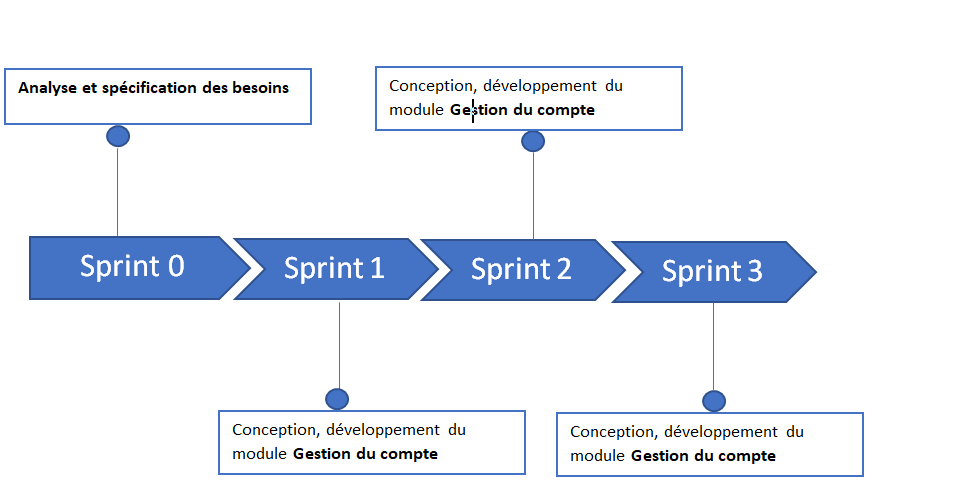
\includegraphics[scale=0.5]{decoupageSprint.PNG}
	\caption{Découpage du projet}
	\label{Découpage du projet}
\end{figure}
\begin{itemize}
	\item \textbf{Sprint 0}: contient une étude préalable du projet.
	\item \textbf{Sprint 1}: \begin{itemize}
		\item Gestion des comptes: contient toutes les fonctionnalités liées à l'accès à l'application et le contrôle des données personnelles.
		\item Gestion des utilisateurs: contient les fonctionnalités liées au contrôle des utilisateurs.

	\end{itemize}  .
\item \textbf{Sprint 2}: 
\begin{itemize}
	\item Management des projets: contient les fonctionnalités liées à la gestion des projets de Tritux.
	\item Management des ressources Cloud: contient les fonctionnalités liées aux contrôle et gestion des ressources Cloud.
\end{itemize}
\item \textbf{Sprint 3}:
\begin{itemize}
	\item Gestion des Planifications.
    \item Gestion des logs

\end{itemize}
\end{itemize}
\subsection{Environnement de travail}
La réussite  de notre travail dépend énormément du choix des technologies et outils utilisés tout en tenant compte du besoin de l'entreprise.
\subsubsection{Choix techniques  pour le Front-end}
\textbf{Angular 7}\\
Angular 7 est la version la plus récente du framework open source Angular, lancé le 18 octobre 2018 par Google. Ce dernier est un framework modulaire à base de components et modules. Il assure 
la création des applications mono-pages (SPA : Signle Page Application), web et mobiles. 
\\ 
Angular 7 propose plusieurs fonctionnalités parmi eux: 
\begin{itemize}
	\item Pipe: Composant permettant la transformation et la personnalisation de l'affichage des données  dans les balises HTML.
	\item Vue: Des fichiers de HTML5 et CSS3.
	\begin{itemize}
		\item  HTML5: Le standard HTML est l'acronyme de « HyperText Mark-Up Language », c'est un
		langage de balisage développé pour la formalisation de l'écriture d'un document. 
		\item CSS3: 
	Les feuilles de styles  sont un langage qui
	permet de gérer la présentation et la mise en forme d'une page web.	
	
	\end{itemize}
	\item Contrôleur: Classe TypeScript représente la logique de la vue. Elle traite les différentes taches à réaliser. Ainsi elle fait le lien entre la vue et les services en invoquant ses méthodes.
	\begin{itemize}
		\item TypeScript: Langage de programmation open-source développé par Microsoft. Il s'agit d'un sur-ensemble syntaxique strict de JavaScript, qui ajoute un typage statique optionnel au langage. TypeScript tend à améliorer et à sécuriser la production du
		code JavaScript.
	\end{itemize}
	\item Services: Composant assurant l'émission, le traitement et la réception des requêtes http, en vue  d'assurer l'échange des données JSON entre les services Web et le contrôleur.
	\begin{itemize}
		\item 
		JSON: JavaScript Object Notation est un format d'échange de données léger. Ainsi, Il est facile pour la lecture et écriture des données. Basé sur le Javascript, le JSON est un format de texte totalement indépendant du langage, c'est-à-dire, il permet de faire communiquer deux langages de programmation différents.
	\end{itemize}
\end{itemize}

\begin{table}[H]  
	

	\begin{tabular}{|l|l|l|l|}
		\hline
		\textbf{Framework}                                                           & \textbf{ReactJS}                                                                                                                             & \textbf{Angular}                                                          & \textbf{Vue}                                                                                                                                  \\ \hline
		\textbf{\begin{tabular}[c]{@{}l@{}}Courbe \\ d'apprentissage\end{tabular}}   & Difficile                                                                                                                                    & Moyen                                                                     & Facile                                                                                                                                        \\ \hline
		\textbf{Scalabilité}                                                         & Haute                                                                                                                                        & Haute                                                                     & Faible                                                                                                                                        \\ \hline
		\textbf{\begin{tabular}[c]{@{}l@{}}Communauté et \\ popularité\end{tabular}} & \begin{tabular}[c]{@{}l@{}}Le plus populaire,\\  entrain de devenir \\ un bon choix pour \\ les applications\\  mobiles natives\end{tabular} & \begin{tabular}[c]{@{}l@{}}Il se développe \\ tellement vite\end{tabular} & \begin{tabular}[c]{@{}l@{}}Une communauté très\\  active et entrain de se\\  développer\end{tabular}                                          \\ \hline
		\textbf{Emplois}                                                             & Fortement demandé                                                                                                                            & \begin{tabular}[c]{@{}l@{}}Fortement\\  demandé\end{tabular}              & \begin{tabular}[c]{@{}l@{}}Moins populaire et \\ n'est pas supporté \\ par une grande \\ entreprise comme \\ Facebook ou Google.\end{tabular} \\ \hline
		\textbf{Performance}                                                         & Haute                                                                                                                                        & moyenne                                                                   & Haute                                                                                                                                         \\ \hline
	\end{tabular}
	\caption{Comparaison des Frameworks les plus populaires du Front-end}
\label{Comparaison des Frameworks les plus populaires du Front-end}
\end{table}
En se basant sur le tableau comparatif 2.2, le choix
du Framework à utiliser a été fixé sur Angular 7 puisqu'il répond parfaitement à nos besoins et aux
exigences techniques du développement de notre application.
\title {Symfony}
\subsubsection{Choix techniques pour le Back-end}
\textbf{Symfony 4} \\
Symfony est un puissant Framework de PHP qui permet de réaliser des sites complexes rapidement, mais de façon structurée et avec un code clair, maintenable et sécurisé en respectant les normes
de programmation. Ainsi Symfony bénéficie d'une richesse des bundles (plugins) développés et permettent de séparer la partie métier de la partie données. Ce dernier est utilisé par Tritux pour la plupart des projets web.\\

\subsubsection{Outils}
\begin{itemize}
\item 	\textbf{Cron job} \newline
	Cron est un utilitaire qui planifie l'exécution automatique d'une commande ou d'un script sur le serveur  à des temps prédéfinis ou après certains intervalles prédéfinis. Un travail cron est la tâche planifiée elle-même. Les tâches Cron peuvent être très utiles pour automatiser des tâches répétitives tels que le contrôle  du budget restant du projet et l'automatisation du fonctionnement des VMs.
	\item \textbf{Node.js} \\Node est une plateforme de développement open source permettant d'exécuter du code JavaScript côté serveur. Node est utile pour développer des applications nécessitant une connexion persistante du navigateur au serveur et exécutant sur un serveur HTTP dédié.
	\begin{figure}[H]
		\centering
		
\includegraphics[scale=0.05]{node.png}
		\caption{Logo Nodejs}
		\label{Logo Nodejs}
	\end{figure} 
\item 
\textbf{Git} \\ Git est un système de contrôle de version distribué gratuit et à source ouverte, conçu pour gérer tout projet, du plus petit au plus grand, avec rapidité et efficacité.
	\begin{figure}[H]
	\centering
	
\includegraphics[scale=0.2]{git.png}
	\caption{Logo Git}
	\label{Logo Git}
\end{figure} 
\item \textbf{Postman} \\ Postman est un puissant client HTTP pour tester les services Web, il facilite le test, le développement et la documentation des API en permettant aux utilisateurs de créer rapidement des requêtes HTTP simples et complexes.
	\begin{figure}[H]
	\centering
	
\includegraphics[scale=0.7]{postman.png}
	\caption{Logo Postman}
	\label{Logo Postman}
\end{figure} 

\end{itemize}

\section{Architecture de l'application}
\subsection{Architecture physique de l'application}
Notre application respecte la logique de l'architecture 3-tiers : nous avons un serveur pour la
Base de données, un serveur Web pour recevoir et émettre les requêtes du client et un serveur client.
	\begin{figure}[h]
	\centering
	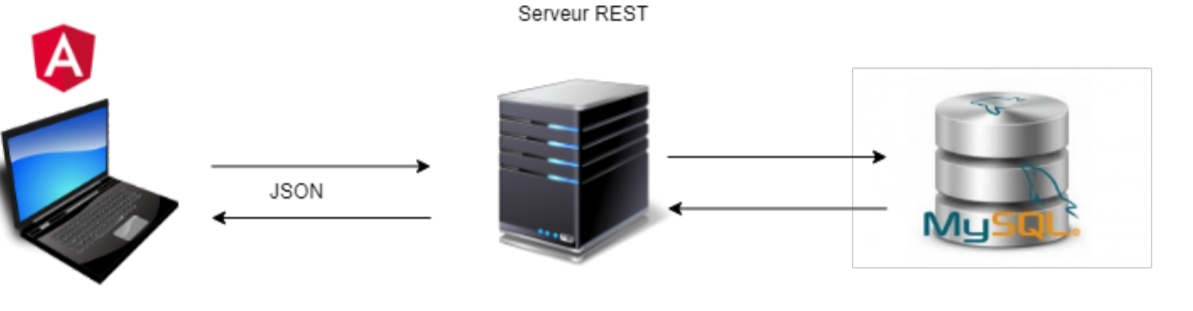
\includegraphics[scale=0.5]{archiphy.PNG}
	\caption{Architecture physique de l'application}
	\label{Architecture physique de l'application}
\end{figure} 
\begin{itemize}
	\item Couche de présentation: Elle correspond à la partie visible et interactive de l'application
	pour les utilisateurs.
	\item Couche de logique métier: Elle permet d'appliquer les règles du métier gérées par
	l'application. Elle agit sur les données capturées à partir de la couche d'accès des données.
	\item Couche d'accès aux données: Elle correspond aux données qui sont destinées à être conservées.
\end{itemize}
La communication entre le client et le serveur REST est assurée par le biais d'échange des APIs REST.
\subsubsection{API REST}
REST est une API qui utilise les méthodes HTTP pour accéder à des ressources
distantes sur le web. Chaque ressource est représentée par une URI 6 qui permet d'avoir
un système universel d'identification des éléments de l'application. Elle supporte plusieurs
formats de données comme JSON, XML, YML.
\subsection {Architecture logique de l'application}

\subsubsection{Architecture Front-end}


	\begin{figure}[h]
	\centering
	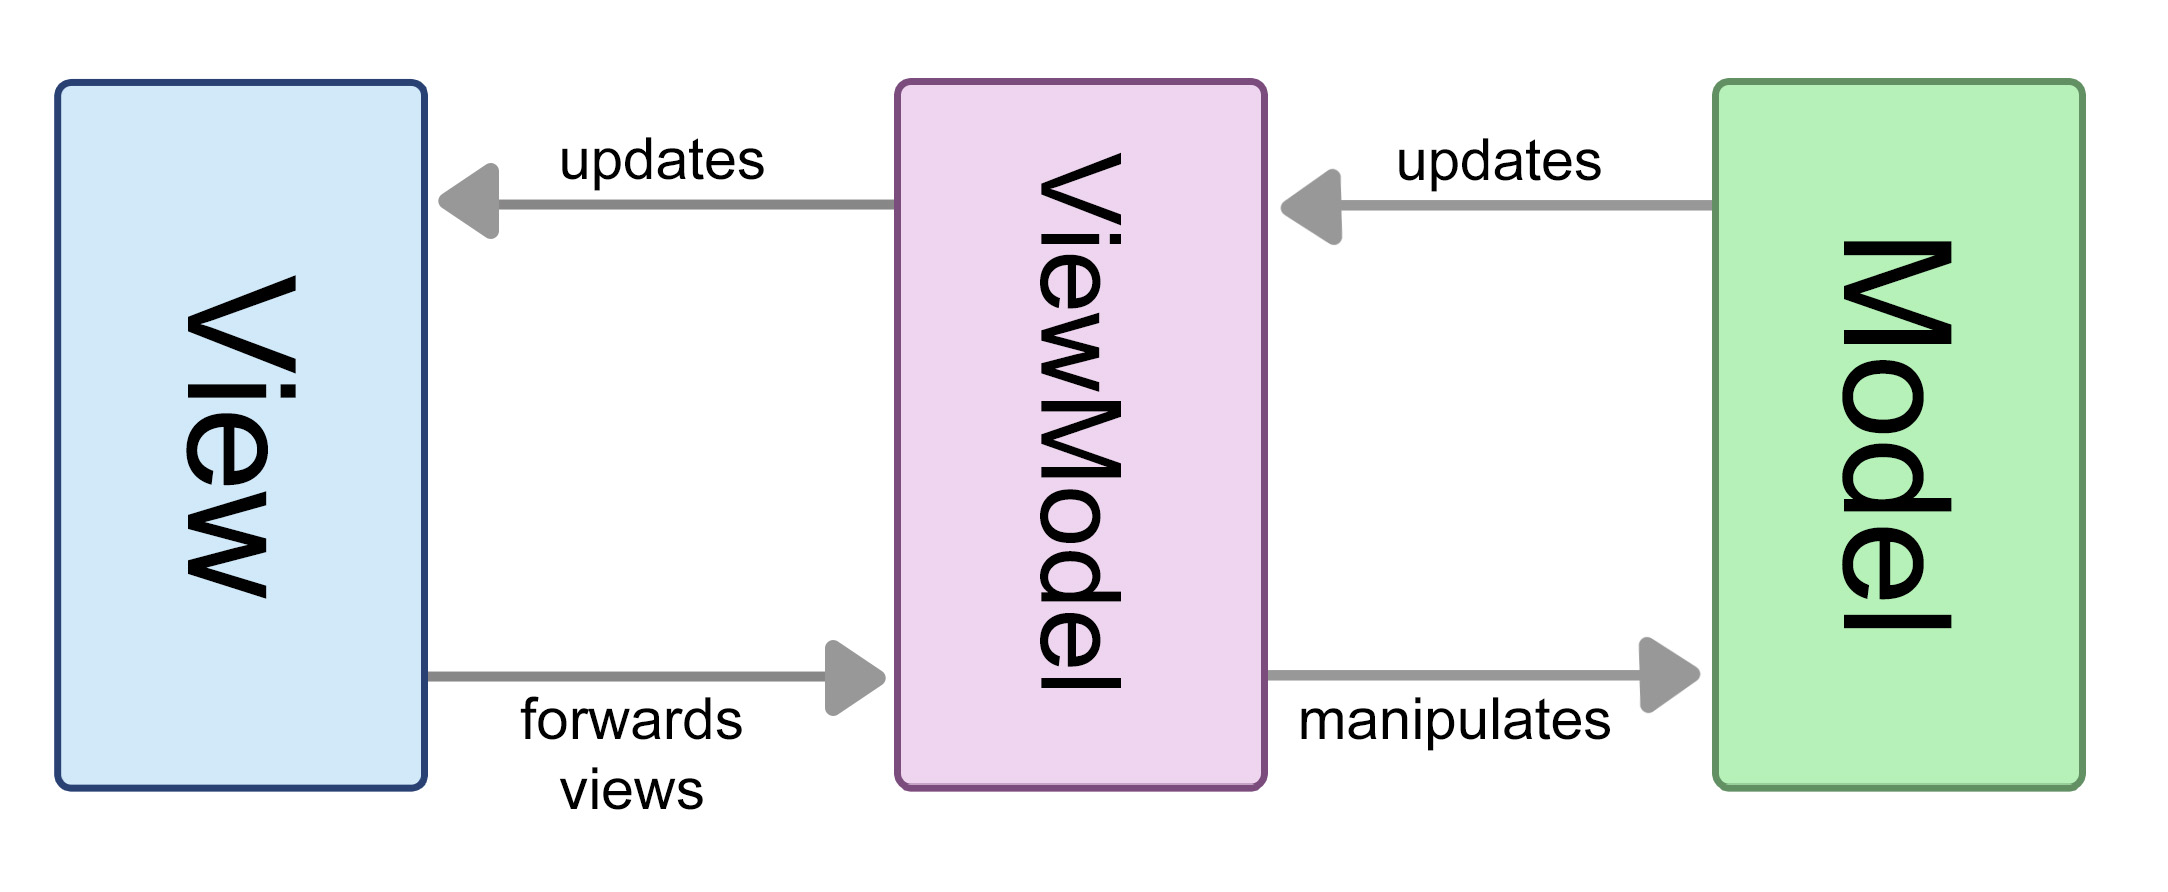
\includegraphics[scale=0.1]{mvvm.jpg}
	\caption{Architecture logique Front-end de l'application}
	\label{Architecture logique Front-end de l'application}
\end{figure} 
MVVM pour model view view-Model est un design pattern qui facilite la séparation du développement de l'interface utilisateur, c'est-à-dire de la couche de présentation.\\Comme le montre la figure 2.12  ViewModel (VM) est chargé d'exposer les objets de données du modèle de manière à ce que les objets soient plus facilement gérés et présentés.\\
Pour son architecture, Angular adopte le modèle MVVM, cette implémentation est présentée comme suit : 
%il faut verifier l'architecture logique d'angular
\begin{itemize}
	\item \textit{Model}  est implémenté en tant que service angulaire.
	\item \textit{View}  est implémentée à l'aide d'un modèle angulaire.
	\item \textit {ViewModel}  est implémenté en tant que contrôleur angulaire. La directive 'ngController' permet de spécifier un contrôleur pour une vue.
\end{itemize}
\subsubsection{Architecture Back-end}

Symfony est basée sur l'architecture MVC (modèle, vue et contrôleur) qui est  
un modèle architectural très puissant, il
tire sa puissance de son concept de base qui est la séparation des données (modèle), de
l'affichage (vue) et des actions (contrôleur).
	\begin{figure}[H]
	\centering
	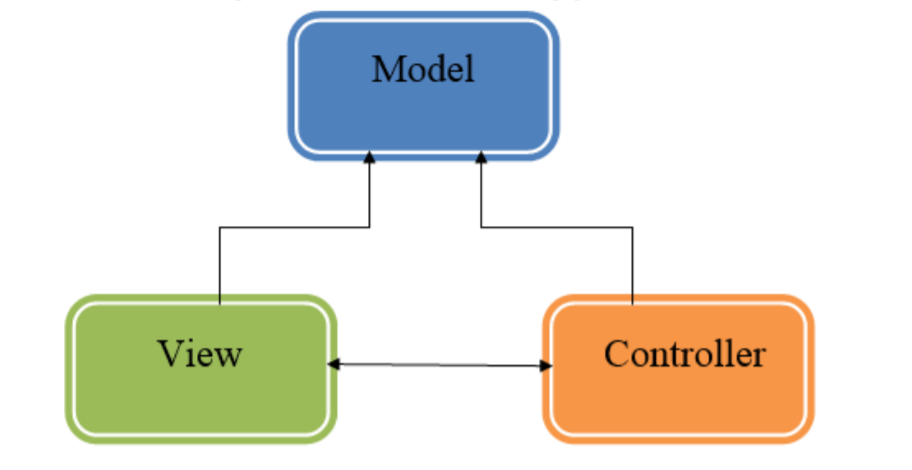
\includegraphics[scale=0.5]{archisym.PNG}
	\caption{Architecture logique Back-end de l'application}
	\label{Architecture logique Back-end de l'application}
\end{figure} 

\section{Conclusion}
Ce chapitre nous a été utile pour montrer notre objectif, nos besoins et éclaircir notre
démarche à travers l'identification des acteurs et des besoins. Il nous a offert une vision plus détaillée en réalisant  une étude conceptuelle globale et en présentant les spécificités techniques de l'application. Le chapitre suivant sera consacré à réaliser le premier incrément de notre projet.
\chapter{Sprint1: Gestion des comptes et des utilisateurs}
\section {Introduction}
L'objectif de ce chapitre est de présenter la première itération du cycle de vie de notre
projet. Nous entamons par identifier les tâches à réaliser dans le Backlog du Sprint pour
passer par la suite aux phases d'analyse et de conception et nous finirons par exposer la phase de
réalisation de ce module.\\
Nous avons découpés ce sprint en deux parties, une pour la gestion des comptes et une autre pour la gestion des utilisateurs.
\section{Étude fonctionnelle} 
\subsection{Backlog du sprint}
Le Backlog du sprint présentés par le tableau 3.1 contient une liste des tâches de chaque user story identifiées par l'équipe Scrum et qui
devront être réalisées pendant ce sprint.
\begin{table}[H]
	\begin{tabular}{|l|l|l|l|}
		\hline
		\textbf{ID}          & \textbf{User Story}                                                                                                                                                     & \textbf{Description}                                                                                                                                                     & \textbf{Esti.} \\ \hline
		\multirow{3}{*}{1.1} & \multirow{3}{*}{\begin{tabular}[c]{@{}l@{}}En tant que utilisateur, je souhaite \\ m'inscrire à l'application.\end{tabular}}                                            & \begin{tabular}[c]{@{}l@{}}Créer la vue d'inscription\\  sécurisée par reCAPTCHA.\end{tabular}                                                                           & 3              \\ \cline{3-4} 
		&                                                                                                                                                                         & \begin{tabular}[c]{@{}l@{}}Générer l'API de création \\ d'un compte\end{tabular}                                                                                         & 3              \\ \cline{3-4} 
		&                                                                                                                                                                         & Consommer l'API                                                                                                                                                          & 3              \\ \hline
			\end{tabular}
	\end{table}


\begin{table}[H]
	\begin{tabular}{|l|l|l|l|}
		\hline
		\textbf{ID}          & \textbf{User Story}                                                                                                                                                     & \textbf{Description}                                                                                                                                                     & \textbf{Esti.} \\ \hline
	
		\multirow{4}{*}{1.2} & \multirow{4}{*}{\begin{tabular}[c]{@{}l@{}}En tant que utilisateur, je souhaite\\ m'authentifier à l'application.\end{tabular}}                                         & Créer la vue d'authentification                                                                                                                                          & 5              \\ \cline{3-4} 
		&                                                                                                                                                                         & \begin{tabular}[c]{@{}l@{}}Créer l'action d'interception \\ de toutes les requetes du \\ front-end et de les  \\ affecter un Bearer Toekn \\ correspondant.\end{tabular} & 4              \\ \cline{3-4} 
		&                                                                                                                                                                         & \begin{tabular}[c]{@{}l@{}}Implémenter l'API \\ d'authentification en\\  émettant le JWT \\ (Json Web Token) vers \\ le front-end\end{tabular}                           & 4              \\ \cline{3-4} 
		&                                                                                                                                                                         & \begin{tabular}[c]{@{}l@{}}Consommer l'API et \\ sauvegarder le token.\end{tabular}                                                                                      & 3              \\ \hline
		\multirow{3}{*}{1.3} & \multirow{3}{*}{\begin{tabular}[c]{@{}l@{}}En tant que utilisateur je souhaite \\ recevoir un mail de réinitialisation \\ du mot de passe en cas d'oubli.\end{tabular}} & \begin{tabular}[c]{@{}l@{}}Créer les vues de saisie\\  du mail et de création \\ d'un nouveau mot de passe.\end{tabular}                                                 & 3              \\ \cline{3-4} 
		&                                                                                                                                                                         & \begin{tabular}[c]{@{}l@{}}Implémenter l'API de \\ réinitialisation du \\ mot de passe.\end{tabular}                                                                     & 5              \\ \cline{3-4} 
		&                                                                                                                                                                         & Consommer l'API.                                                                                                                                                         & 3              \\ \hline
		\multirow{3}{*}{1.4} & \multirow{3}{*}{\begin{tabular}[c]{@{}l@{}}En tant que utilisateur, je souhaite\\ consulter mon profil.\end{tabular}}                                                   & \begin{tabular}[c]{@{}l@{}}Créer la vue de \\ consultation du profil.\end{tabular}                                                                                       & 3              \\ \cline{3-4} 
		&                                                                                                                                                                         & \begin{tabular}[c]{@{}l@{}}Générer l'API permettant \\ de retourner des données\\  d'un utilisateur.\end{tabular}                                                        & 3              \\ \cline{3-4} 
		&                                                                                                                                                                         & Consommer l'API                                                                                                                                                          & 3              \\ \hline
		\multirow{4}{*}{1.5} & \multirow{4}{*}{\begin{tabular}[c]{@{}l@{}}En tant que utilisateur, je souhaite \\ mettre à jour mes données \\ personnelles.\end{tabular}}                             & \begin{tabular}[c]{@{}l@{}}Créer la vue de modification \\ du profil, avec modale de \\ confirmation par mot de \\ passe\end{tabular}                                    & 3              \\ \cline{3-4} 
		&                                                                                                                                                                         & \begin{tabular}[c]{@{}l@{}}Créer l'API de modification\\  du profil.\end{tabular}                                                                                        & 3              \\ \cline{3-4} 
		&                                                                                                                                                                         & \begin{tabular}[c]{@{}l@{}}Créer l'API de confirmation \\ du modification.\end{tabular}                                                                                  & 3              \\ \cline{3-4} 
		&                                                                                                                                                                         & Consommer les deux APIs.                                                                                                                                                 & 3              \\ \hline
			\multirow{3}{*}{2.1} & \multirow{3}{*}{\begin{tabular}[c]{@{}l@{}}En tant que administrateur, je souhaite\\ consulter la liste des utilisateurs de \\ l'application\end{tabular}}              & \begin{tabular}[c]{@{}l@{}}Créer la "datatable" de \\ sélection de tous les \\ utilisateurs.\end{tabular}                                                                & 2              \\ \cline{3-4} 
		&                                                                                                                                                                         & \begin{tabular}[c]{@{}l@{}}Implémenter l'API de\\  sélection des  utilisateurs.\end{tabular}                                                                             & 3              \\ \cline{3-4} 
		&                                                                                                                                                                         & Consommer l'API.                                                                                                                                                         & 3              \\ \hline

\end{tabular}
\end{table}
\begin{table}[H]
	\begin{tabular}{|l|l|l|l|}
		\hline
		\textbf{ID}          & \textbf{User Story}                                                                                                                                                     & \textbf{Description}                                                                                                                                                     & \textbf{Esti.} \\ \hline
	
		\multirow{2}{*}{2.2} & \multirow{2}{*}{\begin{tabular}[c]{@{}l@{}}En tant que administrateur, je souhaite\\ supprimer un utilisateur.\end{tabular}}                                            & \begin{tabular}[c]{@{}l@{}}Implémenter l'API de\\  suppression d'un utilisateur.\end{tabular}                                                                            & 2              \\ \cline{3-4} 
		&                                                                                                                                                                         & Consommer l'API.                                                                                                                                                         & 3              \\ \hline
		\multirow{3}{*}{2.3} & \multirow{3}{*}{\begin{tabular}[c]{@{}l@{}}En tant que administrateur, je souhaite\\ affecter un projet à un utilisateur.\end{tabular}}                                 & \begin{tabular}[c]{@{}l@{}}Créer la modale de \\ consultation,affectation \\ et de détachement des\\  projets d'un utilisateur\end{tabular}                              & 3              \\ \cline{3-4} 
		&                                                                                                                                                                         & \begin{tabular}[c]{@{}l@{}}Implémenter l'API \\ d'affectation d'un projet \\ à un utilisateur.\end{tabular}                                                              & 3              \\ \cline{3-4} 
		&                                                                                                                                                                         & Consommer l'API.                                                                                                                                                         & 3              \\ \hline
		\multirow{2}{*}{2.4} & \multirow{2}{*}{\begin{tabular}[c]{@{}l@{}}En tant que administrateur, je souhaite\\ retirer un projet d'un utilisateur.\end{tabular}}                                  & \begin{tabular}[c]{@{}l@{}}Implémenter l'API de \\ retrait d'un projet de \\ l'utilisateur.\end{tabular}                                                                 & 3              \\ \cline{3-4} 
		&                                                                                                                                                                         & Consommer l'API                                                                                                                                                          & 3              \\ \hline
		
	\end{tabular}

\caption{Backlog du Sprint 1}
\label{Backlog  du Sprint 1}
\end{table}

\subsection{Diagramme de cas d'utilisation du sprint 1}

Le diagramme de cas d'utilisation du premier sprint présenté par la figure 3.1 a pour objectif de déterminer les besoins, les résultats attendus 
et les objectifs les plus prioritaires de la première valeur métier.\\ La détermination des besoins est basée sur la représentation de
l'interaction fonctionnelle entre l'acteur et le système.\\
Tous les cas d'utilisation de ce sprint sont précédés par une opération d'authentification.
\begin{figure}[H]
	\centering
	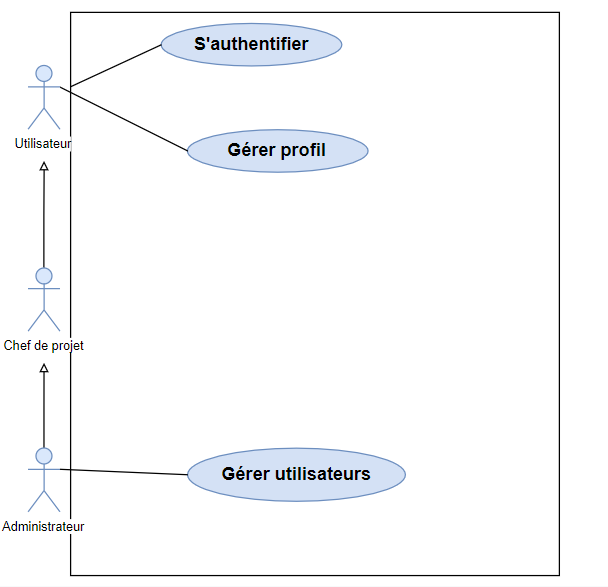
\includegraphics[scale=0.6]{Rsprint1.PNG}
	\caption{Diagramme de cas d'utilisation du sprint 1}
	\label{Diagramme de cas d'utilisation du sprint 1}
\end{figure} 
Comme le montre la figure 3.1, ce sprint permet aux utilisateur d'accéder facilement à l'application et de gérer leurs données personnelles sur leurs profils. Ainsi, pendant cette itération, l'administrateur devient capable de gérer tous les utilisateurs inscrits dans l'application.
\section{Gestion des comptes }

Cette partie est consacrée à la gestion des comptes personnels des utilisateurs. Ce dernier est composé  par les cas d'utilisation "s'authentifier" et "gérer profil". 
\subsection{Analyse}
Afin de mieux  détailler le fonctionnement et assimiler les cas d'utilisation de la première partie   constituant  ce sprint, nous allons établir, dans cette section,  leurs raffinements en livrant
une description sur les différents scénarios possibles.
\begin{itemize}
	\item \textbf{Raffinement du cas d'utilisation "S'authentifier"}\\
\end{itemize}

	\begin{figure}[H]
		\centering
		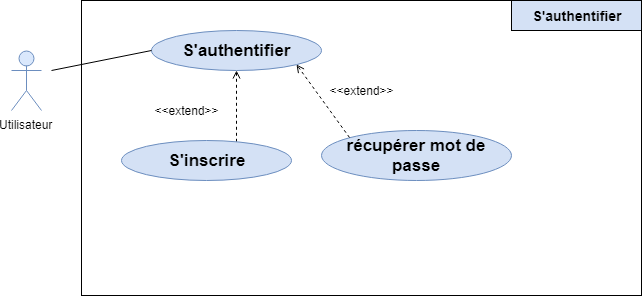
\includegraphics[scale=0.7]{Rauth.png}
		\caption{Raffinement du cas d'utilisation: S'authentifier}
		\label{Raffinement du cas d'utilisation: S'authentifier}
	\end{figure} 
Comme le montre la figure 3.2 un utilisateur peut soit s'authentifier ou bien créer un compte s'il s'agit d'un nouveau
utilisateur. L'application offre la possibilité de récupérer son mot de passe en cas d'oubli
en envoyant un nouveau mot de passe par émail.
Si l'utilisateur est authentifié avec succès, une page d'accueil sera ouverte, sinon, il sera
redirigé vers la page d'authentification.

 \textbf{Description textuelle du cas d'utilisation "Créer un compte"}

\begin{table}[H]
	\begin{tabular}{|l|l|}
		\hline
		\textbf{Acteur}                              & Utilisateur                                                                                                                                               \\ \hline
		\textbf{Description}                         & Ajouter un utilisateur au système.                                                                                                                        \\ \hline
		\textbf{Préconditions}                       & Disponibilité d'accès au serveur.                                                                                                                         \\ \hline
		\textbf{Post-conditions}                     & Utilisateur inscrit.                                                                                                                                      \\ \hline
		\multirow{4}{*}{\textbf{Scénario principal}} & \begin{tabular}[c]{@{}l@{}}1. L'utilisateur remplit le formulaire, valide reCAPTCHA\\ puis confirme.\end{tabular}                                         \\ \cline{2-2} 
		& 2. Le système  vérifie l'unicité de l'utilisateur.                                                                                                        \\ \cline{2-2} 
		& \begin{tabular}[c]{@{}l@{}}3. Le système génère un mot de passe aléatoire et l'envoie à \\ l'utilisateur par mail.\end{tabular}                           \\ \cline{2-2} 
		& 4.  Le système ajoute l'utilisateur .                                                                                                                     \\ \hline
		\textbf{Scénario altérnatif}                 & \begin{tabular}[c]{@{}l@{}}2.a Le système retourne un message d'erreur indiquant \\ l'existence d'un utilisateur avec des cordonnées pareil.\end{tabular} \\ \hline
	\end{tabular}

\caption{Description textuelle du << Créer un compte >> }
\label{Description textuelle du << Créer un compte >>}
\end{table}
\begin{itemize}
	\item  \textbf{Raffinement du cas d'utilisation "Gérer le profil"}
\end{itemize}
\begin{figure}[H]
	\centering
	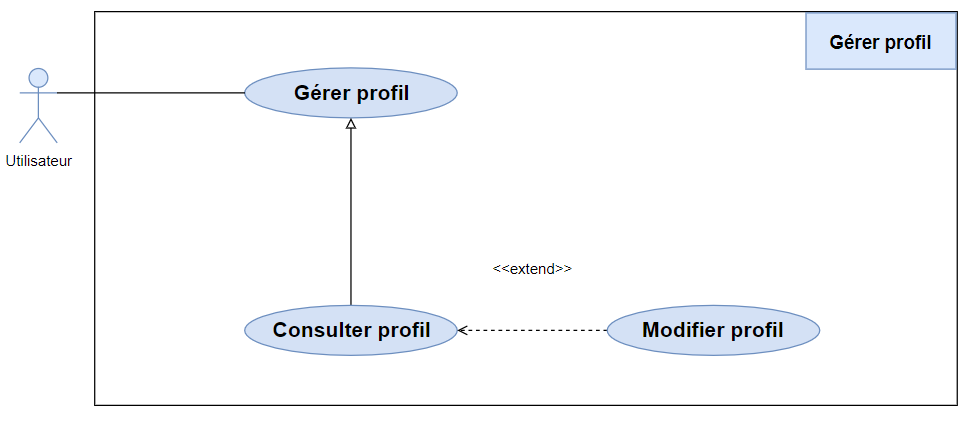
\includegraphics[ height=4cm, width=13cm]{Rprofil.PNG}
	\caption{Raffinement du cas d'utilisation:  Gérer le profil}
	\label{Raffinement du cas d'utilisation: Gérer le profil}
\end{figure} 

Le diagramme de cas d'utilisation de la figure 3.3  est une illustration des détails de la gestion du profil. En outre, ce diagramme montre la relation d'inclusion entre la consultation du profil et sa mise à jour.
\subsubsection{Description textuelle du sous cas d'utilisation: "Mettre à jour le profil"}

\begin{table}[ht]
	\begin{tabular}{|l|l|}
		\hline
		\textbf{Acteur}                               & Utilisateur.                                                                                                       \\ \hline
		\textbf{Description}                          & Mettre à jour profil.                                                                                              \\ \hline
		\textbf{Préconditions}                        & Utilisateur authentifié.                                                                                           \\ \hline
		\textbf{Post-conditions}                      & Profil mis à jour.                                                                                                 \\ \hline
		\multirow{5}{*}{\textbf{Scénario principal}}  & \begin{tabular}[c]{@{}l@{}}1. L'utilisateur clique sur  l'icône de mise à jour du profil.\end{tabular}           \\ \cline{2-2} 
		& 2. Le système afficher un formulaire.                                                                              \\ \cline{2-2} 
		& 3. L'utilisateur remplie le formulaire.                                                                            \\ \cline{2-2} 
		& 4. Le système met à jour le profil.                                                                                \\ \cline{2-2} 
		& 5.  Le système affiche le profil modifié.                                                                          \\ \hline
		\multirow{2}{*}{\textbf{Scénario altérnatif}} & \begin{tabular}[c]{@{}l@{}}3.a L'utilisateur laisse un champ vide, ou saisit de données\\ invalides.\end{tabular} \\ \cline{2-2} 
		& \begin{tabular}[c]{@{}l@{}}3.b Le système répond avec des messages d'erreurs.\end{tabular}                      \\ \hline
	\end{tabular}

\caption{Description textuelle du << Mettre à jour  le profil  >> }
\label{Description textuelle du << Mettre à jour le profil >>}
\end{table}


\subsection{Conception} 
Les diagrammes de séquence objet permettent de représenter les vues dynamiques du système en montrant les
collaborations entre les objets selon un point de vue temporel. Dans ce qui suit, nous allons
représenter les diagrammes de séquences les plus importants de la première partie de cette itération.\\
\textbf{Diagramme de séquences  du cas d'utilisation  "S'authentifier"}\\
\begin{figure}[H]
	\centering
	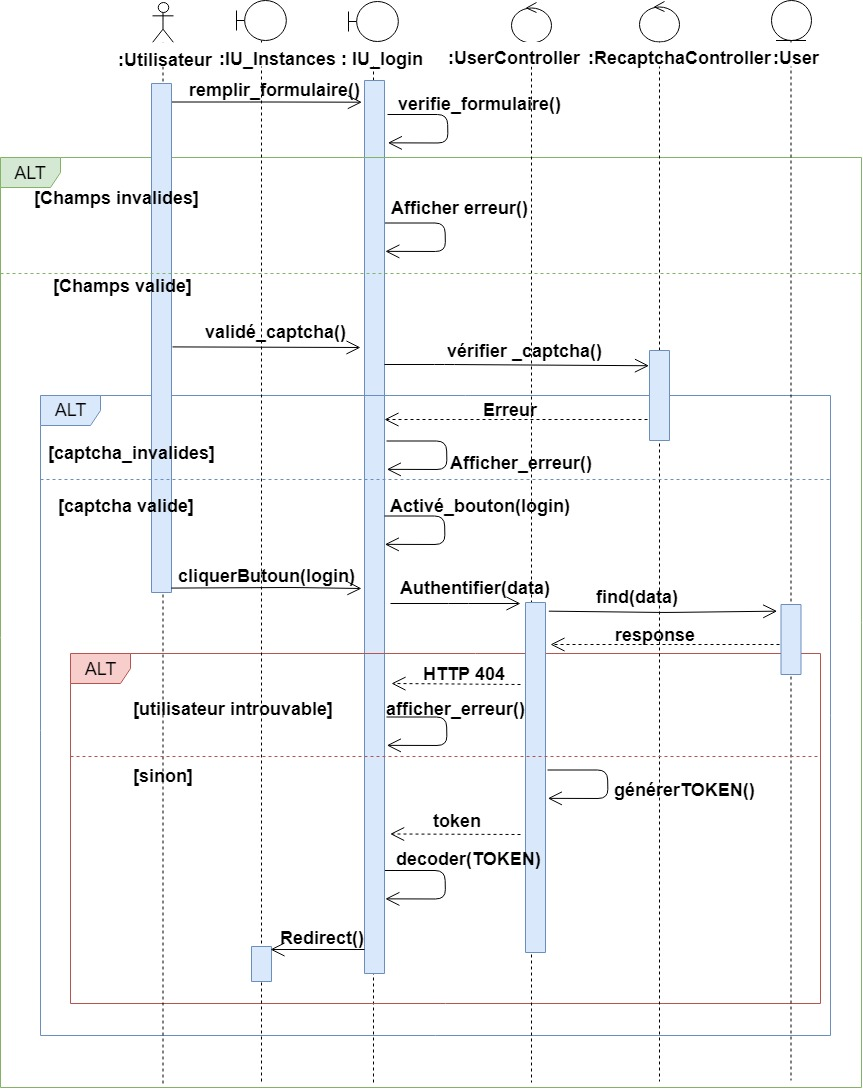
\includegraphics[scale=0.5]{login1.jpg}
	\caption{Diagramme de séquence: S'authentifier}
	\label{Diagramme de séquence: S'authentifier}
\end{figure} 

La figure 3.4  présentée ci dessous décrit la  procédure d'authentification à l'application. Tout d'abord,  l'utilisateur saisit son email et mot de passe. Une validation des champs se produit automatiquement, s'ils sont  invalides, un message d'erreur s'affiche, sinon  l'utilisateur continue sa procédure en validant recaptcha. Une fois validé et le bouton de connexion est appuyé,  les données s'envoient au contrôleur pour vérifier l'existence et la correspondance des coordonnées. Si c'est le cas, le contrôleur génère un token et l'émet pour qu'il soit décodé et utilisé dans l'envoie des prochaines requêtes, sinon il retourne une requête http portant le statut 401 indiquant la non autorisation d'accès.


\textbf{Diagramme de séquence du sous cas d'utilisation "Réinitialiser mot de passe"}\\
\begin{figure}[H]
	\centering
	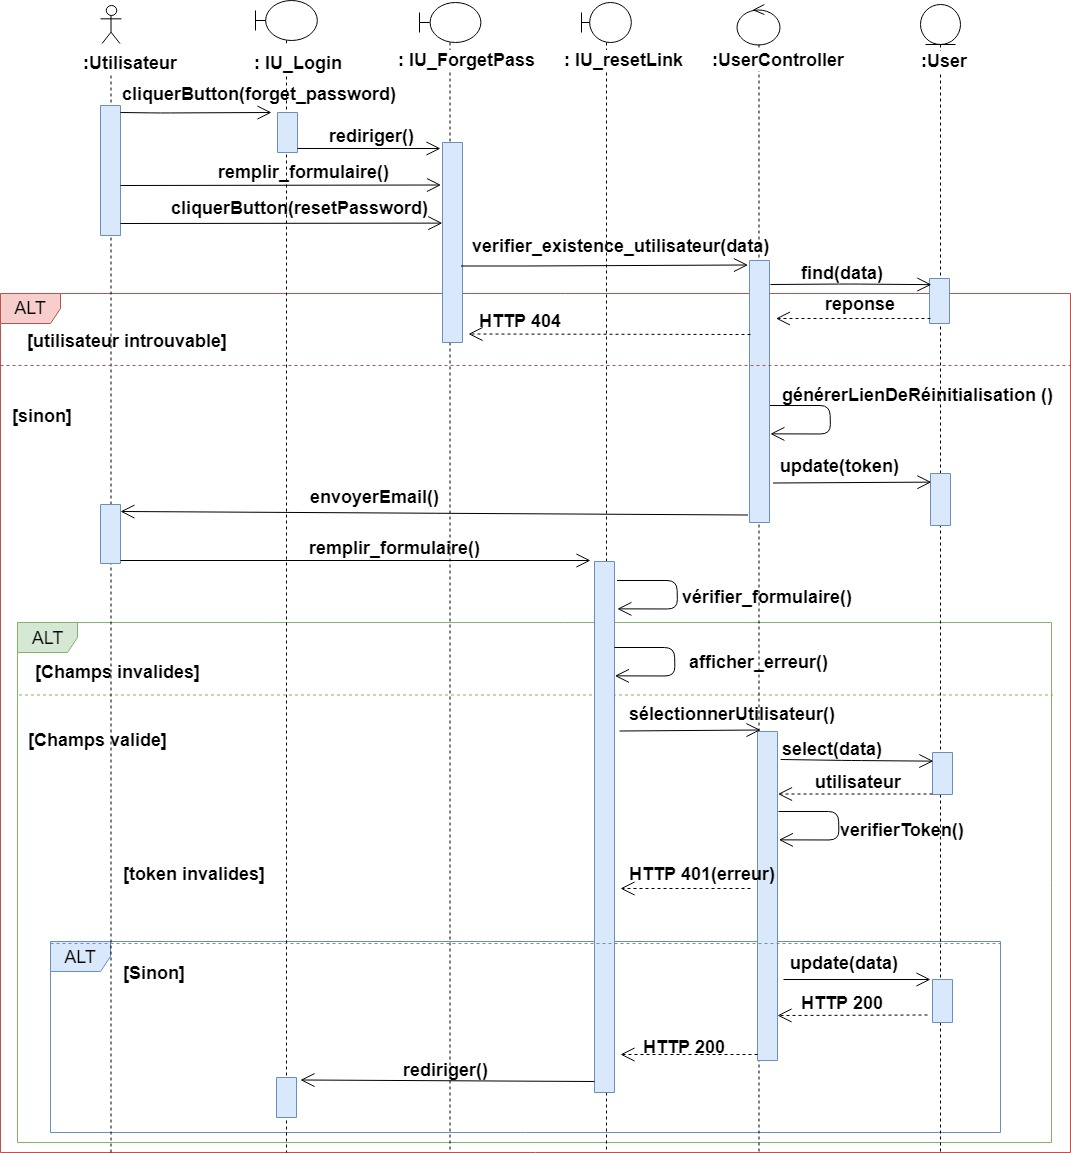
\includegraphics[scale=0.4]{resetpassword.jpg}
	\caption{Diagramme de séquence: Réinitialiser mot de passe}
	\label{Diagramme de séquence: Réinitialiser mot de passe}
\end{figure}

Le diagramme de la figure 3.5 ci dessus, met en évidence la procédure de  réinitialisation du mot de passe. Tout d'abord, l'utilisateur demande un nouveau mot de passe en appuyant sur le bouton correspondant. Ensuite, il sera redirigé vers l'interface de réinitialisation du mot de passe, là ou il devra saisir son email. Une fois son existence est validée, le contrôleur régénère un token et envoie un email contenant un lien de régénération du mot de passe.
L'utilisateur choisit alors un nouveau mot de passe et l'émet au contrôleur pour mettre à jour l'ancien token et l'ancien mot  de passe. Le contrôleur répond avec une requête HTTP de statut 200 si tout est bien. 

\subsubsection{Diagramme de séquence du cas d'utilisation: "Mettre à jour son profil"}

\begin{figure}[H]
	\centering
	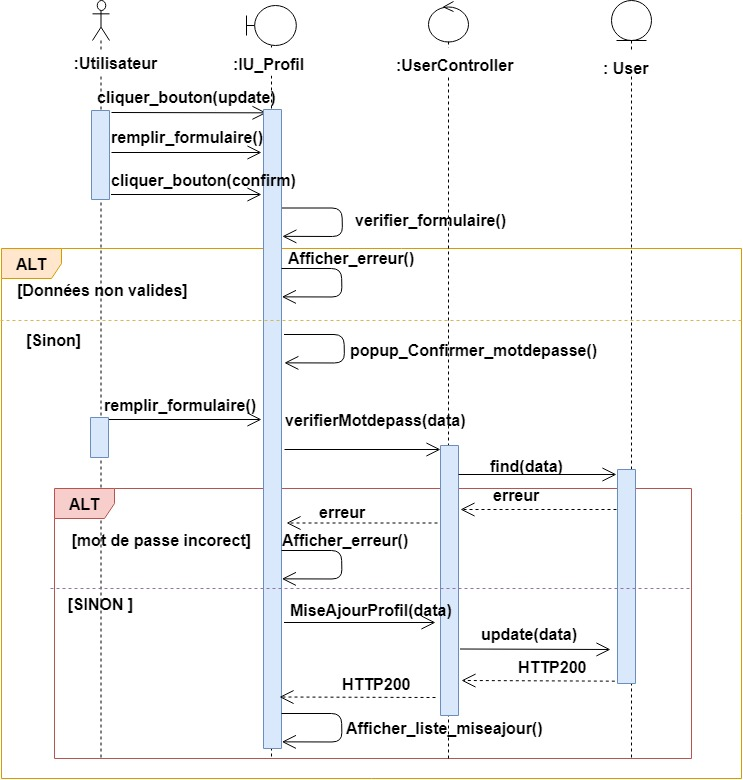
\includegraphics[height=11cm,width=14cm]{Majprofil-Page-1.jpg} 
	\caption{Diagramme de séquence: Mettre à jour profil}
	\label{Diagramme de séquence: Mettre à jour profil}
\end{figure}
Le diagramme de la figure 3.6 décrit la procédure de modification des données personnelles. En effet, l'utilisateur accède à son profil, là ou il clique sur l'icône d'activation de mode édition. Il saisit les données à modifier et  confirme sa modification en cliquant sur le bouton confirme. Une fois cliqué, une modale s'ouvre demandant de confirmer encore par le saisie du mot de passe. 
L'utilisateur saisit alors son mot de passe. Ce dernier est envoyé au contrôleur pour valider son existence. S'il est valide  les changements seront pris en compte et le contrôleur retourne une requête http de statut 200 sinon il retourne une requête de statut 401.

\section{Gestion des utilisateurs}
Cette partie est consacrée à la gestion des utilisateurs. Elle est composée  par le cas d'utilisation "gérer les utilisateurs". 
\subsection{Analyse}
Dans ce qui suit, nous allons offrir une vue d'ensemble des différentes fonctionnalités relatives à la deuxième partie de ce sprint. Ensuite, nous allons raffiner et décrire
les cas d'utilisation les plus prioritaires.
\subsubsection{Raffinement du cas d'utilisation: "Gérer utilisateurs" }
\begin{figure}[H]
	\centering
	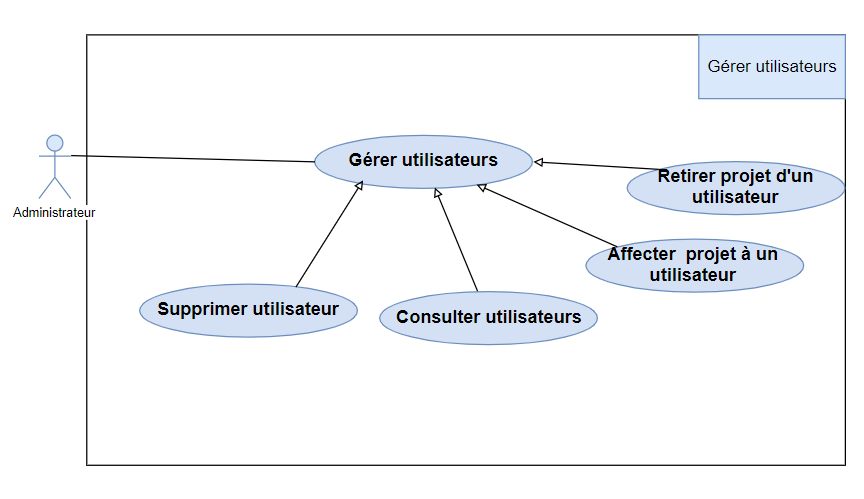
\includegraphics[ height=4.8cm, width=14cm]{Rgererusers.PNG}
	\caption{Raffinement du cas d'utilisation: Gérer les utilisateurs}
	\label{Raffinement du cas d'utilisation: Gérer les utilisateurs}
\end{figure}
Le diagramme de la figure 3.7 présente un raffinement relatif au cas d'utilisation "gérer les utilisateurs". En effet, à travers la consultation de la liste des utilisateurs nous pouvons  soit supprimer, soit affecter un projet à un utilisateur ou bien retirer un projet de l' utilisateur.
\subsubsection{Description textuelle du sous cas d'utilisation: "Supprimer un utilisateur"}

% Please add the following required packages to your document preamble:
% \usepackage{multirow}
\begin{table}[H]
	\begin{tabular}{|l|l|}
		\hline
		\textbf{Acteur}                               & Administrateur.                                                                                                                                             \\ \hline
		\textbf{Description}                          & Supprimer un compte utilisateur du système.                                                                                                                 \\ \hline
		\textbf{Préconditions}                        & Administrateur authentifié.                                                                                                                                 \\ \hline
		\textbf{Post-conditions}                      & Utilisateur supprimé.                                                                                                                                       \\ \hline
		\multirow{5}{*}{\textbf{Scénario principal}}  & \begin{tabular}[c]{@{}l@{}}1. L'administrateur clique sur l'icône de \\ suppression.\end{tabular}                                                           \\ \cline{2-2} 
		& 2. . Le système affiche une modale de confirmation.                                                                                                         \\ \cline{2-2} 
		& 3. L'administrateur clique sur confirme son choix.                                                                                                          \\ \cline{2-2} 
		& \begin{tabular}[c]{@{}l@{}}4. Le système supprime l'utilisateur correspondant et affiche \\ un message manifestant la réussite de l'opération.\end{tabular} \\ \cline{2-2} 
		& 5. Le système affiche la nouvelle liste des utilisateurs.                                                                                                   \\ \hline
		\multirow{2}{*}{\textbf{Scénario altérnatif}} & \begin{tabular}[c]{@{}l@{}}2.a L'administrateur décide d'annuler l'opération de \\ suppression.\end{tabular}                                                \\ \cline{2-2} 
		& \begin{tabular}[c]{@{}l@{}}2.b Le système ferme la modale et affiche la liste des\\ utilisateurs mise à jour.\end{tabular}                                  \\ \hline
	\end{tabular}

\caption{Description textuelle du << Supprimer un utilisateur >> }
\label{Description textuelle du << Supprimer un utilisateur >>}
\end{table}
% Il faut ajouter que il peut chercher un utilisateur inexistant
\subsection{Conception}
Afin de décortiquer et détailler les cas d'utilisation précédemment cités, nous présentons dans ce qui suit les diagrammes de séquences des cas d'utilisation les plus importants
\subsubsection{Diagramme de séquence du cas d'utilisation: "Supprimer un utilisateur"}

\begin{figure}[H]
	\centering
	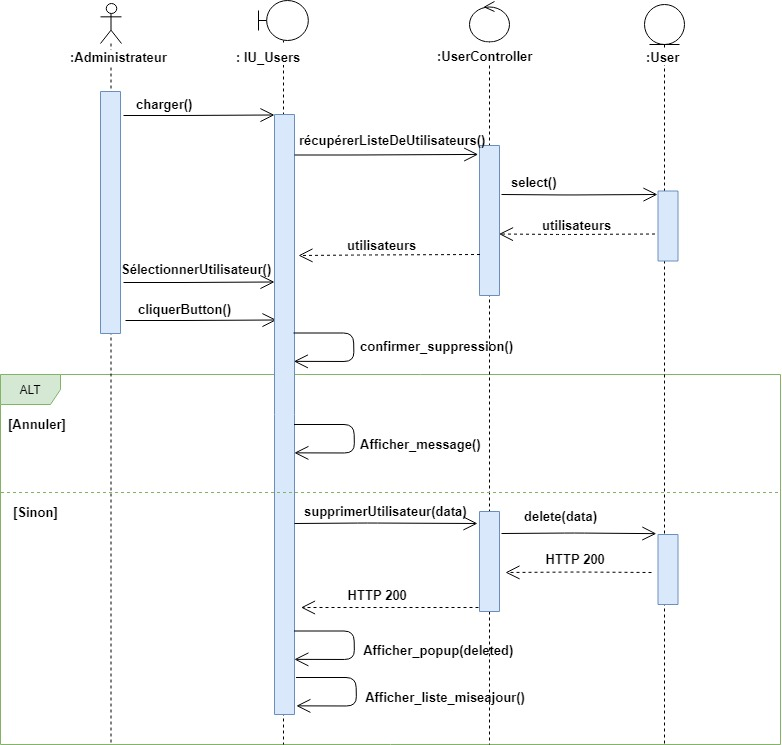
\includegraphics[scale=0.55]{deleteuser.jpg}
	\caption{Diagramme de séquence: Supprimer un utilisateur}
	\label{Diagramme de séquence: Supprimer un utilisateur}
\end{figure}
Le diagramme de la figure 3.8 décrit l'opération de suppression d'un utilisateur. Tout d'abord, l'administrateur accède à la liste des utilisateurs. Ensuite, 
Il clique sur le bouton de suppression correspondant. Une fois cliqué, une modale de confirmation s'ouvre. Là ou il peut soit annuler l'opération, soit la confirmer. S'il appuie sur le bouton de confirmation  les données nécessaires à la suppression seront émises au contrôleur pour 
vérifier l'existence de l'utilisateur à partir de son email. Par la suite, le contrôleur retourne une requête http de statut 200, dans le cas ou l'utilisateur existe. Il retourne une erreur, dans le cas contraire.


\section{Réalisation}
\subsection{Sécurité}
\begin{itemize}
	\item \textbf{Authentification avec reCAPTCHA}: Permettant de vérifier l'identité annoncée, s'assurer de la non usurpation d'identité de la personne en question, empêcher les accès  automatisés par les robots et   toute tentative de spam.
	\item \textbf{Autorisation}: Permettant la vérification de privilèges de chaque utilisateur pour accéder à la ressource demandée.Dans Symfony 4, il s'agit d'un fichier de configuration  "Security.yaml"  réparti en sections dont chaque section assure un role bien important dans la sécurité 
	\begin{itemize}
		\item Section "firewalls" met en évidence la méthode d'authentification elle peut être soit par login et mot de passe, soit par la méthode HTTP ou bien à travers un compte de réseau social.
		\item Section "access control"  permet de gérer les droits d'accès des utilisateurs.
		\item Section "encoders" permet de spécifier l'algorithme de hashage  à utiliser pour stocker le mot de passe.
	\end{itemize} 
\item \textbf{Cryptage des mots de passe}: 
Pour se protéger contre les attaques et assurer la confidentialité et  l'intégrité des mots de passe des utilisateurs, nous avons opté pour le chiffrement de ses derniers par  l'algorithme "argon2i" à travers la section "encoders" de fichier "Security.yaml" de Symfony.
\item \textbf{Sécurisation des APIs}: L'échange des informations concernant l'utilisateur couramment authentifié est sécurisé au moyen des jetons JWT pour (Json Web Token) généré par le serveur.

 \textbf{Structure de JWT} \\Ce standard de transmission des informations est composé de trois parties définies par la figure 3.5. 



	\begin{itemize}
	\item Header: contient le type de jeton et l'algorithme utilisé pour la signature.
	\item Payload: contient toutes les données personnelles de l'utilisateur.
	\item Signature:  hachage d'en-tête, de charge utile de la partie Payload et d'une clé secrète codée.
	 	
\end{itemize}
	\begin{figure}[H]
	\centering
	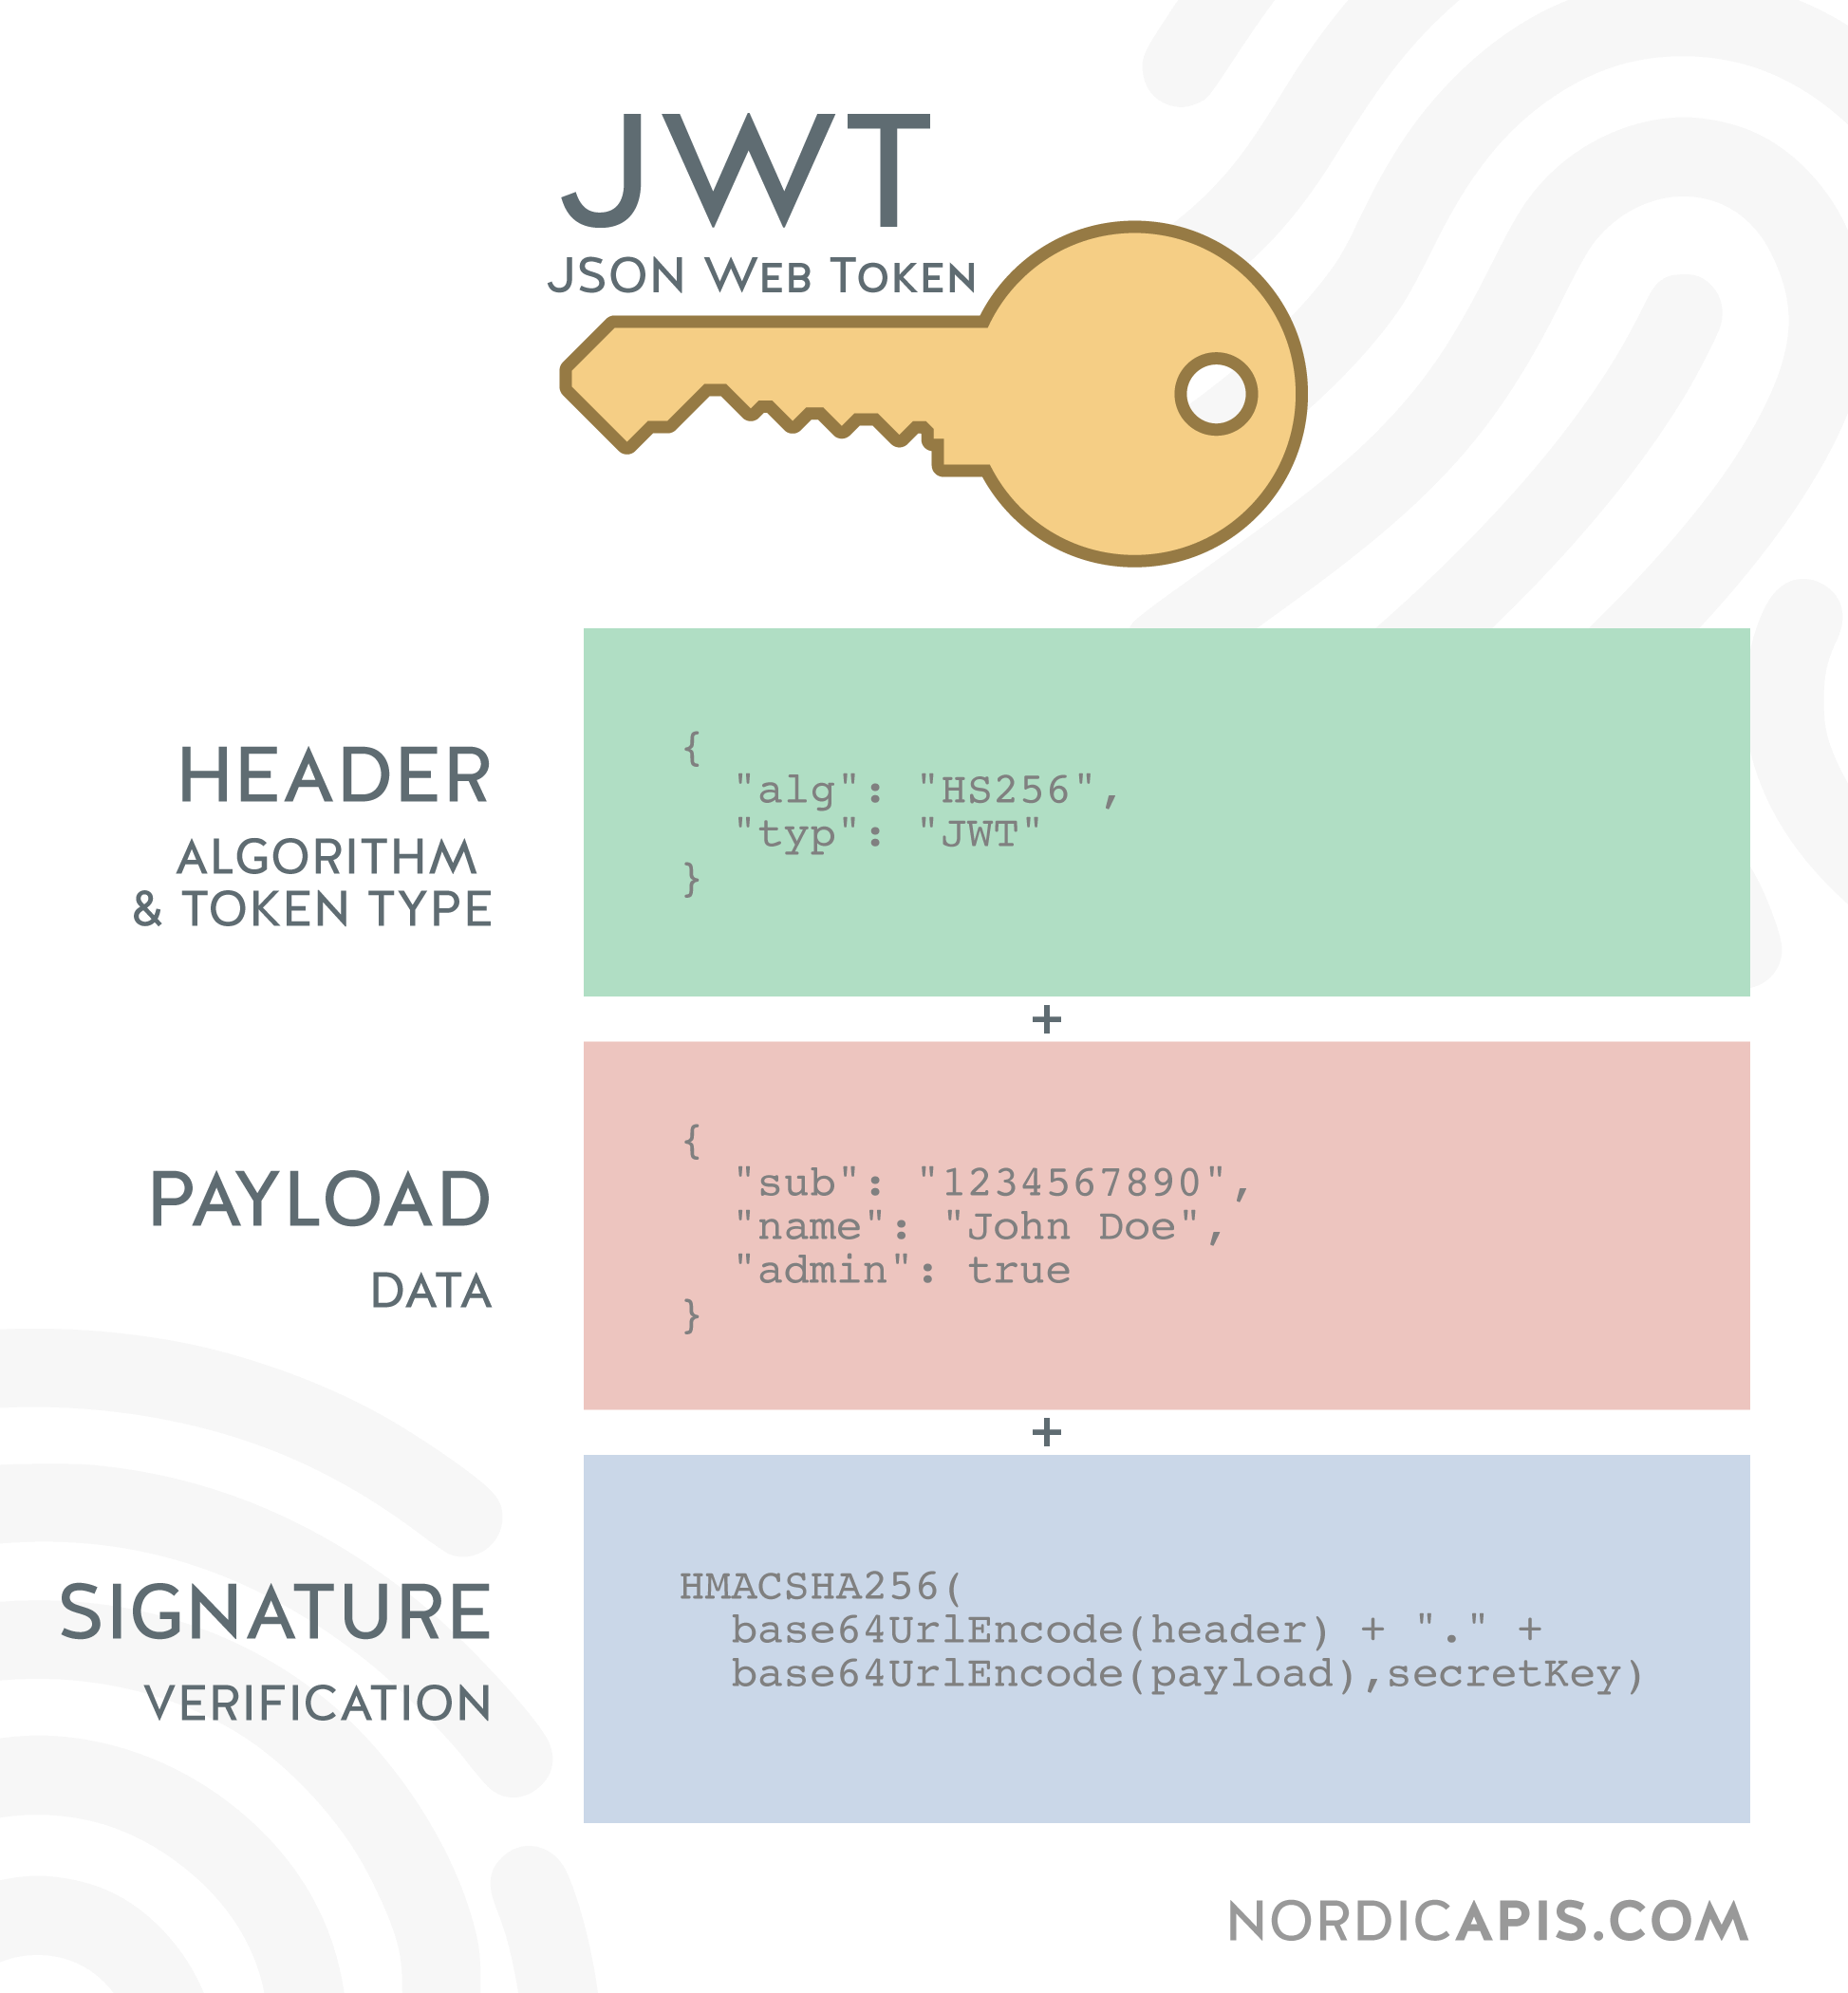
\includegraphics[scale=0.09]{jwt2.png}
	\caption{Structure de JWT}
	\label{Structure de JWT}
\end{figure} 
\newpage
\textbf{Fonctionnement de JWT}
	\begin{figure}[H]
	\centering
	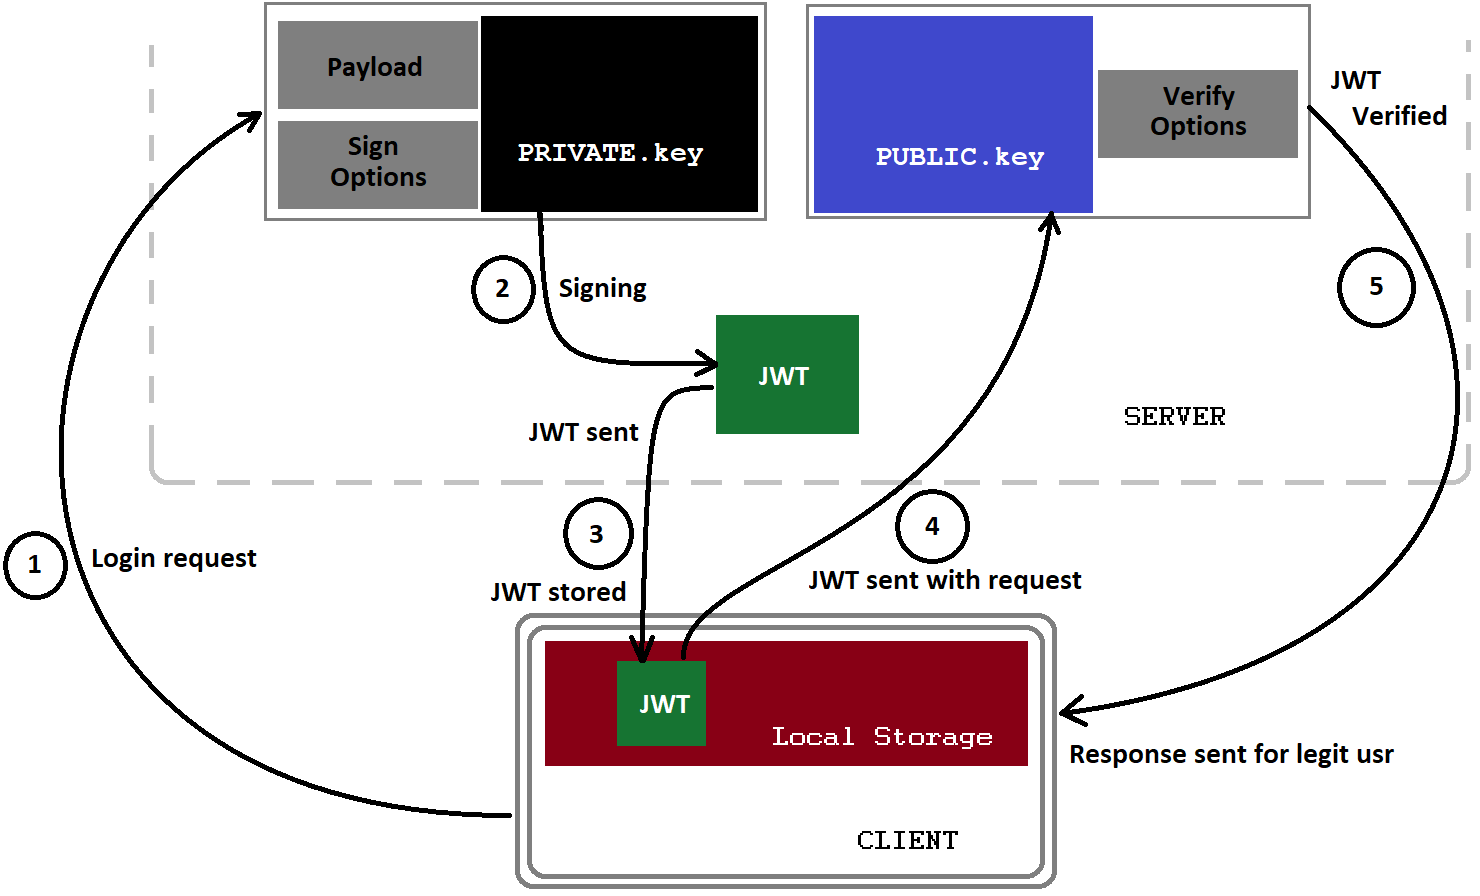
\includegraphics[scale=0.2]{jwt.png}
	\caption{Fonctionnement de JWT}
	\label{Fonctionnement de JWT}
\end{figure} 

Comme présenté par la figure 3.10 lorsqu'un utilisateur envoie une requête avec les paramètres requis tels que le mail d'utilisateur et
son mot de passe. L'application vérifie si le mail d'utilisateur et le mot de passe sont valides. Lors de
la validation, l'application créera un jeton à l'aide d'un payload et d'une clé secrète. Il renverra
ensuite le jeton à l'utilisateur pour l'enregistrer à "local storage" et l'envoyer à chaque demande. Lorsque l'utilisateur
envoie une requête avec ce jeton, l'application vérifie la validité avec la même clé secrète. Si le
jeton est valide, la demande est envoyée, sinon l'application enverra un message d'erreur approprié.



\end{itemize}
\subsection{Interfaces}
Nous montrons le résultat du sprint courant,dans la partie qui suit, à travers des imprimes écran.
\begin{figure}[!htb]
	\minipage{0.4\textwidth}
	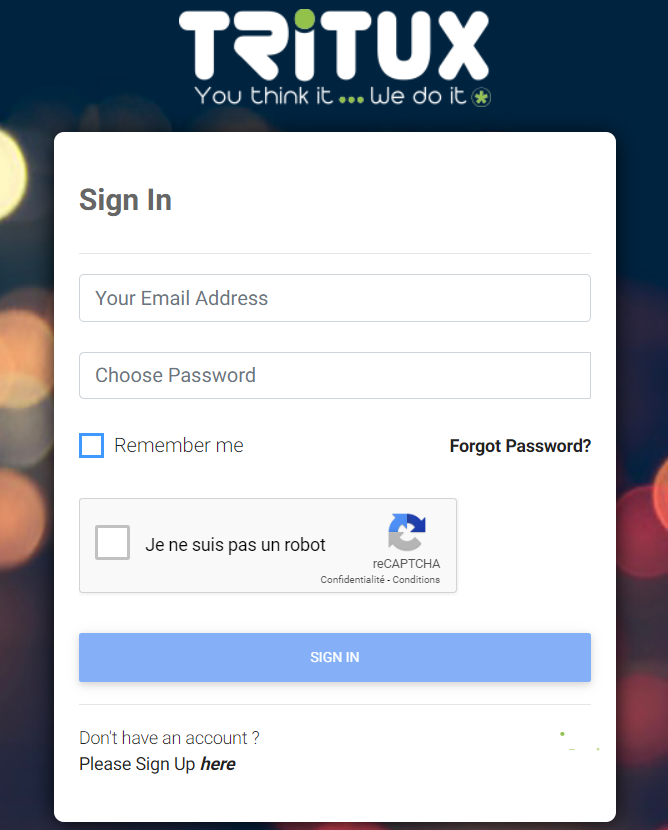
\includegraphics[width=\linewidth, height=7.3cm]{login.PNG}
	\caption{Interface de connexion à l'application }\label{fig:Interface de connexion à l'application }
	\endminipage\hfill
	\minipage{0.4\textwidth}
	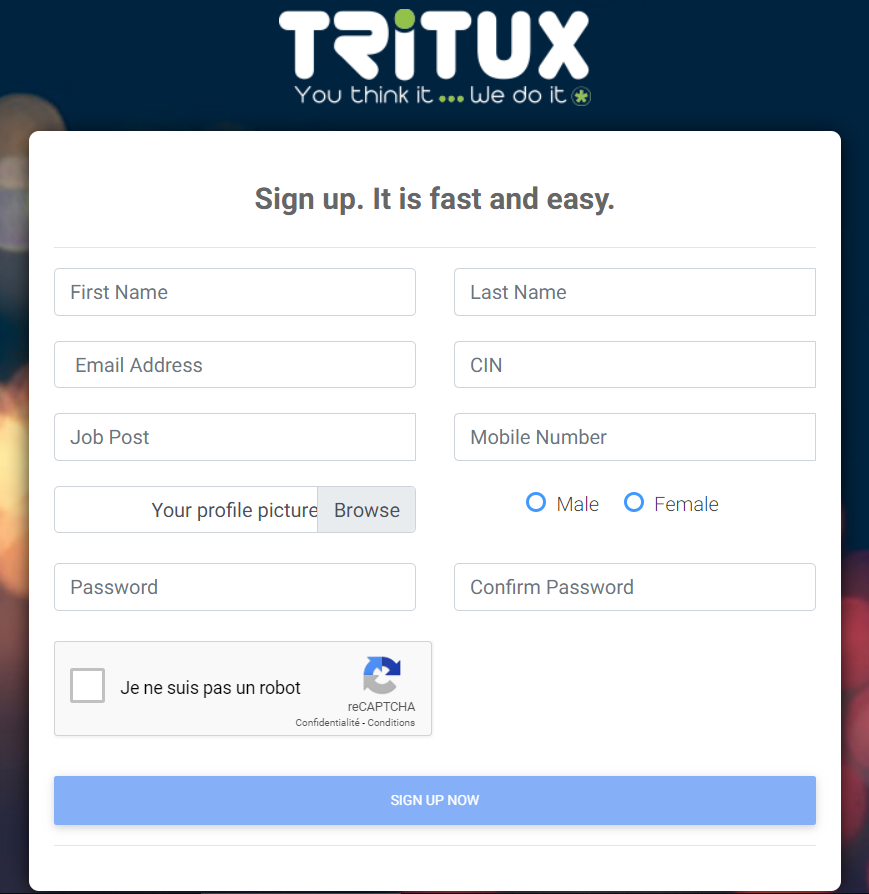
\includegraphics[width=\linewidth,height=7.5cm]{inscription.PNG}
	\caption{Interface d'inscription}\label{fig:Interface d'inscription }
	\endminipage\hfill
\end{figure}

La figure 3.11 montre l'interface de l'ouverture de l'application. Si un utilisateur ne possède pas de compte il peut s'inscrire à travers la figure 3.12  ou  bien s'il est déjà inscrit mais il a oublié son mot de passe, il peut le réinitialiser à travers les interfaces décrites dans les figures 3.13 et 3.14.

\begin{figure}[!htb]
	\minipage{0.4\textwidth}
	
\includegraphics[width=\linewidth, height=7.4cm]{reinitmdp.PNG}
	\caption{Interface de réinitialisation du mot de passe }\label{fig: Interface de réinitialisation du mot de passe }
	\endminipage\hfill
	\minipage{0.4\textwidth}
	
\includegraphics[width=\linewidth, height=7cm]{recoverpass1.PNG}
	\caption{Interface d'affectation d'un nouveau mot de passe en cas d'oubli}\label{fig:Interface d'affectation d'un nouveau mot de passe en cas d'oubli}
	\endminipage\hfill
\end{figure}

\begin{figure}[H]
\centering
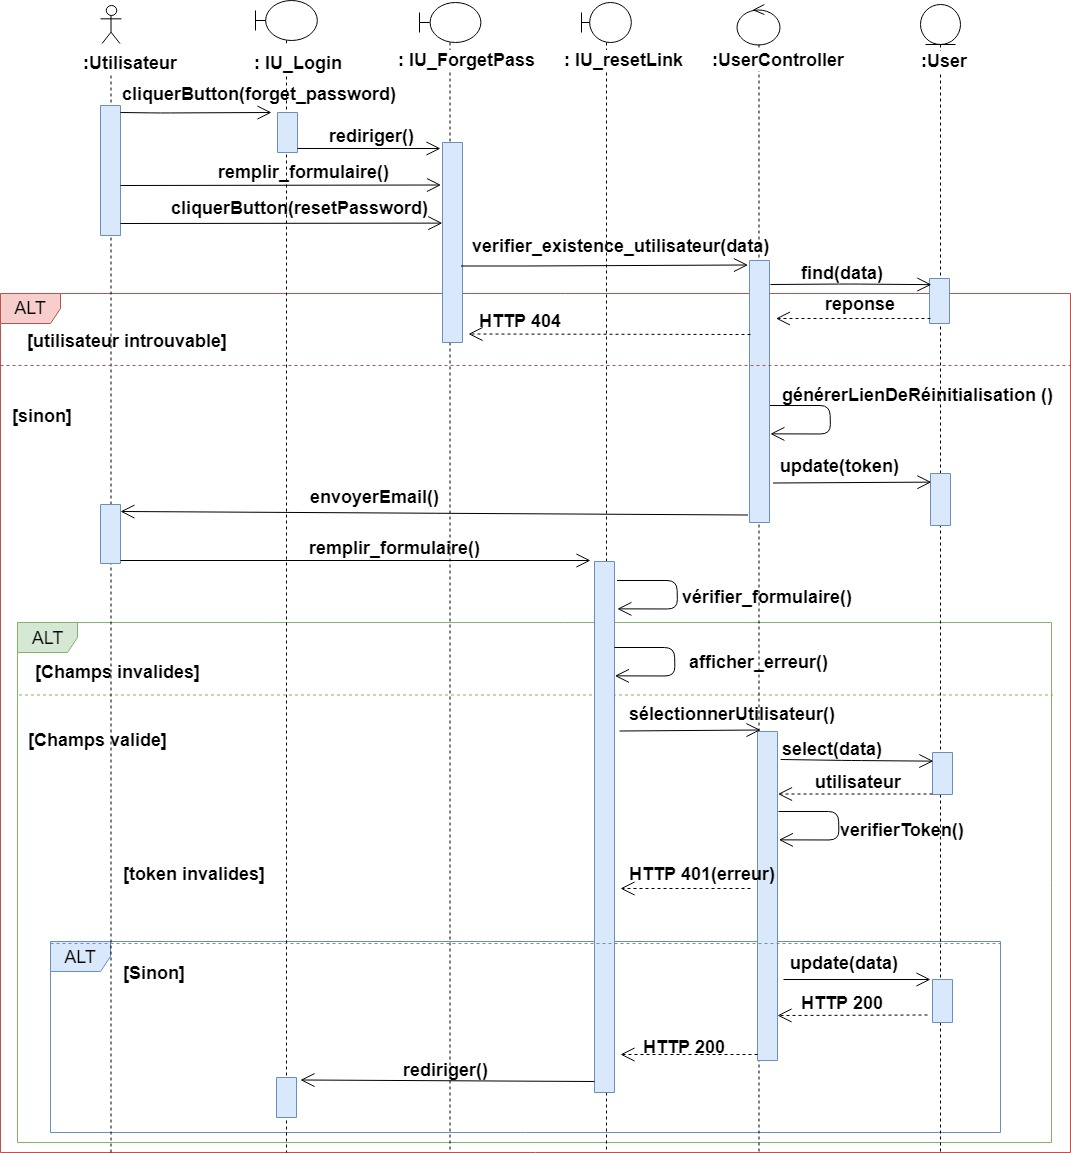
\includegraphics[height=10cm,width=15cm]{resetpassword.jpg}
\caption{ Email de réinitialisation du mot de passe }
\label{Email de réinitialisation du mot de passe}
\end{figure}
La figure 3.15 représente l'interface de gestion du profil. Dedans l'utilisateur aura la possibilité de modifier ses données personnelles comme le montre la figure 3.16.


	\begin{figure}[H]
	\centering
	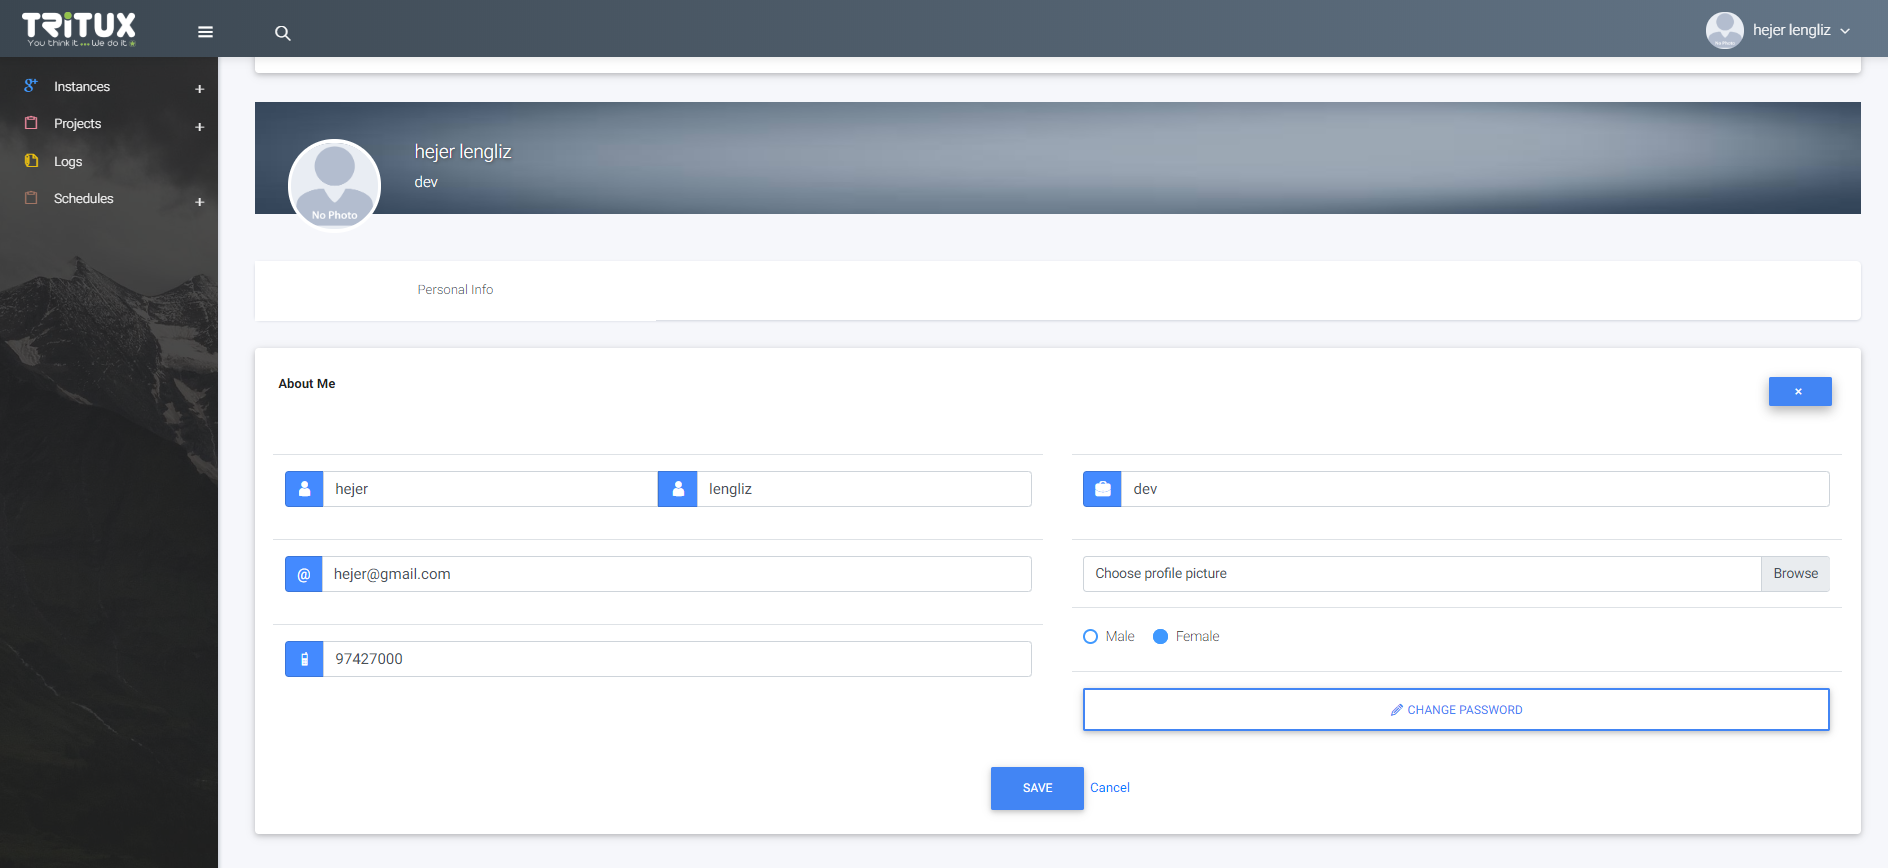
\includegraphics[scale=0.35]{editprofile.PNG}
	\caption{Interface de mise à jour du profil}
	\label{Interface de mise à jour du profil}
\end{figure}
	\begin{figure}[H]
	\centering
	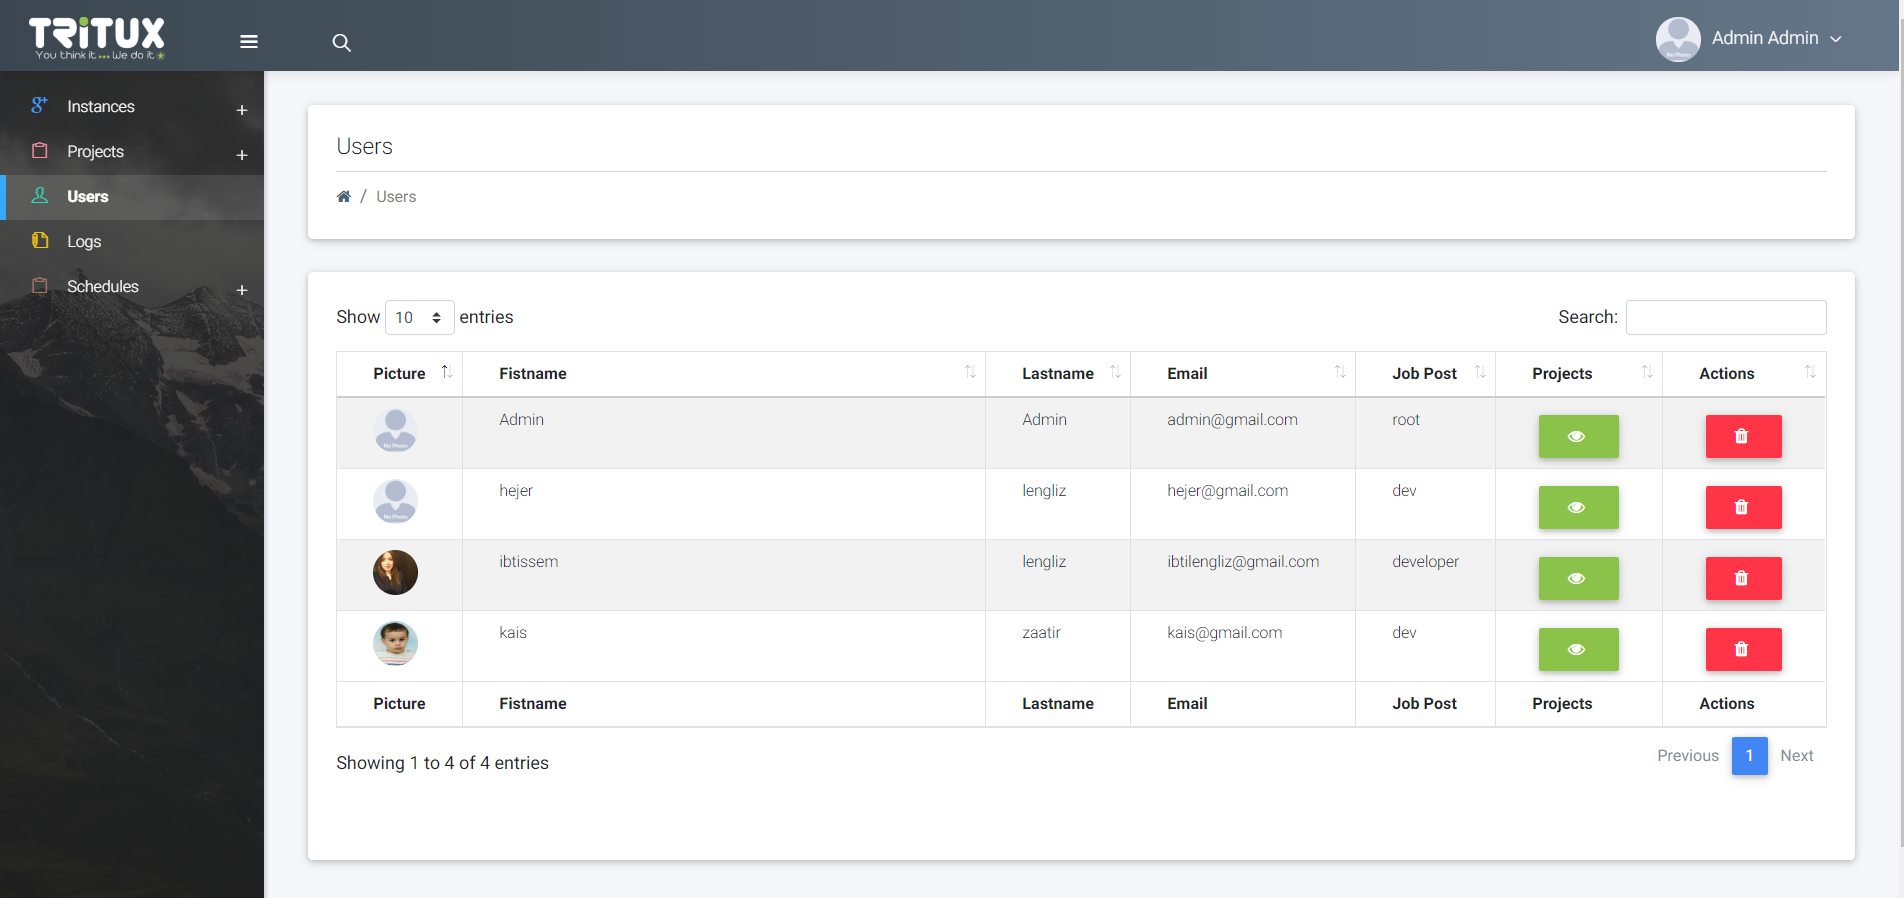
\includegraphics[scale=0.35]{users.PNG}
	\caption{Interface de gestion des utilisateurs}
	\label{Interface de gestion des utilisateurs}
\end{figure}
La figure 3.16 représente l'interface de gestion des utilisateurs, grâce à laquelle l'administrateur
pourra rechercher , supprimer un utilisateur et  affecter ou retirer un projet de l'utilisateur.


\section{Conclusion}
Le résultat d'un sprint est un produit livrable au client. Tout au long de ce chapitre,
nous avons réussi à produire un incrément ayant suffisamment de valeur pour le client
et pourra être utilisé dans un environnement de production. Dans le chapitre qui suit,
notre effort sera consacré pour produire une nouvelle valeur métier couvrant les fonctionnalités
de management des projets et des machines virtuelles.


\chapter{Sprint2: Management des projets et des VMs}
\section {Introduction}
L'objectif de ce chapitre est de présenter la seconde itération du cycle de vie de notre
projet. Nous allons entamer par identifier les tâches à réaliser dans le Backlog du Sprint pour
passer par la suite aux phases d'analyse et de conception. Nous finirons par exposer la phase de
réalisation de ce module.\\
Nous avons découpés ce sprint en deux parties, une pour la gestion des projets et une autre pour le management des instances de VM qui est un élément majeur de notre application.

\section{Etude fonctionnelle}
\subsection{Backlog du Sprint} 
Le Backlog du sprint dévoilé par le tableau 3.1 comprend une liste des travaux, de chaque user story, qui seront faites durant ce sprint.



\begin{table}[H]
	\begin{tabular}{|l|l|l|l|}
		\hline
		\textbf{ID}          & \textbf{User Story}                                                                                                                                                     & \textbf{Description}                                                                                                                                                     & \textbf{Esti.} \\ \hline
		\multirow{3}{*}{3.1} & \multirow{3}{*}{\begin{tabular}[c]{@{}l@{}}En tant que Team leader, je souhaite\\ consulter mes projets.\end{tabular}}                                                  & \begin{tabular}[c]{@{}l@{}}Créer la "datatable" \\ de sélection de tous \\ les projets.\end{tabular}                                                                     & 3              \\ \cline{3-4} 
		&                                                                                                                                                                         & \begin{tabular}[c]{@{}l@{}}Implémenter l'API de\\  sélection des utilisateurs.\end{tabular}                                                                              & 3              \\ \cline{3-4} 
		&                                                                                                                                                                         & Consommer l'API.                                                                                                                                                         & 3              \\ \hline
		\multirow{3}{*}{3.2} & \multirow{3}{*}{\begin{tabular}[c]{@{}l@{}}En tant que administrateur, je souhaite\\ \\ supprimer un projet.\end{tabular}}                                              & \begin{tabular}[c]{@{}l@{}}Créer la modale de \\ confirmation de\\ suppression\end{tabular}                                                                              & 2              \\ \cline{3-4} 
		&                                                                                                                                                                         & \begin{tabular}[c]{@{}l@{}}Implémenter l'API de\\  suppression d'un \\  utilisateur.\end{tabular}                                                                        & 3              \\ \cline{3-4} 
		&                                                                                                                                                                         & Consommer l'API.                                                                                                                                                         & 3              \\ \hline

\end{tabular}
\end{table}
% Please add the following required packages to your document preamble:
% \usepackage{multirow}
\begin{table}[H]
	\begin{tabular}{|l|l|l|l|}
		\hline
		\textbf{ID}          & \textbf{User Story}                                                                                                                                                     & \textbf{Description}                                                                                                                                                     & \textbf{Esti.} \\ \hline
		\multirow{3}{*}{3.3} & \multirow{3}{*}{\begin{tabular}[c]{@{}l@{}}En tant que administrateur, je souhaite \\ créer un projet.\end{tabular}}                                                    & \begin{tabular}[c]{@{}l@{}}Créer la vue de création\\  d'un projet.\end{tabular}                                                                                         & 2              \\ \cline{3-4} 
		&                                                                                                                                                                         & \begin{tabular}[c]{@{}l@{}}Générer l'API de création\\  d'un projet.\end{tabular}                                                                                        & 3              \\ \cline{3-4} 
		&                                                                                                                                                                         & Consommer l'API.                                                                                                                                                         & 3              \\ \hline
		\multirow{3}{*}{3.4} & \multirow{3}{*}{\begin{tabular}[c]{@{}l@{}}En tant que administrateur, je souhaite\\ modifier un projet.\end{tabular}}                                                  & \begin{tabular}[c]{@{}l@{}}Créer la modale de\\  modification d'un projet.\end{tabular}                                                                                  & 2              \\ \cline{3-4} 
		&                                                                                                                                                                         & \begin{tabular}[c]{@{}l@{}}Créer l'API de modification \\ d'un projet.\end{tabular}                                                                                      & 3              \\ \cline{3-4} 
		&                                                                                                                                                                         & Consommer l'API.                                                                                                                                                         & 3              \\ \hline
		\multirow{3}{*}{3.5} & \multirow{3}{*}{\begin{tabular}[c]{@{}l@{}}En tant que Team leader, je souhaite \\ ajouter un membre à mon projet.\end{tabular}}                                        & \begin{tabular}[c]{@{}l@{}}Créer la modale de\\  consultation, affectation et \\ de détachement d'un \\ membre du projet.\end{tabular}                                   & 2              \\ \cline{3-4} 
		&                                                                                                                                                                         & \begin{tabular}[c]{@{}l@{}}Créer l'API d'ajout \\ d'un membre à un projet.\end{tabular}                                                                                  & 3              \\ \cline{3-4} 
		&                                                                                                                                                                         & Consommer l'API.                                                                                                                                                         & 3              \\ \hline
		\multirow{2}{*}{3.6} & \multirow{2}{*}{\begin{tabular}[c]{@{}l@{}}En tant que Team leader, je souhaite \\ retirer un membre de mon projet.\end{tabular}}                                       & \begin{tabular}[c]{@{}l@{}}Créer l'API de retrait \\ d'un membre d'un projet.\end{tabular}                                                                               & 3              \\ \cline{3-4} 
		&                                                                                                                                                                         & Consommer l'API.                                                                                                                                                         & 3              \\ \hline
		\multirow{5}{*}{4.1} & \multirow{5}{*}{\begin{tabular}[c]{@{}l@{}}En tant que utilisateur je souhaite \\ consulter la liste des VMs.\end{tabular}}                                             & \begin{tabular}[c]{@{}l@{}}Spécifier le nom de \\ domaine de  l'application \\ auprès de Google Cloud\\   plateform.\end{tabular}                                        & 1              \\ \cline{3-4} 
		&                                                                                                                                                                         & \begin{tabular}[c]{@{}l@{}}Générer les clés nécessaires \\ pour  autoriser les requetes \\ auprès de Google Cloud\\  plateform.\end{tabular}                             & 1              \\ \cline{3-4} 
		&                                                                                                                                                                         & \begin{tabular}[c]{@{}l@{}}Créer la "datatable" de \\ sélection de toutes\\  les instances de VMs.\end{tabular}                                                          & 3              \\ \cline{3-4} 
		&                                                                                                                                                                         & \begin{tabular}[c]{@{}l@{}}Générer l'API de sélection \\ des VMs.\end{tabular}                                                                                           & 4              \\ \cline{3-4} 
		&                                                                                                                                                                         & Consommer l'API.                                                                                                                                                         & 3              \\ \hline
			\multirow{2}{*}{4.2} & \multirow{2}{*}{\begin{tabular}[c]{@{}l@{}}En tant que utilisateur je souhaite \\ orchestrer le fonctionnement des VMs.\end{tabular}}                                   & \begin{tabular}[c]{@{}l@{}}Générer l'API \\ d'orchestration de \\ fonctionnement des VMs.\end{tabular}                                                                   & 5              \\ \cline{3-4} 
		&                                                                                                                                                                         & Consommer l'API.                                                                                                                                                         & 3              \\ \hline
		\multirow{3}{*}{4.3} & \multirow{3}{*}{\begin{tabular}[c]{@{}l@{}}En tant que Team leader je souhaite \\ créer de nouvelles instances de\\  machine  virtuelle.\end{tabular}}                  & \begin{tabular}[c]{@{}l@{}}Trouver  les options \\ utilisées dans  Google\\  Cloud  plateform pour créer \\  une VM.\end{tabular}                                        & 4              \\ \cline{3-4} 
		&                                                                                                                                                                         & \begin{tabular}[c]{@{}l@{}}Implémenter l'API de \\ création d'une VM.\end{tabular}                                                                                       & 5              \\ \cline{3-4} 
		&                                                                                                                                                                         & Consommer l'API.                                                                                                                                                         & 3              \\ \hline
	\end{tabular}
\end{table}

	\begin{table}[H]
		\begin{tabular}{|l|l|l|l|}
			\hline
			\textbf{ID}          & \textbf{User Story}                                                                                                                                                     & \textbf{Description}                                                                                                                                                     & \textbf{Esti.} \\ \hline
	
	\multirow{3}{*}{4.4} & \multirow{3}{*}{\begin{tabular}[c]{@{}l@{}}En tant que administrateur, je souhaite\\ supprimer  une machine virtuelle.\end{tabular}}                                    & \begin{tabular}[c]{@{}l@{}}Créer la modale de \\ confirmation de suppression.\end{tabular}                                                                               & 2              \\ \cline{3-4} 
	&                                                                                                                                                                         & \begin{tabular}[c]{@{}l@{}}Générer l'API de\\  suppression d'une VM.\end{tabular}                                                                                        & 4              \\ \cline{3-4} 
	&                                                                                                                                                                         & Consommer l'API.                                                                                                                                                         & 4              \\ \hline
	\multirow{2}{*}{4.5} & \multirow{2}{*}{\begin{tabular}[c]{@{}l@{}}4.5 En tant que administrateur, je souhaite\\ modifier le projet d'une machine virtuelle.\end{tabular}}                      & \begin{tabular}[c]{@{}l@{}}Générer l'API de \\ modification du projet\\  d'une VM.\end{tabular}                                                                          & 3              \\ \cline{3-4} 
	&                                                                                                                                                                         & Consommer l'API.                                                                                                                                                         & 3              \\ \hline
\end{tabular}

\caption{Backlog du Sprint 2}
\label{Backlog  du Sprint 2}
\end{table}
\subsection{Diagramme de cas d'utilisation du sprint 2}
Le diagramme de cas d'utilisation du second sprint exposé par la figure 4.1 a pour but d'établir les besoins, les résultats espérés et les mission les plus prioritaires de la seconde valeur métier.\\
Tous les cas d'utilisation de ce sprint sont précédés par une opération d'authentification.
	\begin{figure}[H]
	\centering
	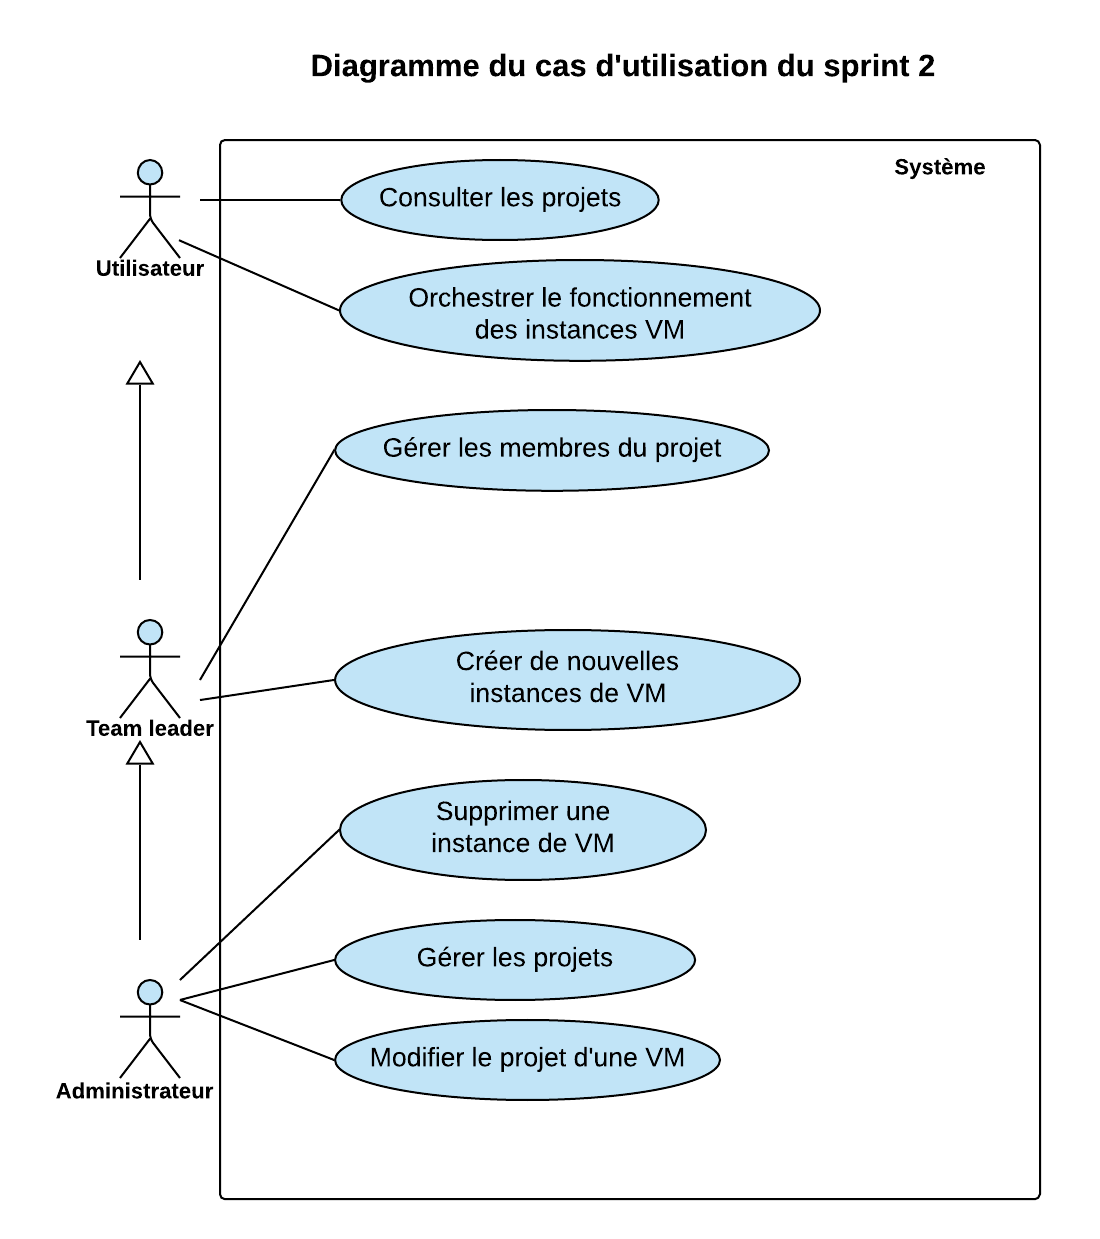
\includegraphics[scale=0.7]{DCUsprint2.png}
	\caption{Diagramme de cas d'utilisation du sprint 2}
	\label{Diagramme de cas d'utilisation du sprint 2}
\end{figure} 
Tel qu'en atteste la figure 4.1, ce sprint permet aux utilisateurs de visualiser leurs projets et les informations appropriées. Ainsi, il les permet d'orchestrer le fonctionnement des instances de machines virtuelles. Encore plus, durant cette itération, le Team leader est apte à créer de nouvelles instances de   machines virtuelles.  Quant à l'administrateur, de plus que toutes les fonctionnalités déjà citées il serait capable de gérer les projets, de créer et de supprimer les VMs non utilisées.
\section{Management des projets}
Cette section est vouée au management des projets. Celui-ci est constitué par les cas d'utilisation "gérer les projets","visualiser les projets" et "gérer les membres du projet".
\subsection{Analyse }
Pour mieux assimiler les cas d'utilisation de la première partie de ce sprint, nous allons définir, dans cette section, leurs raffinements en fournissant une description sur les scénarios.
\begin{itemize}
	\item \textbf{Raffinement du cas d'utilisation "Gérer les membres du projet"} \\
\end{itemize} 
\begin{figure}[H]
	\centering
	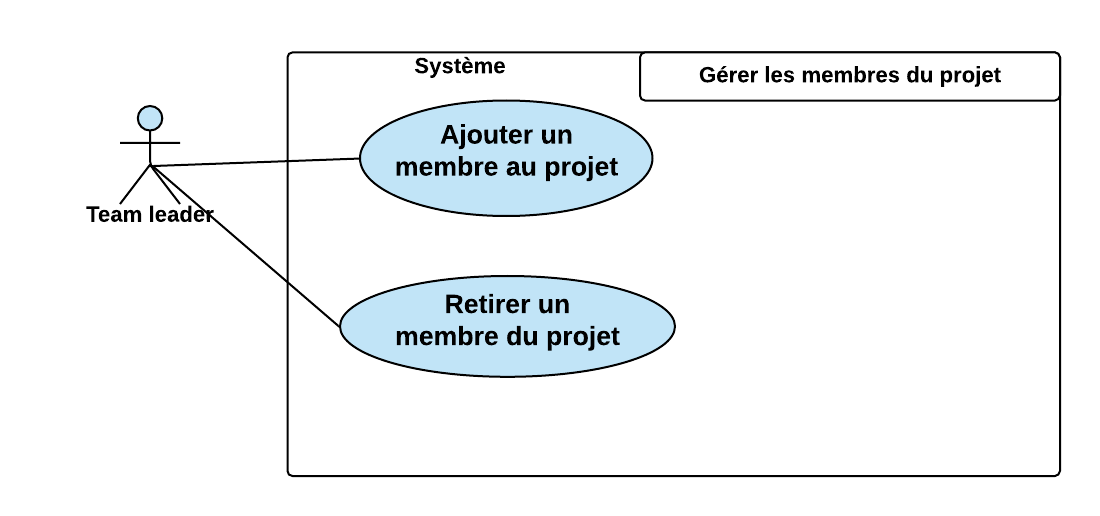
\includegraphics[ height=5cm, width=14cm]{Rgerermembre.png}
	\caption{Raffinement du cas d'utilisation: Gérer les membres du projet}
	\label{Raffinement du cas d'utilisation: Gérer les membres du projet}
\end{figure} 
% Insérer diagramme
Le diagramme de la figure 4.3 ci dessus, présente les sous cas d'utilisation qui étendent de "Gérer les membres du projet".
\subsubsection{Description textuelle du sous cas d'utilisation: "Ajouter un membre au projet"}
% Please add the following required packages to your document preamble:
% \usepackage{multirow}
\begin{table}[H]
	\begin{tabular}{|l|l|}
		\hline
		\textbf{Acteur}                               & Team leadder                                                                                                                             \\ \hline
		\textbf{Description}                          & Ajouter un nouveau membre au projet.                                                                                                    \\ \hline
		\textbf{Préconditions}                        & Team leader authentifié.                                                                                                                 \\ \hline
		\textbf{Post-conditions}                      & Membre ajouté.                                                                                                                           \\ \hline
		\multirow{4}{*}{\textbf{Scénario principal}}  & \begin{tabular}[c]{@{}l@{}}1. Le Team leader remplit les champs relatifs à l'affectation\\ d'un nouveau membre puis valide.\end{tabular} \\ \cline{2-2} 
		& 2. Le système vérifie l'existence de l'utilisateur saisit.                                                                               \\ \cline{2-2} 
		& 3. Le système enregistre le membre ajouté.                                                                                               \\ \cline{2-2} 
		& 4. Le système affiche  la liste des membres mises à jour.                                                                                \\ \hline
		\multirow{2}{*}{\textbf{Scénario altérnatif}} & \begin{tabular}[c]{@{}l@{}}1.a Le Team leader saisit un mail d'utilisateur inexistant\\  dans le système.\end{tabular}                   \\ \cline{2-2} 
		& 1.b Le système affiche un message d'erreur.                                                                                              \\ \hline
	\end{tabular}

\caption{Description textuelle du << Ajouter un membre au projet  >> }
\label{Description textuelle du << Ajouter un membre au projet >>}
\end{table}

\begin{itemize}
	\item \textbf{Raffinement du cas d'utilisation "Gérer les projets"} \\
\end{itemize} 

		\begin{figure}[H]
		\centering
		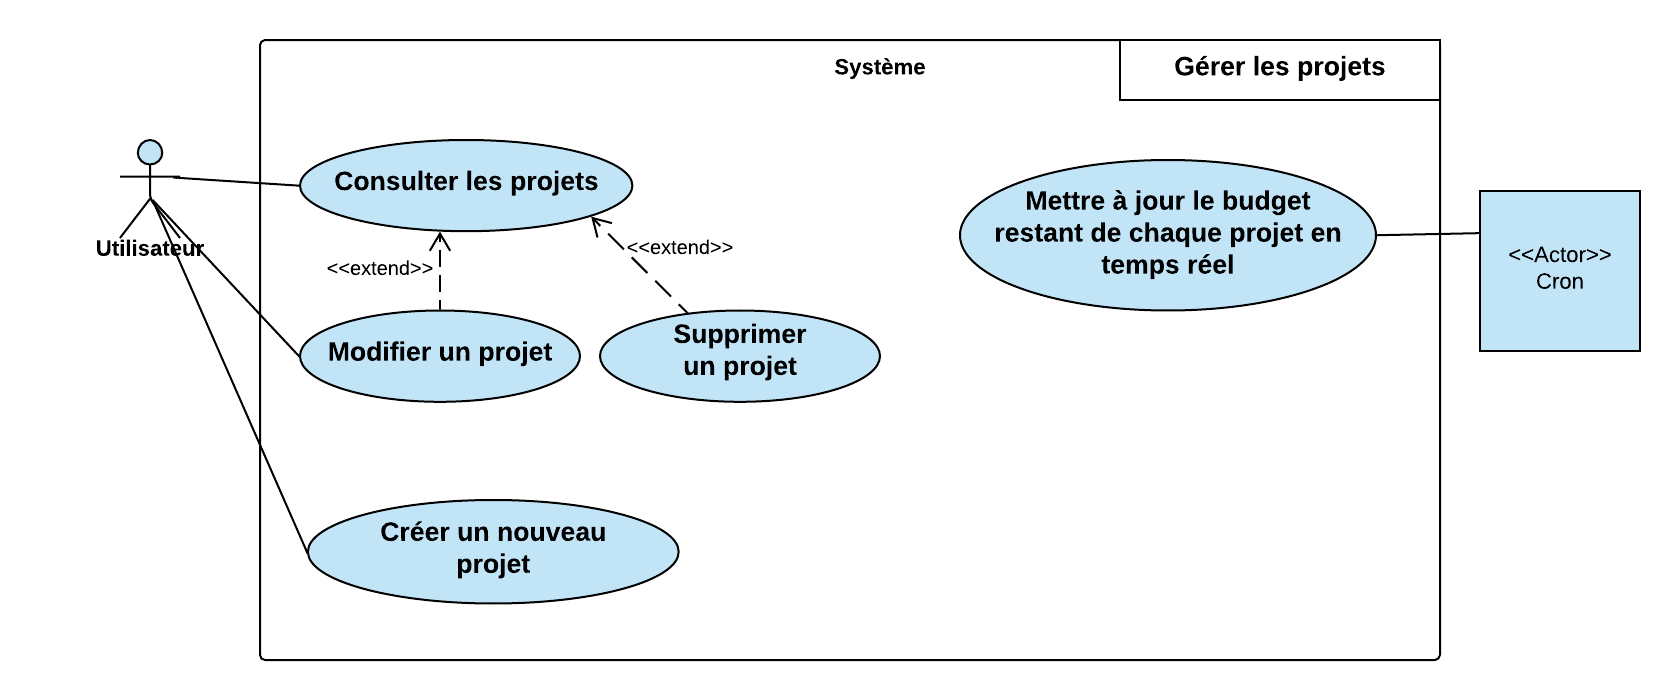
\includegraphics[ height=5.5cm, width=14cm]{Rgererprojet.png}
		\caption{Raffinement du cas d'utilisation: Gérer les projets}
		\label{Raffinement du cas d'utilisation: Gérer les projets}
	\end{figure} 
	Le diagramme de la figure 4.3 représente un raffinement relatif
au cas d'utilisation "gérer  les projets". En effet, ce cas d'utilisation fait intervenir deux acteurs. L'administrateur pour la création d'un nouveau projet et/ou  la consultation de la liste des projets et le Cron pour la mise à jour automatique  du budget restant de chaque projet. \\
En consultant la liste des projets, l'administrateur a la possibilité de modifier ou de supprimer un projet.
\subsubsection{Description textuelle du sous cas d'utilisation: "Créer un nouveau projet"}

% Please add the following required packages to your document preamble:
% \usepackage{multirow}
\begin{table}[H]
	\begin{tabular}{|l|l|}
		\hline
		\textbf{Acteur}                              & Administrateur                                                                                                                           \\ \hline
		\textbf{Description}                         & Ajouter un projet au système.                                                                                                            \\ \hline
		\textbf{Préconditions}                       & Administrateur authentifié.                                                                                                              \\ \hline
		\textbf{Post-conditions}                     & Projet créé.                                                                                                                             \\ \hline
		\multirow{3}{*}{\textbf{Scénario principal}} & \begin{tabular}[c]{@{}l@{}}1. L'administrateur remplit les champs relatifs à la création\\ d'un nouveau projet puis valide.\end{tabular} \\ \cline{2-2} 
		& 2. Le système vérifie l'unicité de projet.                                                                                               \\ \cline{2-2} 
		& 3. Le système ajoute le nouveau projet.                                                                                                  \\ \hline
		\textbf{Scénario altérnatif}                 & \begin{tabular}[c]{@{}l@{}}2.a Le système affiche un message d'erreur indiquant \\ l'existence d'un sujet pareil.\end{tabular}           \\ \hline
	\end{tabular}

\caption{Description textuelle du << Créer un nouveau projet >> }
\label{Description textuelle du << Créer un nouveau projet >>}
\end{table}


\subsection{Conception}
Dans ce qui suit, nous allons détailler et décortiquer les cas d'utilisation les plus prioritaires, de la première partie de ce sprint, à travers les diagrammes de séquences objet.
\subsubsection{Diagramme de séquence du cas d'utilisation: "Mettre à jour  le budget restant de chaque projet en temps réel"}

\begin{figure}[H]
	\centering
	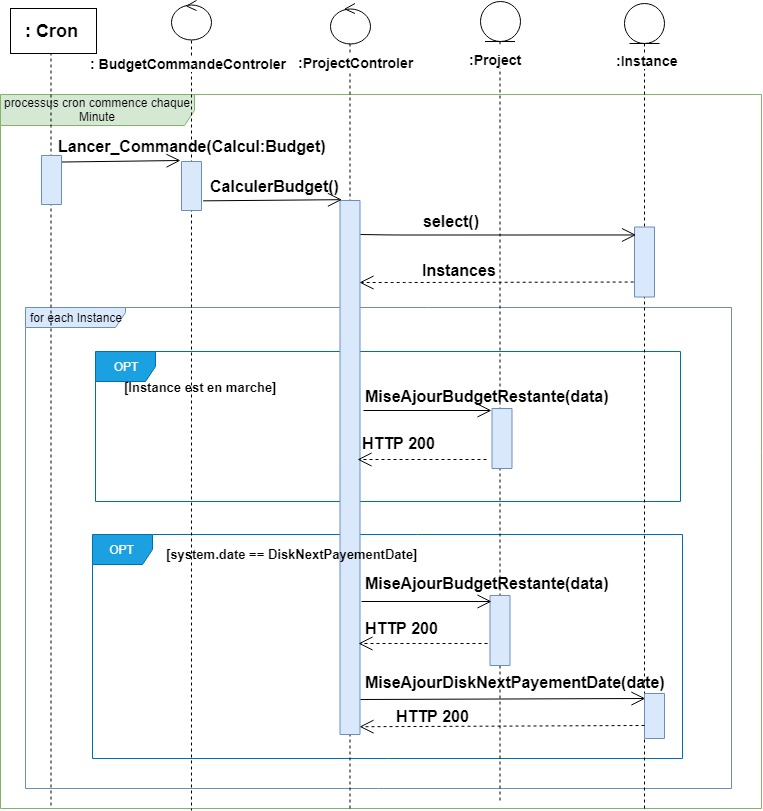
\includegraphics[scale=0.54]{budget2.jpg}
	\caption{Diagramme de séquence: Mettre à jour le budget restant du projet en temps réel }
	\label{Diagramme de séquence: Mettre à jour le budget restant du projet en temps réel }
\end{figure}
Le diagramme de la figure 4.4 détaille la procédure de mise à jour automatique du budget restant de chaque projet. Tout d'abord, Cron lance la commande responsable à la consommation de l'API permettant de calculer le budget restant. Cette opération se répète périodiquement chaque minute. En effet  
cet API consiste à sélectionner toutes les instances de VM et  de faire deux tests pour chaque instance. 
Le premier consiste à vérifier l'état de la machine, si elle est en marche. Le budget restant sera mis à jour. 
Le second consiste à vérifier les dates de système et du prochain payement. S'ils coïncident  le contrôleur  met à jour le budget restant et la date du prochain payement.  Vu que le payement du disque ne s'effectue qu'une seule fois par mois.    
\section{Management des VMs}
Cette section est vouée au management des instances de machines virtuelles qui sont une entité phare dans notre projet. Celui-ci est constitué par les cas d'utilisation "Orchestrer les instances de VM","Créer de nouvelles instances de VM" , "Supprimer une VM" et "Modifier le projet d'une VM".\\
Toutes les taches de cette partie nécessite une préalable configuration au près du Google Cloud plateform pour autoriser l'émission des requêtes à partir de notre application.
\subsection{Analyse}
Dans ce qui suit, nous allons offrir une vue d'ensemble des différentes fonctionnalités
relatives à la deuxième partie de ce sprint. Ensuite, nous allons raffiner et décrire les cas
d'utilisation les plus prioritaires.
\begin{itemize}
	\item \textbf{Raffinement du cas d'utilisation "Orchestrer les instances de VM"}
	 
		\begin{figure}[H]
		\centering
		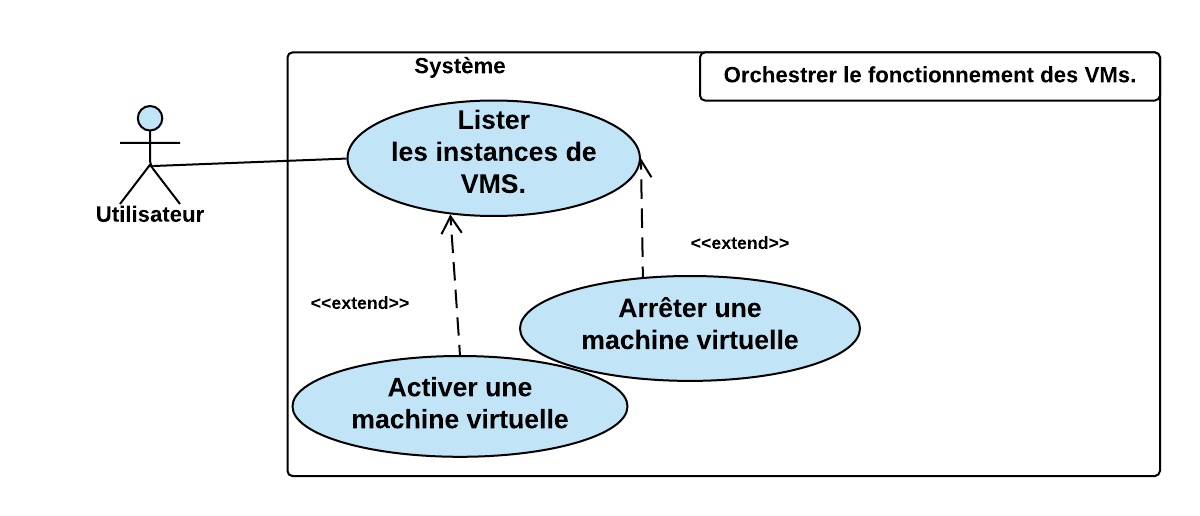
\includegraphics[ height=4cm, width=14cm]{Rorchestrer.png}
		\caption{Raffinement du cas d'utilisation: Orchestrer le fonctionnement des VMs}
		\label{Raffinement du cas d'utilisation: Orchestrer le fonctionnement des VMs}
	\end{figure} 
\end{itemize}
	Le diagramme de cas d'utilisation de la figure 4.5 met en évidence un raffinement lié
au cas d'utilisation "Orchestrer le fonctionnement des VMs". Cette opération est assurée à travers la consultation de la liste des machines virtuelles ou l'utilisateur peut  activer ou arrêter une VM.
\subsubsection{Description textuelle du cas d'utilisation: "Lister les instances de VM"}

% Please add the following required packages to your document preamble:
% \usepackage{multirow}
\begin{table}[H]
	\begin{tabular}{|l|l|}
		\hline
		\textbf{Acteur}                               & Utilisateur.                                                                                                                         \\ \hline
		\textbf{Description}                          & Récupérer les instances de VM                                                                                                        \\ \hline
		\textbf{Préconditions}                        & 1.Utilisateur authentifié.                                                                                                           \\ \hline
		\textbf{Post-conditions}                      & Liste des instances de VM récupérée.                                                                                                 \\ \hline
		\multirow{3}{*}{\textbf{Scénario principal}}  & 1. L'utilisateur demande l'accès à la liste des  instances de VM.                                                                       \\ \cline{2-2} 
		& \begin{tabular}[c]{@{}l@{}}2. Le système récupère la liste des projets auquel appartient\\ l'utilisateur courant.\end{tabular}       \\ \cline{2-2} 
		& \begin{tabular}[c]{@{}l@{}}3. Le système affiche la liste des instances de VM des projets\\ retournés\end{tabular}                   \\ \hline
		\multirow{2}{*}{\textbf{Scénario altérnatif}} & 2.a L'utilisateur n'appartient à aucun projet.                                                                                       \\ \cline{2-2} 
		& \begin{tabular}[c]{@{}l@{}}2.b Le système affiche un message indiquant que l'utilisateur\\ n'appartient à aucun projet.\end{tabular} \\ \hline
	\end{tabular}

\caption{Description textuelle du << Lister les instances de VM >> }
\label{Description textuelle du << Lister les instances de VM >>}
\end{table}

\subsubsection{Description textuelle du sous cas d'utilisation: "Activer une machine virtuelle"}
% Please add the following required packages to your document preamble:
% \usepackage{multirow}
\begin{table}[H]
	\begin{tabular}{|l|l|}
		\hline
		\textbf{Acteur}                               & Utilisateur.                                                                                                              \\ \hline
		\textbf{Description}                          & Activer une machine virtuelle.                                                                                            \\ \hline
		\multirow{2}{*}{\textbf{Préconditions}}       & 1.Utilisateur authentifié.                                                                                                \\ \cline{2-2} 
		& 2. Requetes autorisées.                                                                                                   \\ \hline
		\textbf{Post-conditions}                      & Machine virtuelle activée.                                                                                                \\ \hline
		\multirow{4}{*}{\textbf{Scénario principal}}  & 1. L'utilisateur clique sur le bouton d'activation d'une VM.                                                              \\ \cline{2-2} 
		& 2. Le système récupère le  budget restant du projet de la VM                                                              \\ \cline{2-2} 
		& \begin{tabular}[c]{@{}l@{}}3. Le système demande au serveur du Google Compute engine\\ d'activer la VM.\end{tabular}      \\ \cline{2-2} 
		& \begin{tabular}[c]{@{}l@{}}4. Le système met à jour l'état de la VM dans la base de \\ données.\end{tabular}              \\ \hline
		\multirow{2}{*}{\textbf{Scénario altérnatif}} & \begin{tabular}[c]{@{}l@{}}2.a Le budget restant du projet insuffisant pour démarrer une \\ VM.\end{tabular}              \\ \cline{2-2} 
		& \begin{tabular}[c]{@{}l@{}}2.b Le système affiche un message d'erreur indiquant \\ l'insuffisance du budget.\end{tabular} \\ \hline
	\end{tabular}

\caption{Description textuelle du << Activer une machine virtuelle >> }
\label{Description textuelle du << Activer une machine virtuelle >>}
\end{table}

\subsection{Conception}
Afin de décortiquer et détailler les cas d'utilisation précédemment cités, nous présentons dans ce qui suit les diagrammes de séquences des cas d'utilisation les plus importants
\subsubsection{Diagramme de séquence du cas d'utilisation: "Créer une nouvelle instance de VM"}

\begin{figure}[H]
	\centering
	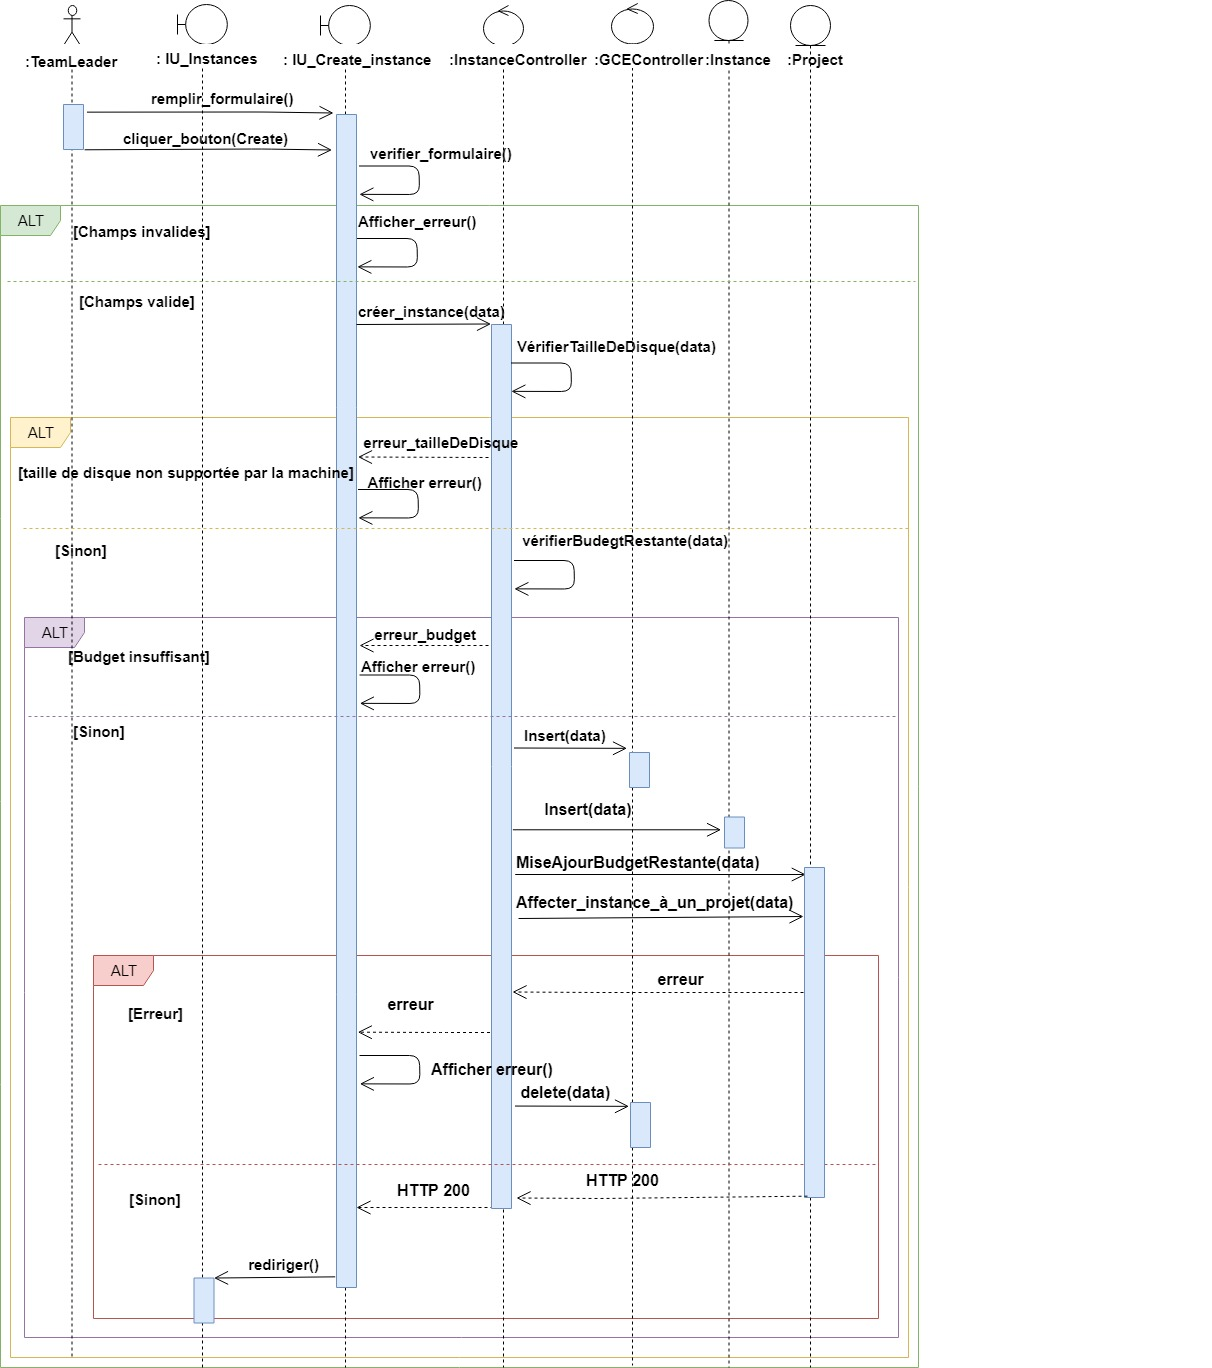
\includegraphics[ height=18cm, width=20cm]{createInstance-Page-1.jpg}
	\caption{Diagramme de séquence: Créer une nouvelle instance de VM}
	\label{Diagramme de séquence: Créer une nouvelle instance de VM}
\end{figure}
Le diagramme de la figure 4.6 illustre la procédure de création d'une instance de machine virtuelle. Tout d'abord, le Team leader remplit le formulaire  puis valide et confirme. Une fois confirmé, 
le contrôleur  vérifie la compatibilité entre la taille du disque et le type de la machine émis. S'ils sont incompatibles le contrôleur retourne une erreur, sinon il vérifie le budget restant du projet. S'il est suffisant pour créer une VM le contrôleur demande au serveur du Google Compute Engine de créer la VM puis il l'insère dans l'entité Instance et met à jour le projet associé et son budget restant. Dans le cas ou une erreur s'est produite au niveau de l'insertion dans la base de données, le contrôleur annule l'opération en supprimant la VM de la part de Google Compute Engine afin d'assurer la synchronisation.

\subsubsection{Diagramme de séquence du cas d'utilisation: "Modifier le projet d'une machine virtuelle"}

\begin{figure}[H]
	\centering
	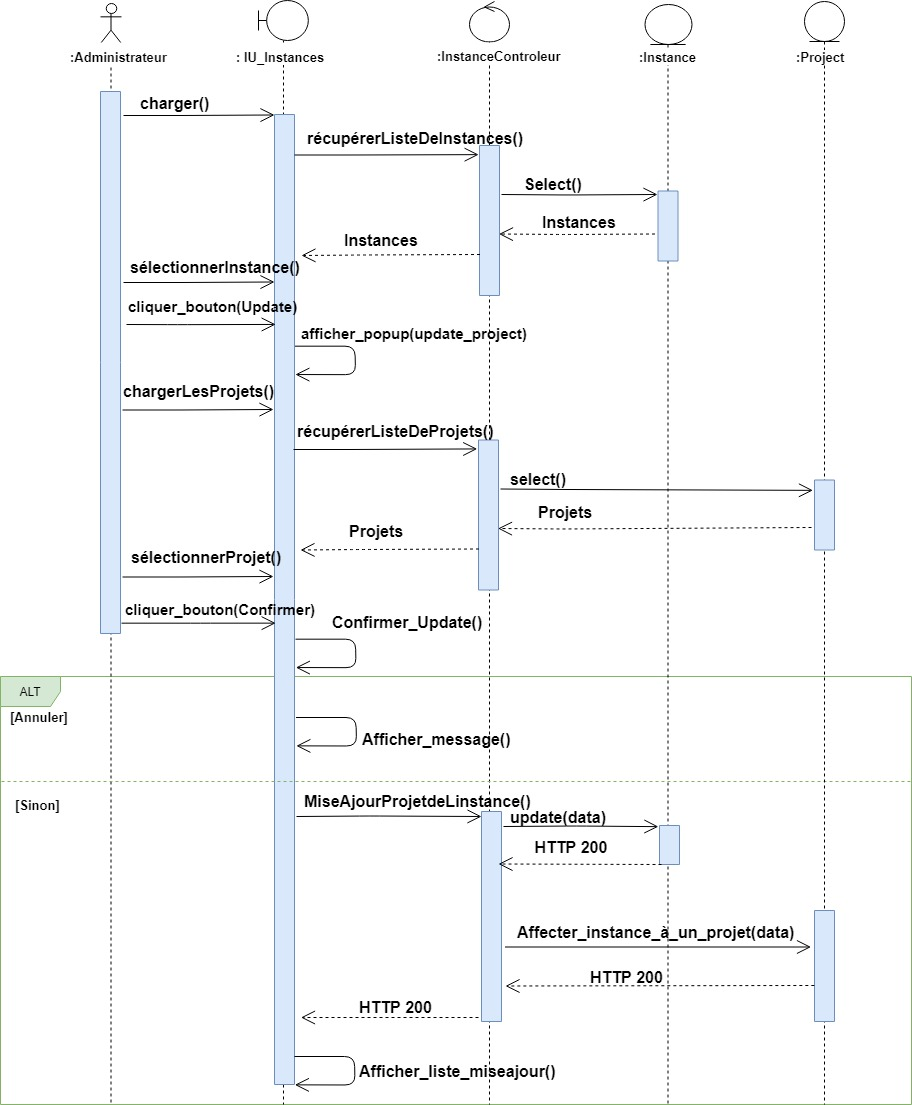
\includegraphics[scale=0.4]{updateProjectOfisntate.jpg}}
	\caption{Diagramme de séquence: Modifier le projet d'une machine virtuelle }
	\label{Diagramme de séquence: Modifier le projet d'une machine virtuelle }
\end{figure}

Le diagramme de la figure 3.8 décrit l'opération de modification du projet d'une machine virtuelle. Tout
d'abord, l'administrateur récupère toutes les instances de machine virtuelle. Ensuite, Il sélectionne la machine virtuelle adéquate et choisit le  nouveau projet  puis valide. Une fois validé, une modale de confirmation s'ouvre. Là ou
il peut soit annuler l'opération, soit la confirmer. S'il confirme 
les données nécessaires à la modification seront émises au contrôleur des instances pour effectuer les changements dans les entités Instance et projet. Finalement le contrôleur retourne une requête Htp de
statut 200 en cas de succès.

\section{Réalisation}
Passons à la partie réalisation, nous allons capturer quelques interfaces de ce deuxième 
sprint.
\subsection{Interfaces}
	\begin{figure}[H]
	\centering
	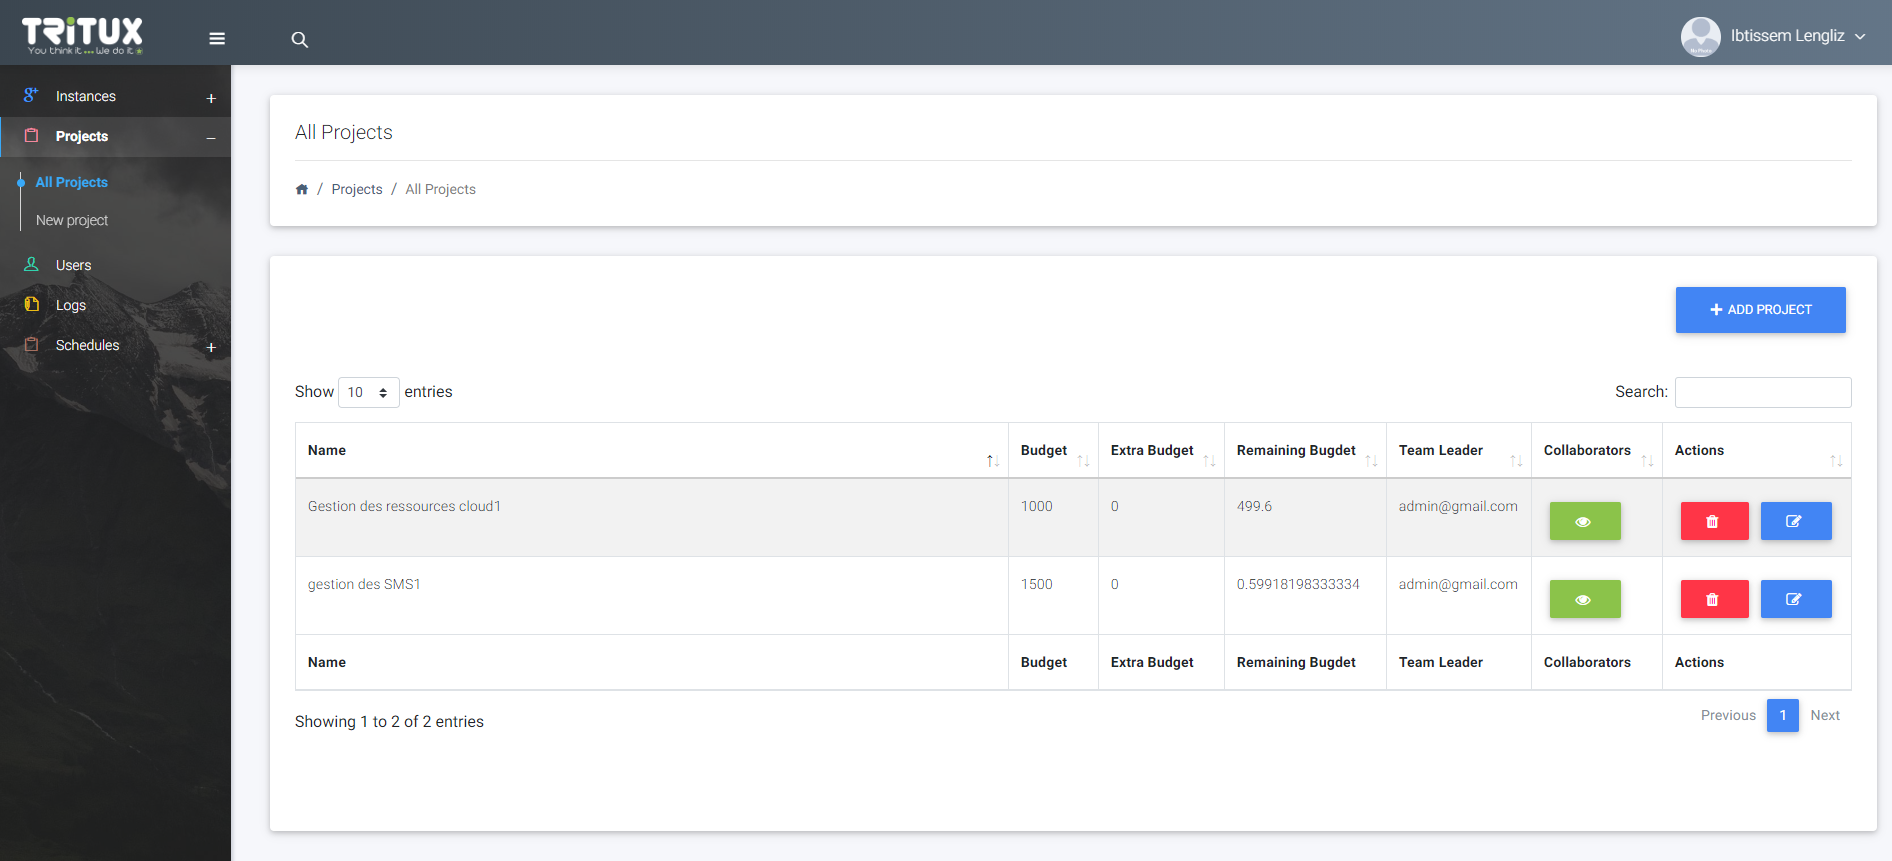
\includegraphics[scale=0.35]{projets.PNG}
	\caption{Interface de gestion des projets}
	\label{Interface de gestion des projets}
\end{figure}

La figure 4.8 représente l'interface de gestion des projets, grâce à laquelle l'administrateur
pourra rechercher , supprimer , modifier un projet et  créer un nouveau projet comme le montre la figure 4.9 ci-dessous. 
	\begin{figure}[H]
	\centering
	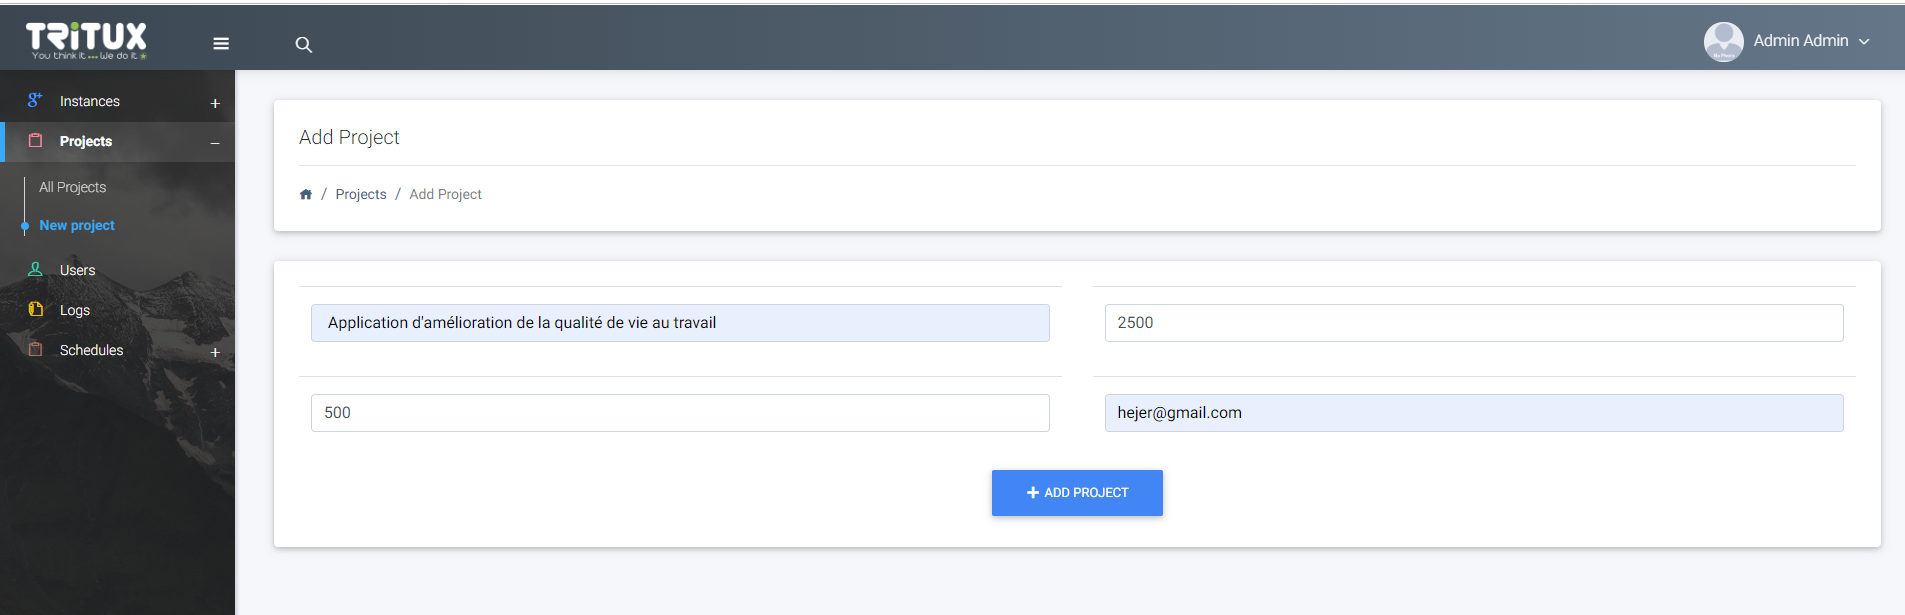
\includegraphics[scale=0.35]{addproject.PNG}
	\caption{Interface de création d'un nouveau projet}
	\label{Interface de création d'un nouveau projet}
\end{figure}

	\begin{figure}[H]
	\centering
	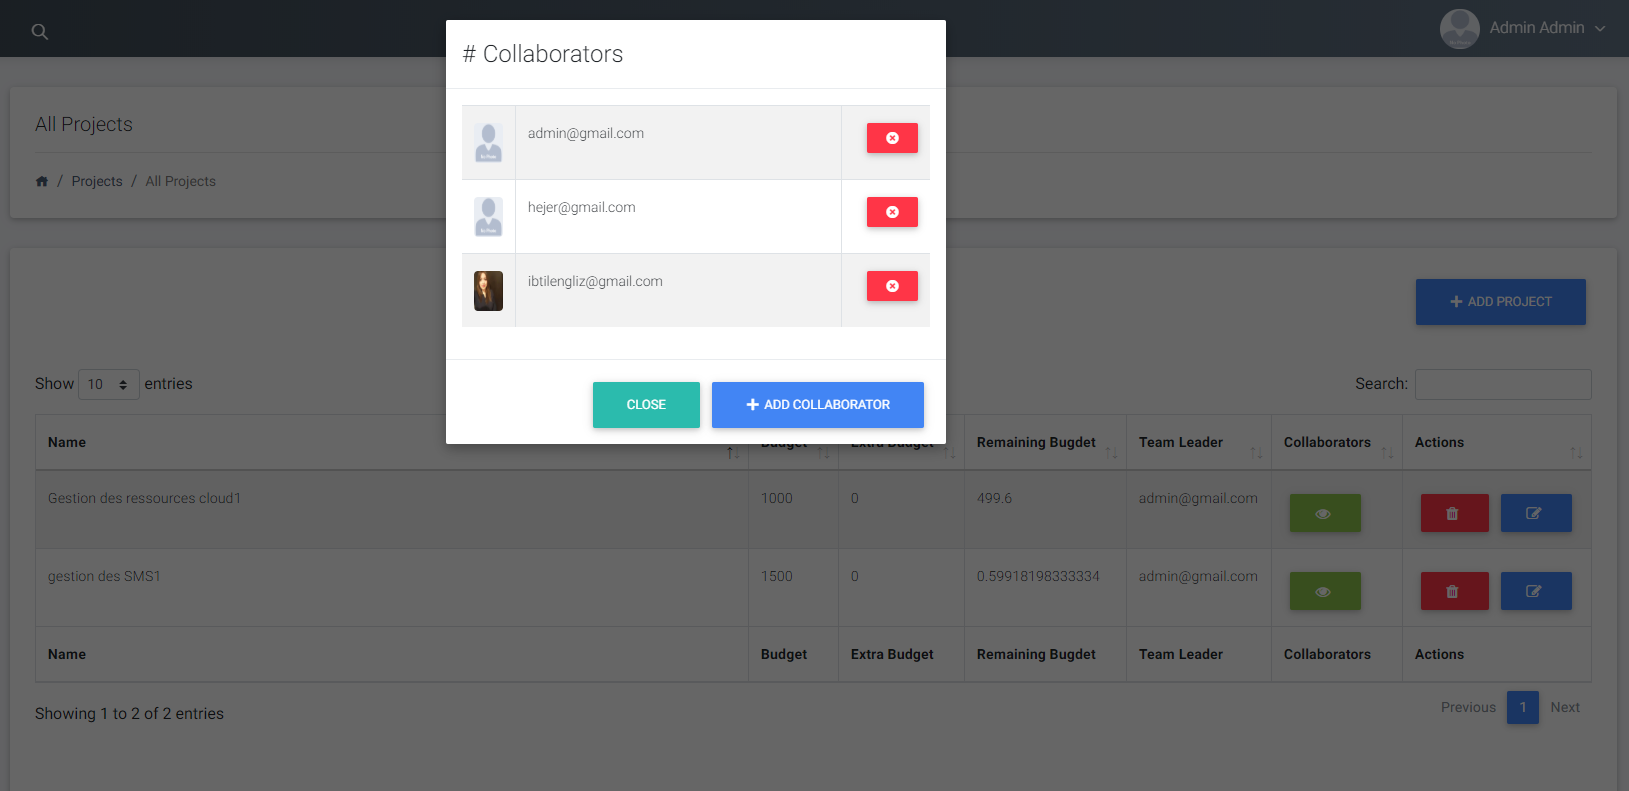
\includegraphics[scale=0.35]{membreProjets.PNG}
	\caption{Interface de gestion des membres du projet}
	\label{Interface de gestion des membres du projet}
\end{figure}
La figure 4.10 ci dessus met en évidence la gestion des membres du projet. Dedans, le team leader peut affecter ou retirer des collaborateurs.
\begin{figure}[H]
	\centering
	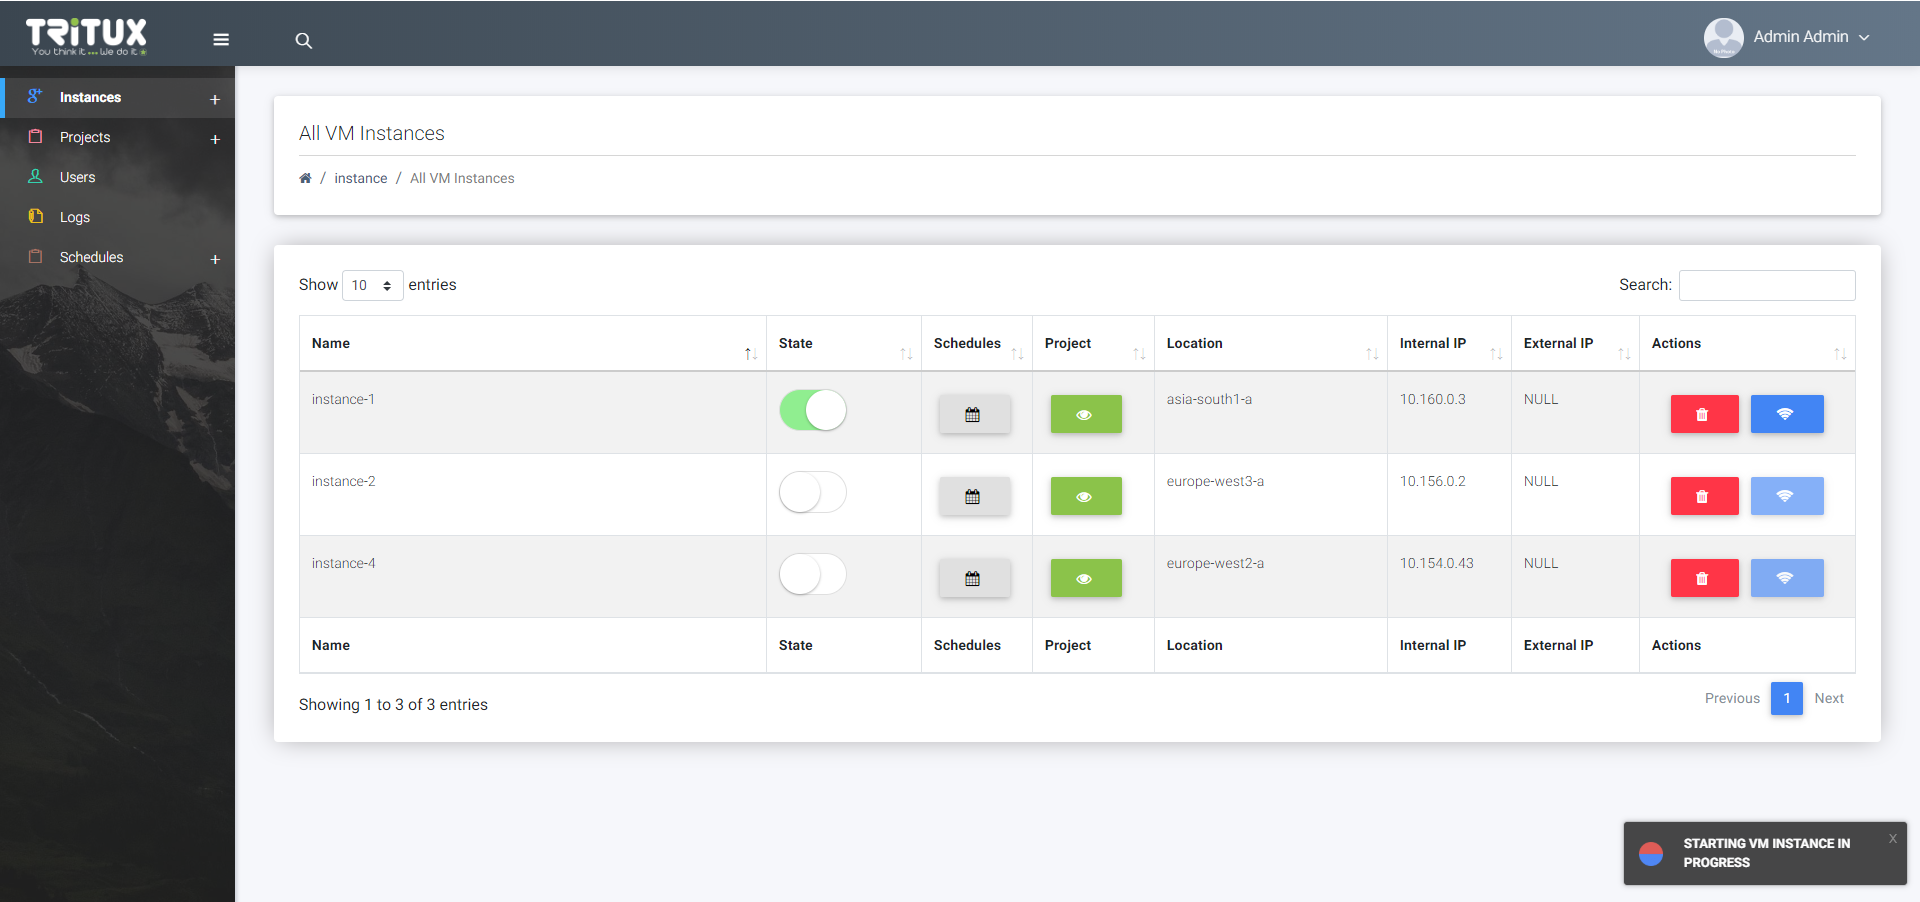
\includegraphics[scale=0.273]{instances.png}
	\caption{Interface de gestion des instances de machine virtuelle}
	\label{Interface de gestion des instances de machine virtuelle}
\end{figure}

La figure 4.11 représente l'interface de gestion des machines virtuelles, grâce à laquelle l'administrateur
pourra rechercher , supprimer , orchestrer le fonctionnement des VMs , affecter un planning, modifier le projet de chaque VM et créer une machine virtuelle comme le montre la figure 4.12. 
Ce dernier il peut aussi consulter les détails de chaque instance de machine virtuelle grâce à la figure 4.13.

\begin{figure}[H]
	\centering
	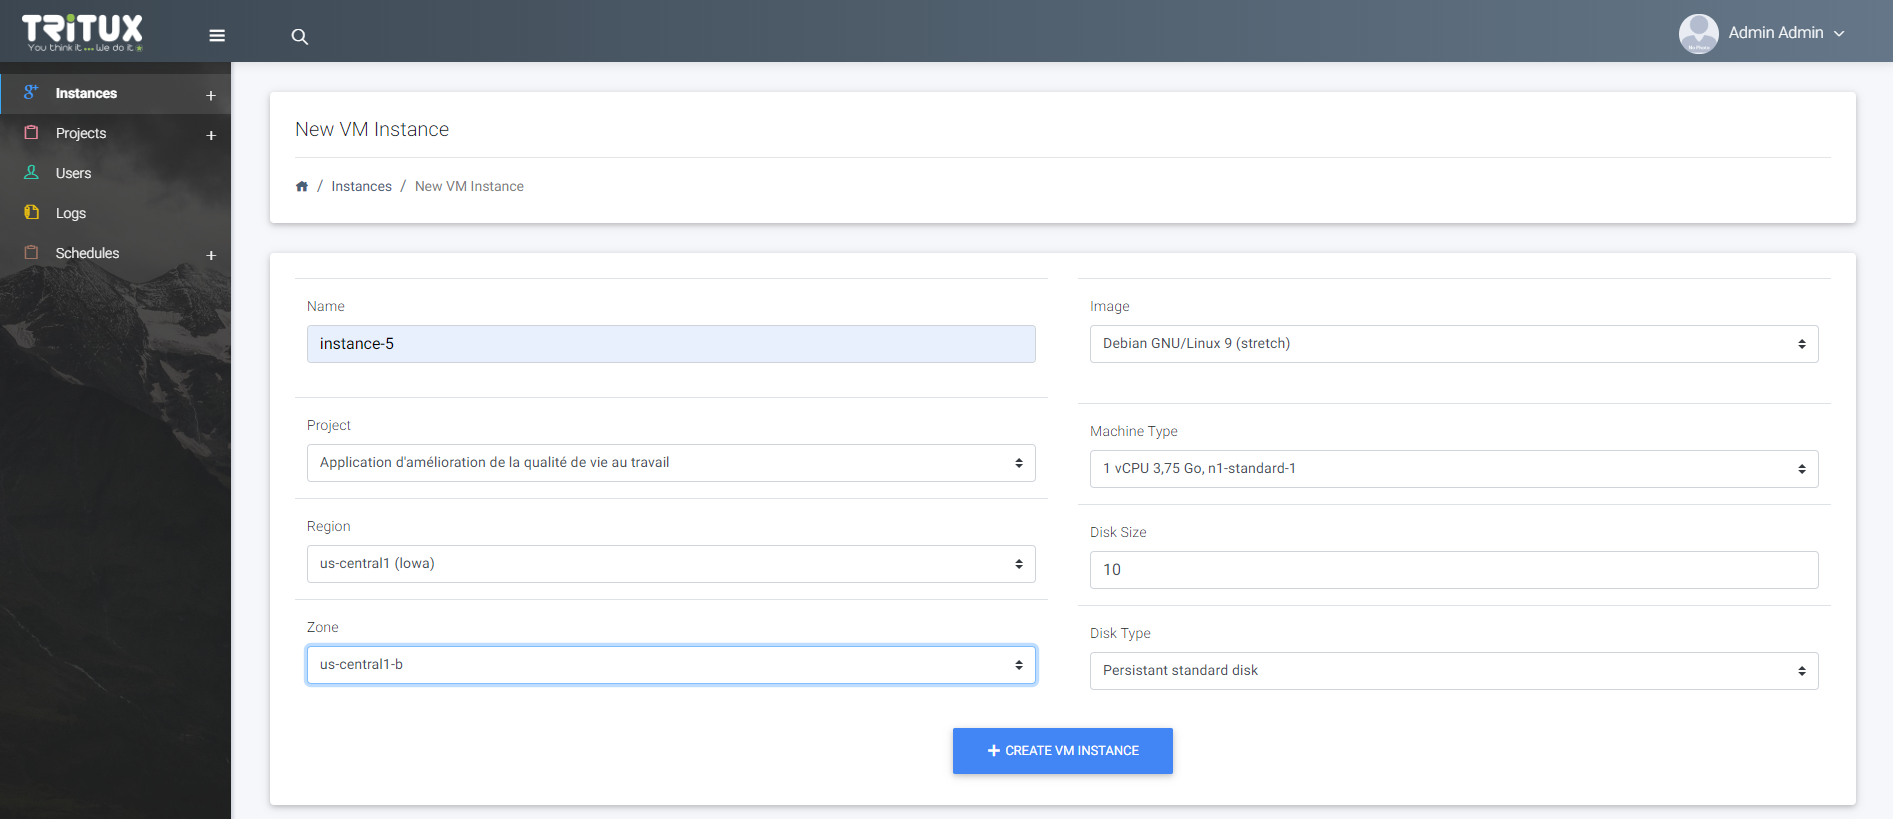
\includegraphics[scale=0.35]{createvm.png}
	\caption{Interface de création d'une nouvelle instance de machine virtuelle}
	\label{Interface de création d'une nouvelle instance de machine virtuelle}
\end{figure}
\begin{figure}[H]
	\centering
	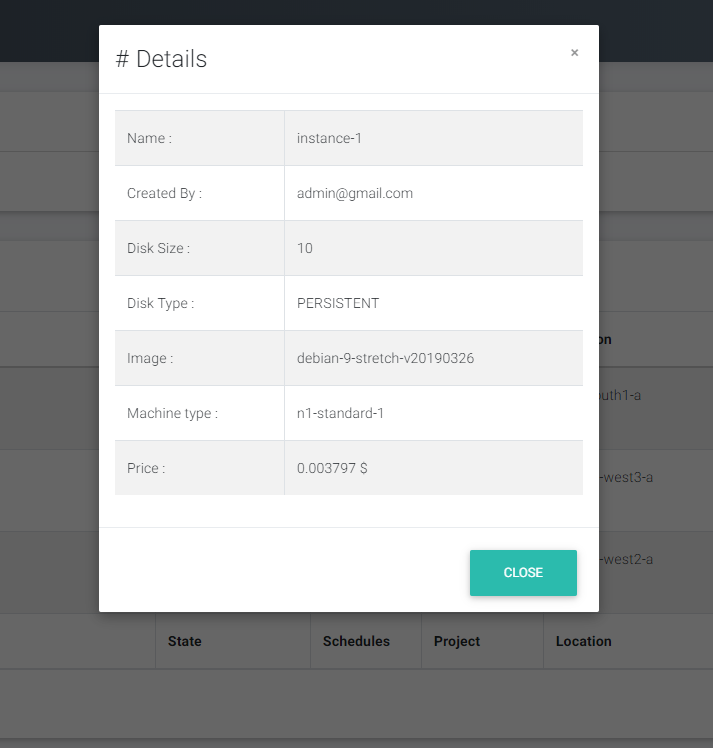
\includegraphics[scale=0.35]{details.PNG}
	\caption{Interface de détails des instances de machine virtuelle}
	\label{Interface des détails des instances de machine virtuelle}
\end{figure}

\section{Conclusion}
Au cours de ce sprint nous avons pu détaillé les principaux fonctionnalités  de la partie la plus importante de notre application qui est la gestion des machines virtuelle et des projets. Cette partie met en évidence la contrôle des VMs par projet et son budget. Dans le
chapitre suivant nous allons attaquer avec la même approche le troisième sprint.

\chapter{Sprint3: Gestion des planifications et logs}
\section {Introduction}
L'objectif de ce chapitre est de présenter la dernière itération du cycle de vie de notre
projet. Nous allons entamer par identifier les tâches à réaliser dans le Backlog du Sprint pour
passer par la suite aux phases d'analyse et de conception. Nous finirons par exposer la phase de
réalisation de ce module. \\Nous avons décidé de découper ce sprint en deux parties, une
partie pour la gestion des planifications et une autre partie pour les logs qui permettent à l'administrateur d'avoir une vision globale sur l'activité des utilisateurs.
\section{Etude fonctionnelle}
\subsection{Backlog du Sprint} 
Le Backlog du sprint présentés par le tableau 3.1 contient une liste des tâches de chaque user story identifiées par l'équipe Scrum et qui
devront être réalisées pendant ce sprint.
% Please add the following required packages to your document preamble:
% \usepackage{multirow}
\begin{table}[H]
	\begin{tabular}{|l|l|l|l|}
		\hline
		\textbf{ID}          & \textbf{User Story}                                                                                                                                                     & \textbf{Description}                                                                                                                                                     & \textbf{Esti.} \\ \hline
	
		\multirow{3}{*}{5.1} & \multirow{3}{*}{\begin{tabular}[c]{@{}l@{}}En tant que utilisateur, je souhaite \\ consulter la liste des plannings.\end{tabular}}                                      & \begin{tabular}[c]{@{}l@{}}Créer la "datatable" de \\ sélection de tous les\\  plannings.\end{tabular}                                                                   & 2              \\ \cline{3-4} 
		&                                                                                                                                                                         & \begin{tabular}[c]{@{}l@{}}Créer l'API de sélection \\ des plannings.\end{tabular}                                                                                       & 3              \\ \cline{3-4} 
		&                                                                                                                                                                         & Consommer l'API                                                                                                                                                          & 3              \\ \hline
			\multirow{3}{*}{5.2} & \multirow{3}{*}{\begin{tabular}[c]{@{}l@{}}En tant que utilisateur, je souhaite créer \\ un planning.\end{tabular}}                                                     & \begin{tabular}[c]{@{}l@{}}Implémenter la vue de\\  création d'un planning.\end{tabular}                                                                                 & 5              \\ \cline{3-4} 
		&                                                                                                                                                                         & \begin{tabular}[c]{@{}l@{}}Générer l'API de création\\  d'un planning.\end{tabular}                                                                                      & 4              \\ \cline{3-4} 
		&                                                                                                                                                                         & Consommer l'API.                                                                                                                                                         & 3              \\ \hline	
		\end{tabular}
	\end{table}
\begin{table}[H]
	\begin{tabular}{|l|l|l|l|}
		\hline
		\textbf{ID}          & \textbf{User Story}                                                                                                                                                     & \textbf{Description}                                                                                                                                                     & \textbf{Esti.} \\ \hline
	
		\multirow{3}{*}{5.3} & \multirow{3}{*}{\begin{tabular}[c]{@{}l@{}}En tant que utilisateur,je souhaite \\ supprimer un planning.\end{tabular}}                                                  & \begin{tabular}[c]{@{}l@{}}Créer la modale de \\ confirmation de suppression \\ d'un planning\end{tabular}                                                               & 3              \\ \cline{3-4} 
		&                                                                                                                                                                         & \begin{tabular}[c]{@{}l@{}}Créer l'API de suppression \\ d'un planning.\end{tabular}                                                                                     & 3              \\ \cline{3-4} 
		&                                                                                                                                                                         & Consommer l'API.                                                                                                                                                         & 3              \\ \hline
		\multirow{4}{*}{5.4} & \multirow{4}{*}{\begin{tabular}[c]{@{}l@{}}En tant que utilisateur, je souhaite\\  affecter un planning à une VM.\end{tabular}}                                         & Mettre en place l'outil Cron.                                                                                                                                            & 2              \\ \cline{3-4} 
		&                                                                                                                                                                         & \begin{tabular}[c]{@{}l@{}}Créer la modale de \\ consultation, affectation et \\ de détachement\\ d'un planning d'une VM.\end{tabular}                                   & 5              \\ \cline{3-4} 
		&                                                                                                                                                                         & \begin{tabular}[c]{@{}l@{}}Créer l'API d'affectation \\ d'un planning à une VM.\end{tabular}                                                                             & 4              \\ \cline{3-4} 
		&                                                                                                                                                                         & Consommer l'API.                                                                                                                                                         & 3              \\ \hline
		\multirow{2}{*}{5.5} & \multirow{2}{*}{\begin{tabular}[c]{@{}l@{}}En tant que utilisateur, je souhaite \\ retirer un planning d'une VM.\end{tabular}}                                          & \begin{tabular}[c]{@{}l@{}}Créer l'API de retrait\\  d'un planning d'une VM.\end{tabular}                                                                                & 3              \\ \cline{3-4} 
		&                                                                                                                                                                         & Consommer l'API.                                                                                                                                                         & 3              \\ \hline
		\multirow{3}{*}{6.1} & \multirow{3}{*}{\begin{tabular}[c]{@{}l@{}}En tant que utilisateur, je souhaite \\ consulter les activités des utilisateurs.\end{tabular}}                              & \begin{tabular}[c]{@{}l@{}}Créer la "datatable" \\ de sélection des logs.\end{tabular}                                                                                   & 3              \\ \cline{3-4} 
		&                                                                                                                                                                         & \begin{tabular}[c]{@{}l@{}}Créer l'API de sélection \\ des logs.\end{tabular}                                                                                            & 3              \\ \cline{3-4} 
		&                                                                                                                                                                         & Consommer l'API.                                                                                                                                                         & 3              \\ \hline
	\end{tabular}

\caption{Backlog du Sprint 3}
\label{Backlog  du Sprint 3}
\end{table}



\subsection{Diagramme de cas d'utilisation du sprint 3}
Le diagramme de cas d'utilisation du troisième sprint exposé par la figure 5.1 a pour but d'établir les besoins, les résultats espérés et les mission les plus prioritaires de la troisième valeur métier.\\
Tous les cas d'utilisation de ce sprint sont précédés par une opération d'authentification.\\
\begin{figure}[ht]
	\centering
	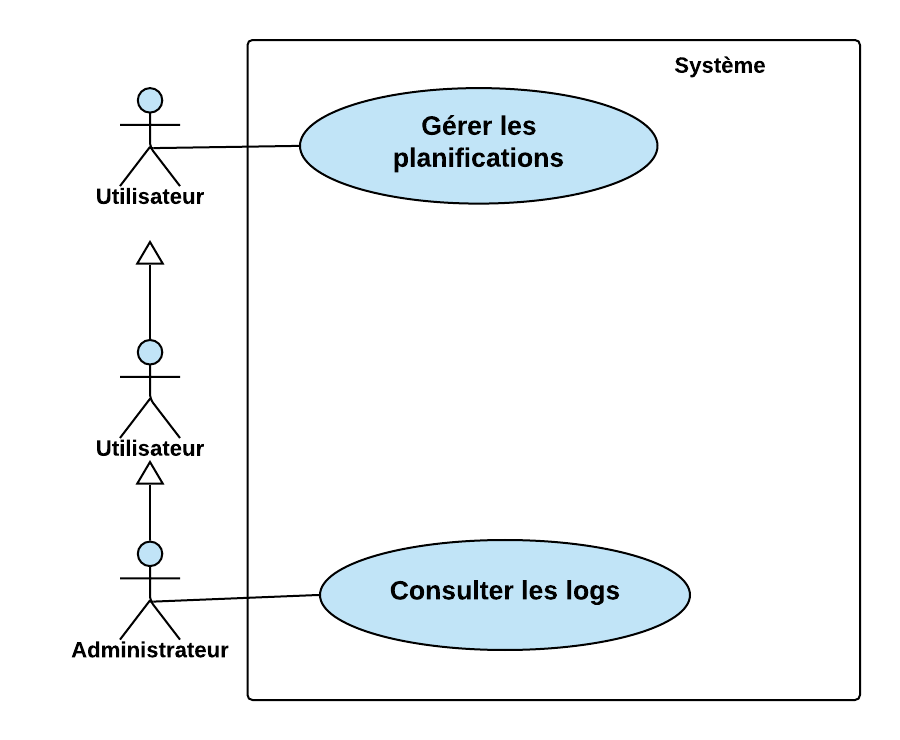
\includegraphics[scale=0.5]{sprint3.png}
	\caption{Diagramme de cas d'utilisation du sprint 3}
	\label{Diagramme de cas d'utilisation du sprint 3}
\end{figure} \\
Tel qu'en atteste la figure 5.1, ce sprint permet aux utilisateurs de gérer les planifications. Ainsi, il  permet à l'administrateur de consulter les logs.
\section{Gestion des planifications }
Cette section est dédiée à la gestion des planifications. Elle est constituée par le cas d'utilisation "Gérer les planifications".\\
 La réalisation de ce cette partie nécessite l'utilisation du planificateur de tâches Cron. Ce dernier 
 est un utilitaire linux  qui planifie l'exécution automatique d'une commande ou d'un script sur le serveur à une date et une heure spécifiées. Il est utile pour automatiser  des tâches répétitives.
 Dans notre cas, il va planifier le fonctionnement des machines virtuelles.
\subsection{Analyse}
Afin de mieux  détailler le fonctionnement et assimiler les cas d'utilisation de ce sprint, nous allons établir, dans cette section,  leurs raffinements en livrant une description sur les scénarios les plus importants.
\begin{itemize}
	\item \textbf{Raffinement du cas d'utilisation "Gérer les planifications"}
\end{itemize}
\begin{figure}[h]
	\centering
	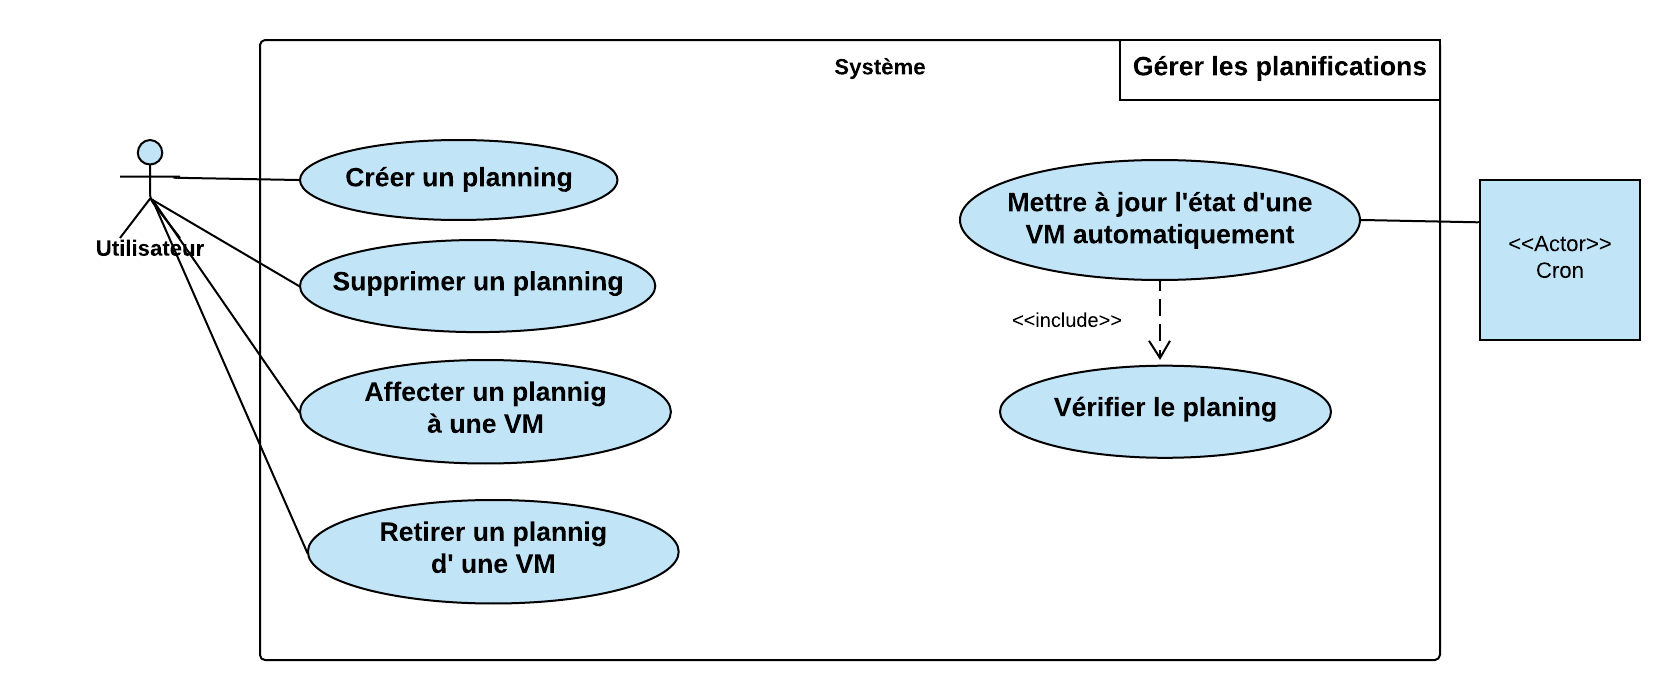
\includegraphics[ height=5.1cm, width=14cm]{Rgererplani.png}
	\caption{Raffinement du cas d'utilisation: Gérer les planifications}
	\label{Raffinement du cas d'utilisation: Gérer les planifications}
\end{figure} 
Comme le montre la figure 5.2, la création, suppression d'un planning et son  retrait  et affectation  à une VM sont tous des sous cas d'utilisation qui s'étendent de la gestion des planifications. En outre, la mise à jour automatique de l'état de la VM avec une vérification du planning affecté sont des cas d'utilisations assurés à travers notre second acteur qui est le Cron.

\subsubsection{Description textuelle du cas d'utilisation: "Supprimer un planning}

% Please add the following required packages to your document preamble:
% \usepackage{multirow}
\begin{table}[ht]
	\begin{tabular}{|l|l|}
		\hline
		\textbf{Acteur}                              & Utilisateur                                                                                                                \\ \hline
		\textbf{Description}                         & Supprimer un planning.                                                                                                     \\ \hline
		\textbf{Préconditions}                       & Utilisateur authentifié                                                                                                    \\ \hline
		\textbf{Post-conditions}                     & Planning supprimé.                                                                                                         \\ \hline
		\multirow{4}{*}{\textbf{Scénario principal}} & \begin{tabular}[c]{@{}l@{}}1. L'utilisateur sélectionne le planning et clique sur le bouton\\ de suppression.\end{tabular} \\ \cline{2-2} 
		& 2. Le système affiche une modale de confirmation.                                                                          \\ \cline{2-2} 
		& 3. L'utilisateur confirme son choix.                                                                                       \\ \cline{2-2} 
		& 4.  Le système supprime le planning correspondant.                                                                         \\ \hline
		\textbf{Scénario altérnatif}                 & 2.a L'utilisateur décide d'annuler son choix.                                                                              \\ \hline
	\end{tabular}

\caption{Description textuelle du << Supprimer un planning >> }
\label{Description textuelle du << Supprimer un planning >>}
\end{table}

\subsection{Conception}

Afin de décortiquer et détailler les cas d'utilisation précédemment cités, nous présentons dans ce qui suit les diagrammes de séquences des cas d'utilisation les plus importants
\subsubsection{Diagramme de séquence du cas d'utilisation: "Mettre à jour l'état d'une machine virtuelle automatiquement"}

\begin{figure}[H]
	\centering
	\includegraphics[ height=15cm, width=15cm]{schedule1.jpg}
	\caption{Diagramme de séquence: Mettre à jour l'état d'une machine virtuelle automatiquement}
	\label{Diagramme de séquence: Mettre à jour l'état d'une machine virtuelle automatiquement}
\end{figure}
Le diagramme de la figure 5.3 détaille la procédure relative à la mise  à jour automatique de l'état des VMs. Cette opération nécessite la mise en place de l'outil Cron de linux.
Chaque heure, cron demande la consommation de l'API responsable au fonctionnement  automatique des machines virtuelles. Au moment de l'exécution de cet API, le contrôleur des planifications récupère la liste des instances et pour chaque instance qui a un planning il vérifie  si elle est en état de repos et si son planning l'oblige pour qu'elle soit activée. Si c'est le cas,  le contrôleur émet une requête au Google Compute engine  pour l'activer et une  autre pour changer son état  dans la base de données. Dans le cas ou une erreur s'est produite au niveau de la mise à jour dans la base de données et pour en assurer la synchronisation le contrôleur annule l'opération en arrêtant la VM auprès de Google Compute Engine. 
Pareil pour l'arrêt automatique d'une machine mise en marche.
\subsubsection{Diagramme de séquence du cas d'utilisation: "Créer un planning"}

\begin{figure}[H]
	\centering
	\includegraphics[scale=0.6]{createSchedule.png}
	\caption{Diagramme de séquence: Créer un planificateur}
	\label{Diagramme de séquence: Créer un planificateur}
\end{figure}
Le diagramme de la figure décrit l'opération de création d'un planning. Tout d'abord, l'utilisateur remplit le formulaire correspondant et choisit l'horaire du fonctionnement de  la machine virtuelle puis valide. Une fois validé, le contrôleur émet une requête de création d'un planning. Il retourne une requête de statut 200 si la création est effectuée avec succès et une erreur dans le cas contraire.
\section{Gestion des logs }
Cette section est dédiée à la gestion des logs. Elle est constituée par le cas d'utilisation "Consulter les logs".\\

\subsection{Analyse}
Dans ce qui suit, nous allons offrir une vue d'ensemble des fonctionnalités
relatives à la deuxième partie de ce sprint. 
\subsubsection{Description textuelle du cas d'utilisation: "Consulter les logs"}
% Please add the following required packages to your document preamble:
% \usepackage{multirow}
\begin{table}[H]
	\begin{tabular}{|l|l|}
		\hline
		\textbf{Acteur}                              & Administrateur.                                            \\ \hline
		\textbf{Description}                         & Afficher les logs.                                         \\ \hline
		\textbf{Préconditions}                       & Administrateur authentifié.                                \\ \hline
		\textbf{Post-conditions}                     & Liste des logs affichée.                                   \\ \hline
		\multirow{2}{*}{\textbf{Scénario principal}} & 1. L'administrateur demande la page des logs.              \\ \cline{2-2} 
		& 2. Le système charge les données et les retournes.         \\ \hline
		\textbf{Scénario altérnatif}                 & 2. Le système retourne une erreur du chargement de la page \\ \hline
	\end{tabular}

\caption{Description textuelle du << Consulter les logs >> }
\label{Description textuelle du << Consulter les logs >>}
\end{table}
\subsection{Conception}
Afin de décortiquer et détailler le cas d'utilisation précédemment cité, nous présentons dans ce qui suit sa conception à travers le diagramme de séquences objet.
\newline
\begin{figure}[H]
	\centering
	\includegraphics[scale=0.6]{listerLog.png}
	\caption{Diagramme de séquence: Consulter les logs}
	\label{Diagramme de séquence: Consulter les logs}
\end{figure}

Le diagramme de la figure décrit l'opération de sélection des logs. En effet, l'administrateur charge la pages contenant la  liste des logs. A ce moment, le contrôleur sélectionne  et retourne la liste des logs.
\section{Réalisation}
Après avoir achevé l'étape de la conception de ce sprint, en tenant compte des besoins fixés et des
choix conceptuels effectués  précédemment, nous consacrons cette section à la
description du travail réalisé.
\subsection{Interfaces}

\begin{figure}[H]
	\centering
	\includegraphics[scale=0.35]{schedules.PNG}
	\caption{Interface de gestion des planifications}
	\label{Interface de gestion des planifications}
\end{figure}
La figure 5.6 représente l'interface de gestion des planifications, grâce à laquelle l'utilisateur
pourra rechercher , supprimer  et  créer un nouveau planning comme le montre la figure 5.7 ci-dessous. 
\newline
\begin{figure}[H]
	\centering
	\includegraphics[scale=0.35]{creerschedule.PNG}
	\caption{Interface de création d'un planning}
	\label{Interface de création d'un planning}
\end{figure}
\begin{figure}[H]
	\centering
	\includegraphics[scale=0.35]{logs.PNG}
	\caption{Interface de consultation des logs }
	\label{Interface de consultation des logs}
\end{figure}

La figure 5.8 ci dessus, représente l'interface grâce à laquelle l'administrateur peut accéder et consulter les logs de toutes les activités des utilisateurs dans l'application.
\section{Conclusion}
Nous clôturons ici la réalisation du dernier sprint de notre application. Nous avons pu réaliser les logs grâce
auquel l'administrateur aura une vue global des activités de ses collaborateurs ainsi que
la partie gestion des planifications pour automatiser le fonctionnement des machines virtuelles.
\chapter*{Conclusion Général}
Le présent document est une présentation du travail réalisé durant notre stage de fin d'études
au sein de l'entreprise Tritux. Nous avons débuté par comprendre le contexte général du
projet et les différentes exigences du futur système. Nous avons préparé, par la suite, un planning de
travail en respectant les priorités des besoins déjà fixés  \\ \\ Malgré les contraintes de
temps et les difficultés techniques que nous avons rencontré qui se résument principalement dans la
complexité du projet, nous avons réussi à réaliser la totalité de « Gestion des ressources Cloud par projet et budget »\\ \\ Le travail dans le cadre de ce projet de fin d'études, était d'une importance considérable dans la mesure où il nous
a servi comme portail vers le monde professionnel et la vie d'entreprise. \\ \\ De point de vue technique,
il nous a permis de mettre en \oe uvre les acquis théoriques que nous avons appris tout au long de
notre cursus universitaire et de les enrichir. Outre, ce projet était aussi enrichissant pour les bonnes
pratiques de la gestion de projet vu que nous avons eu l'opportunité d'organiser son déroulement
dès le début.\\ \\Loin du gain académique, ce stage nous a permis de mesurer notre capacité à apprendre et à entreprendre dans un court délai.\\ \\
Finalement, notre travail ne s'arrête pas à ce niveau. En effet, plusieurs perspectives s'offrent à notre
application.
Parmi les fonctionnalités que nous pouvons envisager pour « Gestion des ressources Cloud par projet et budget » :

\begin{itemize}
	\item S'ouvrir à plusieurs fournisseurs Cloud  tels que AWS et Azure.
	\item Rajouter un volet de estimation du gain pour chaque planning utilisé.
	\item Rajouter un dashboard pour offrir une vue globale sur les différentes fonctionnalités.
\end{itemize}


\bibliographystyle{plain}
\bibliography{Biblio}
\addcontentsline{toc}{chapter}{Bibliographie}% ajouter son entrée dans la table
\pagestyle{empty}

\chapter*{Annexe 1}

\addcontentsline{toc}{chapter}{Annexe 1, Les candidats classés par ordre alphabétique}









% Fin du document
\end{document}